\documentclass[twoside]{book}

% Packages required by doxygen
\usepackage{fixltx2e}
\usepackage{calc}
\usepackage{doxygen}
\usepackage[export]{adjustbox} % also loads graphicx
\usepackage{graphicx}
\usepackage[utf8]{inputenc}
\usepackage{makeidx}
\usepackage{multicol}
\usepackage{multirow}
\PassOptionsToPackage{warn}{textcomp}
\usepackage{textcomp}
\usepackage[nointegrals]{wasysym}
\usepackage[table]{xcolor}

% Font selection
\usepackage[T1]{fontenc}
\usepackage[scaled=.90]{helvet}
\usepackage{courier}
\usepackage{amssymb}
\usepackage{sectsty}
\renewcommand{\familydefault}{\sfdefault}
\allsectionsfont{%
  \fontseries{bc}\selectfont%
  \color{darkgray}%
}
\renewcommand{\DoxyLabelFont}{%
  \fontseries{bc}\selectfont%
  \color{darkgray}%
}
\newcommand{\+}{\discretionary{\mbox{\scriptsize$\hookleftarrow$}}{}{}}

% Page & text layout
\usepackage{geometry}
\geometry{%
  a4paper,%
  top=2.5cm,%
  bottom=2.5cm,%
  left=2.5cm,%
  right=2.5cm%
}
\tolerance=750
\hfuzz=15pt
\hbadness=750
\setlength{\emergencystretch}{15pt}
\setlength{\parindent}{0cm}
\setlength{\parskip}{3ex plus 2ex minus 2ex}
\makeatletter
\renewcommand{\paragraph}{%
  \@startsection{paragraph}{4}{0ex}{-1.0ex}{1.0ex}{%
    \normalfont\normalsize\bfseries\SS@parafont%
  }%
}
\renewcommand{\subparagraph}{%
  \@startsection{subparagraph}{5}{0ex}{-1.0ex}{1.0ex}{%
    \normalfont\normalsize\bfseries\SS@subparafont%
  }%
}
\makeatother

% Headers & footers
\usepackage{fancyhdr}
\pagestyle{fancyplain}
\fancyhead[LE]{\fancyplain{}{\bfseries\thepage}}
\fancyhead[CE]{\fancyplain{}{}}
\fancyhead[RE]{\fancyplain{}{\bfseries\leftmark}}
\fancyhead[LO]{\fancyplain{}{\bfseries\rightmark}}
\fancyhead[CO]{\fancyplain{}{}}
\fancyhead[RO]{\fancyplain{}{\bfseries\thepage}}
\fancyfoot[LE]{\fancyplain{}{}}
\fancyfoot[CE]{\fancyplain{}{}}
\fancyfoot[RE]{\fancyplain{}{\bfseries\scriptsize Generated by Doxygen }}
\fancyfoot[LO]{\fancyplain{}{\bfseries\scriptsize Generated by Doxygen }}
\fancyfoot[CO]{\fancyplain{}{}}
\fancyfoot[RO]{\fancyplain{}{}}
\renewcommand{\footrulewidth}{0.4pt}
\renewcommand{\chaptermark}[1]{%
  \markboth{#1}{}%
}
\renewcommand{\sectionmark}[1]{%
  \markright{\thesection\ #1}%
}

% Indices & bibliography
\usepackage{natbib}
\usepackage[titles]{tocloft}
\setcounter{tocdepth}{3}
\setcounter{secnumdepth}{5}
\makeindex

% Hyperlinks (required, but should be loaded last)
\usepackage{ifpdf}
\ifpdf
  \usepackage[pdftex,pagebackref=true]{hyperref}
\else
  \usepackage[ps2pdf,pagebackref=true]{hyperref}
\fi
\hypersetup{%
  colorlinks=true,%
  linkcolor=blue,%
  citecolor=blue,%
  unicode%
}

% Custom commands
\newcommand{\clearemptydoublepage}{%
  \newpage{\pagestyle{empty}\cleardoublepage}%
}

\usepackage{caption}
\captionsetup{labelsep=space,justification=centering,font={bf},singlelinecheck=off,skip=4pt,position=top}

%===== C O N T E N T S =====

\begin{document}

% Titlepage & ToC
\hypersetup{pageanchor=false,
             bookmarksnumbered=true,
             pdfencoding=unicode
            }
\pagenumbering{alph}
\begin{titlepage}
\vspace*{7cm}
\begin{center}%
{\Large Mathematic Expressions Library \\[1ex]\large 0.\+1 }\\
\vspace*{1cm}
{\large Generated by Doxygen 1.8.13}\\
\end{center}
\end{titlepage}
\clearemptydoublepage
\pagenumbering{roman}
\tableofcontents
\clearemptydoublepage
\pagenumbering{arabic}
\hypersetup{pageanchor=true}

%--- Begin generated contents ---
\chapter{General Info Index}
\label{index}\hypertarget{index}{}\begin{DoxyAuthor}{Author}
Craig Hesling (\href{mailto:craig@hesling.com}{\tt craig@hesling.\+com}) 
\end{DoxyAuthor}
\begin{DoxyDate}{Date}
Apr 6, 2014
\end{DoxyDate}
\hypertarget{index_intro_sec}{}\section{Introduction}\label{index_intro_sec}
T\+O\+D\+O\+: Stick introduction here... \hypertarget{index_expressions}{}\subsection{Expressions}\label{index_expressions}
Example\+: expression is $(1 + 2)$

\begin{center}

\begin{DoxyImageNoCaption}
  \mbox{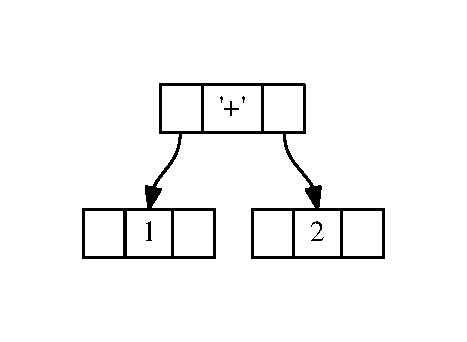
\includegraphics[width=\textwidth,height=\textheight/2,keepaspectratio=true]{dot_inline_dotgraph_2}}
\end{DoxyImageNoCaption}
\end{center}


Example\+: expression is $(1 + 2) + 3$

\begin{center}

\begin{DoxyImageNoCaption}
  \mbox{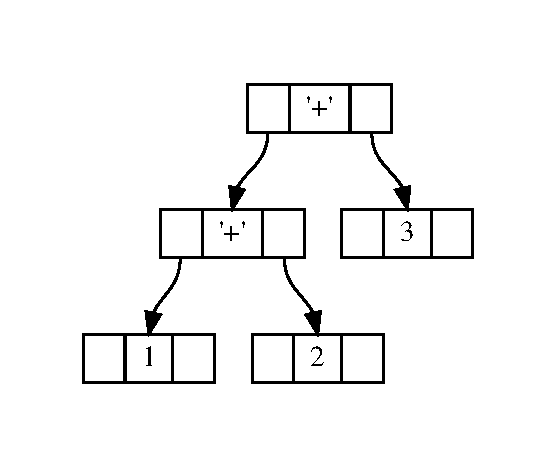
\includegraphics[width=\textwidth,height=\textheight/2,keepaspectratio=true]{dot_inline_dotgraph_3}}
\end{DoxyImageNoCaption}
\end{center}
\hypertarget{index_development}{}\section{Development}\label{index_development}
\hypertarget{index_quick_links}{}\subsection{Quick Links}\label{index_quick_links}

\begin{DoxyItemize}
\item Main library interface file for \hyperlink{expression_8h}{expression.\+h}
\item Main library implementation file for \hyperlink{expression_8c}{expression.\+c}
\end{DoxyItemize}\hypertarget{index_debug_info}{}\subsection{Helpful for Debugging}\label{index_debug_info}

\begin{DoxyItemize}
\item valgrind --tool=memcheck --track-\/origins=yes --undef-\/value-\/errors=yes --leak-\/check=full ./expr \char`\"{}1 + 2\char`\"{}
\item valgrind --tool=memcheck --track-\/origins=yes --undef-\/value-\/errors=yes --leak-\/check=full ./expr \char`\"{}1 + 2\char`\"{}
\item target remote $\vert$ /usr/lib/valgrind/../../bin/vgdb
\end{DoxyItemize}\hypertarget{index_future_changes}{}\subsection{Future Wish List}\label{index_future_changes}

\begin{DoxyItemize}
\item Make string\+\_\+to\+\_\+expression take a start index parameter. This would allow recursive calls to not need temporary string buffers and syntax errors to contain proper index numbers.
\item Handle floats and doubles
\item Handle builtin functions 
\end{DoxyItemize}
\chapter{C Expressions}
\label{md_README}
\Hypertarget{md_README}
This is a mathematical expressions library for C.

\section*{Features}


\begin{DoxyItemize}
\item Symbolic variables
\item Workspaces
\end{DoxyItemize}

Checkout the \href{https://linux4life798.github.io/expressions/html}{\tt Doxygen documentation}. 
\chapter{Test List}
\label{test}
\Hypertarget{test}

\begin{DoxyRefList}
\item[\label{test__test000001}%
\hypertarget{test__test000001}{}%
Global \hyperlink{expression__lite_8h_a63988c00ace0261c4896f132f5f86fda}{string\+\_\+to\+\_\+expression} (size\+\_\+t str\+\_\+len, char const $\ast$str)]Test for negative values 
\end{DoxyRefList}
\chapter{Todo List}
\label{todo}
\Hypertarget{todo}

\begin{DoxyRefList}
\item[\label{todo__todo000001}%
\Hypertarget{todo__todo000001}%
Global \hyperlink{expression__lite_8h_a63988c00ace0261c4896f132f5f86fda}{string\+\_\+to\+\_\+expression} (size\+\_\+t str\+\_\+len, char const $\ast$str)]Allow symbols to be detected when they start with numeric digits also. \hyperlink{symbolic_8h_a78aa047f421c2d8ab5fab3c72d123d1b}{string\+\_\+to\+\_\+sym} is already compatible. 

Do series of additional syntax checks here. 

Syntax Check\+: Check that level==0 

Syntax Check\+: Check that oparen\+\_\+count==cparen\+\_\+count  
\item[\label{todo__todo000005}%
\Hypertarget{todo__todo000005}%
Global \hyperlink{symbolic_8h_a51d47153d7323b2941308b506bd90578}{sym\+\_\+new\+\_\+name} (char $\ast$name)]Should probably check that the name contains valid chars (printable)  
\item[\label{todo__todo000006}%
\Hypertarget{todo__todo000006}%
Global \hyperlink{workspace_8h_a3af2e8d4387ce8986db09a9eb7328bc1}{workspace\+\_\+get} (char $\ast$name)]Create a return value for bad name like \hyperlink{workspace_8h_a536b0f47bc3b9177d1aaca025a05515a}{workspace\+\_\+set} with W\+O\+R\+K\+S\+P\+A\+C\+E\+\_\+\+N\+A\+ME 
\end{DoxyRefList}
\chapter{Bug List}
\label{bug}
\Hypertarget{bug}

\begin{DoxyRefList}
\item[\label{bug__bug000001}%
\hypertarget{bug__bug000001}{}%
Global \hyperlink{expression__lite_8h_a63988c00ace0261c4896f132f5f86fda}{string\+\_\+to\+\_\+expression} (size\+\_\+t str\+\_\+len, char const $\ast$str)]Cannot parse negative numbers \begin{DoxyWarning}{Warning}
Symbols must start with A\+L\+P\+H\+A chars to be properly identified.
\end{DoxyWarning}

\end{DoxyRefList}
\chapter{Data Structure Index}
\section{Data Structures}
Here are the data structures with brief descriptions\+:\begin{DoxyCompactList}
\item\contentsline{section}{\hyperlink{structexpression}{expression} \\*The stored representation of mathematical expressions }{\pageref{structexpression}}{}
\item\contentsline{section}{\hyperlink{unionexpression__data}{expression\+\_\+data} \\*Expression data container }{\pageref{unionexpression__data}}{}
\item\contentsline{section}{\hyperlink{structexpression__data__tree}{expression\+\_\+data\+\_\+tree} \\*Expression data container for the expanded expression }{\pageref{structexpression__data__tree}}{}
\item\contentsline{section}{\hyperlink{structsym}{sym} \\*A named symbol type }{\pageref{structsym}}{}
\item\contentsline{section}{\hyperlink{structvalue}{value} \\*Represents a numeric value or an error }{\pageref{structvalue}}{}
\item\contentsline{section}{\hyperlink{unionvalue__data}{value\+\_\+data} \\*Value data container provider }{\pageref{unionvalue__data}}{}
\end{DoxyCompactList}

\chapter{File Index}
\section{File List}
Here is a list of all files with brief descriptions\+:\begin{DoxyCompactList}
\item\contentsline{section}{\hyperlink{errors_8c}{errors.\+c} }{\pageref{errors_8c}}{}
\item\contentsline{section}{\hyperlink{errors_8h}{errors.\+h} }{\pageref{errors_8h}}{}
\item\contentsline{section}{\hyperlink{expression_8c}{expression.\+c} \\*A compact math expression engine }{\pageref{expression_8c}}{}
\item\contentsline{section}{\hyperlink{expression_8h}{expression.\+h} \\*A compact math expression engine }{\pageref{expression_8h}}{}
\item\contentsline{section}{\hyperlink{expression__lite_8h}{expression\+\_\+lite.\+h} }{\pageref{expression__lite_8h}}{}
\item\contentsline{section}{\hyperlink{main_8c}{main.\+c} }{\pageref{main_8c}}{}
\item\contentsline{section}{\hyperlink{symbolic_8c}{symbolic.\+c} }{\pageref{symbolic_8c}}{}
\item\contentsline{section}{\hyperlink{symbolic_8h}{symbolic.\+h} }{\pageref{symbolic_8h}}{}
\item\contentsline{section}{\hyperlink{types_8c}{types.\+c} }{\pageref{types_8c}}{}
\item\contentsline{section}{\hyperlink{types_8h}{types.\+h} }{\pageref{types_8h}}{}
\item\contentsline{section}{\hyperlink{workspace_8c}{workspace.\+c} }{\pageref{workspace_8c}}{}
\item\contentsline{section}{\hyperlink{workspace_8h}{workspace.\+h} }{\pageref{workspace_8h}}{}
\end{DoxyCompactList}

\chapter{Data Structure Documentation}
\hypertarget{structexpression}{\section{expression Struct Reference}
\label{structexpression}\index{expression@{expression}}
}


The stored representation of mathematical expressions.  




{\ttfamily \#include $<$expression.\+h$>$}



Collaboration diagram for expression\+:\nopagebreak
\begin{figure}[H]
\begin{center}
\leavevmode
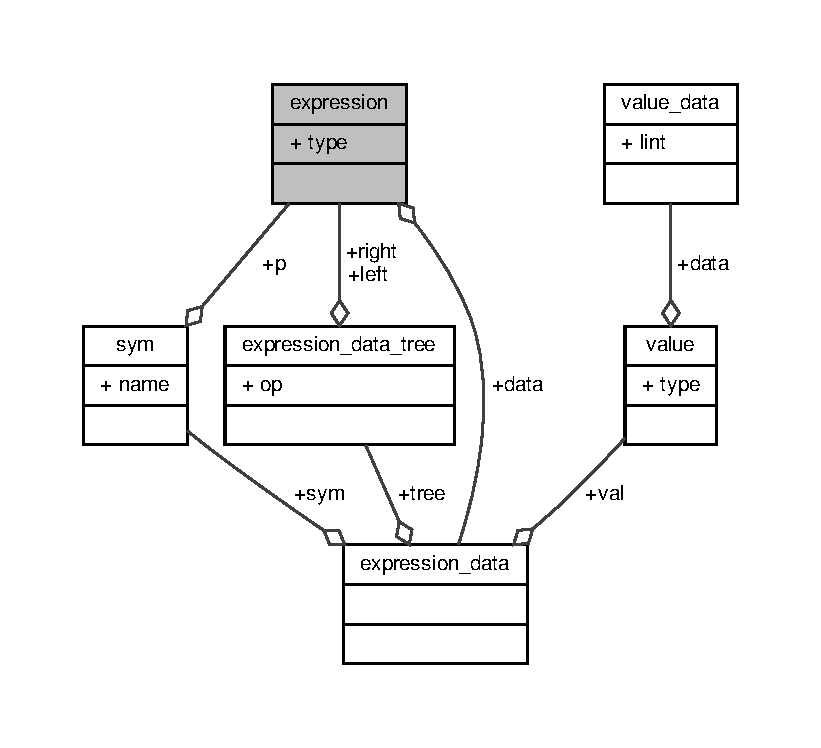
\includegraphics[width=350pt]{structexpression__coll__graph}
\end{center}
\end{figure}
\subsection*{Data Fields}
\begin{DoxyCompactItemize}
\item 
enum \hyperlink{expression_8h_a5a6601c4e142145f0e87051cb21ece0f}{expression\+\_\+type} \hyperlink{structexpression_a6c50b44c70231c1b3752f8516daa967c}{type}
\begin{DoxyCompactList}\small\item\em The expression's selected type. \end{DoxyCompactList}\item 
union \hyperlink{unionexpression__data}{expression\+\_\+data} \hyperlink{structexpression_addb4bda6d311d21f3fd2bfdd12fc70ab}{data}
\begin{DoxyCompactList}\small\item\em The expression's data corresponding to it's \hyperlink{structexpression_a6c50b44c70231c1b3752f8516daa967c}{type}. \end{DoxyCompactList}\end{DoxyCompactItemize}


\subsection{Detailed Description}
The stored representation of mathematical expressions. 

An expression is either an expanded value of an operation on two other sub-\/expressions, a direct value (evaluated expression), or a symbolic expression. An expression consists of an \hyperlink{expression_8h_a5a6601c4e142145f0e87051cb21ece0f}{expression\+\_\+type} and it's \hyperlink{unionexpression__data}{expression\+\_\+data}.\begin{DoxyNote}{Note}
New types must have an entry in the \hyperlink{structexpression_a6c50b44c70231c1b3752f8516daa967c}{type} enumeration and an associated entry in the \hyperlink{structexpression_addb4bda6d311d21f3fd2bfdd12fc70ab}{data} union. 
\end{DoxyNote}


\subsection{Field Documentation}
\hypertarget{structexpression_addb4bda6d311d21f3fd2bfdd12fc70ab}{\index{expression@{expression}!data@{data}}
\index{data@{data}!expression@{expression}}
\subsubsection[{data}]{\setlength{\rightskip}{0pt plus 5cm}union {\bf expression\+\_\+data} data}}\label{structexpression_addb4bda6d311d21f3fd2bfdd12fc70ab}


The expression's data corresponding to it's \hyperlink{structexpression_a6c50b44c70231c1b3752f8516daa967c}{type}. 

\hypertarget{structexpression_a6c50b44c70231c1b3752f8516daa967c}{\index{expression@{expression}!type@{type}}
\index{type@{type}!expression@{expression}}
\subsubsection[{type}]{\setlength{\rightskip}{0pt plus 5cm}enum {\bf expression\+\_\+type} type}}\label{structexpression_a6c50b44c70231c1b3752f8516daa967c}


The expression's selected type. 



The documentation for this struct was generated from the following file\+:\begin{DoxyCompactItemize}
\item 
\hyperlink{expression_8h}{expression.\+h}\end{DoxyCompactItemize}

\hypertarget{unionexpression__data}{\section{expression\+\_\+data Union Reference}
\label{unionexpression__data}\index{expression\+\_\+data@{expression\+\_\+data}}
}


Expression data container.  




{\ttfamily \#include $<$expression.\+h$>$}



Collaboration diagram for expression\+\_\+data\+:\nopagebreak
\begin{figure}[H]
\begin{center}
\leavevmode
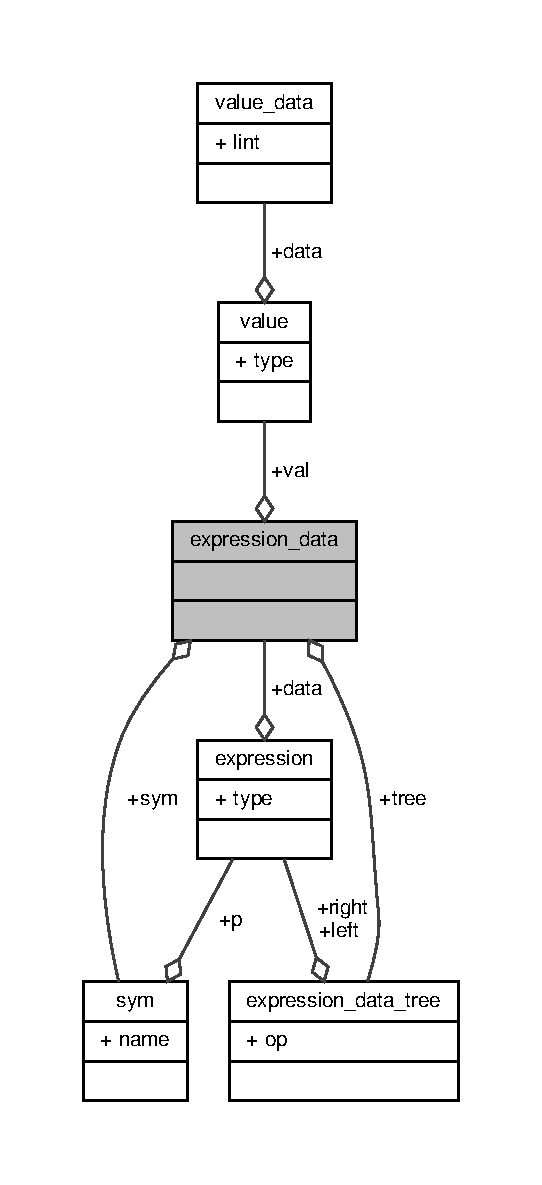
\includegraphics[height=550pt]{unionexpression__data__coll__graph}
\end{center}
\end{figure}
\subsection*{Data Fields}
\begin{DoxyCompactItemize}
\item 
\hyperlink{types_8h_ae4d4f561b975159d5852cb2c30bf20ef}{value\+\_\+t} \hyperlink{unionexpression__data_a9999269c3069b319f17690c708789d42}{val}
\begin{DoxyCompactList}\small\item\em Value for E\+X\+P\+\_\+\+V\+A\+L\+U\+E type. \end{DoxyCompactList}\item 
struct \hyperlink{structexpression__data__tree}{expression\+\_\+data\+\_\+tree} \hyperlink{unionexpression__data_a786f772ef255a1ea6fbb97622b000bc1}{tree}
\begin{DoxyCompactList}\small\item\em Data for E\+X\+P\+\_\+\+T\+R\+E\+E type. \end{DoxyCompactList}\item 
\hyperlink{symbolic_8h_a32ce0f63fa539078e25332dae6b7c77c}{sym\+\_\+t} \hyperlink{unionexpression__data_a09af8ed794d8611cb68c5b68283c260f}{sym}
\begin{DoxyCompactList}\small\item\em Data for E\+X\+P\+\_\+\+S\+Y\+M\+B\+O\+L\+I\+C type. \end{DoxyCompactList}\end{DoxyCompactItemize}


\subsection{Detailed Description}
Expression data container. 

This union allows for the use of all the different expression data containers that corresponding to each \hyperlink{expression_8h_a5a6601c4e142145f0e87051cb21ece0f}{expression\+\_\+type}. 

\subsection{Field Documentation}
\hypertarget{unionexpression__data_a09af8ed794d8611cb68c5b68283c260f}{\index{expression\+\_\+data@{expression\+\_\+data}!sym@{sym}}
\index{sym@{sym}!expression\+\_\+data@{expression\+\_\+data}}
\subsubsection[{sym}]{\setlength{\rightskip}{0pt plus 5cm}{\bf sym\+\_\+t} {\bf sym}}}\label{unionexpression__data_a09af8ed794d8611cb68c5b68283c260f}


Data for E\+X\+P\+\_\+\+S\+Y\+M\+B\+O\+L\+I\+C type. 

\hypertarget{unionexpression__data_a786f772ef255a1ea6fbb97622b000bc1}{\index{expression\+\_\+data@{expression\+\_\+data}!tree@{tree}}
\index{tree@{tree}!expression\+\_\+data@{expression\+\_\+data}}
\subsubsection[{tree}]{\setlength{\rightskip}{0pt plus 5cm}struct {\bf expression\+\_\+data\+\_\+tree} tree}}\label{unionexpression__data_a786f772ef255a1ea6fbb97622b000bc1}


Data for E\+X\+P\+\_\+\+T\+R\+E\+E type. 

\hypertarget{unionexpression__data_a9999269c3069b319f17690c708789d42}{\index{expression\+\_\+data@{expression\+\_\+data}!val@{val}}
\index{val@{val}!expression\+\_\+data@{expression\+\_\+data}}
\subsubsection[{val}]{\setlength{\rightskip}{0pt plus 5cm}{\bf value\+\_\+t} val}}\label{unionexpression__data_a9999269c3069b319f17690c708789d42}


Value for E\+X\+P\+\_\+\+V\+A\+L\+U\+E type. 



The documentation for this union was generated from the following file\+:\begin{DoxyCompactItemize}
\item 
\hyperlink{expression_8h}{expression.\+h}\end{DoxyCompactItemize}

\hypertarget{structexpression__data__tree}{\section{expression\+\_\+data\+\_\+tree Struct Reference}
\label{structexpression__data__tree}\index{expression\+\_\+data\+\_\+tree@{expression\+\_\+data\+\_\+tree}}
}


Expression data container for the expanded expression.  




{\ttfamily \#include $<$expression.\+h$>$}



Collaboration diagram for expression\+\_\+data\+\_\+tree\+:\nopagebreak
\begin{figure}[H]
\begin{center}
\leavevmode
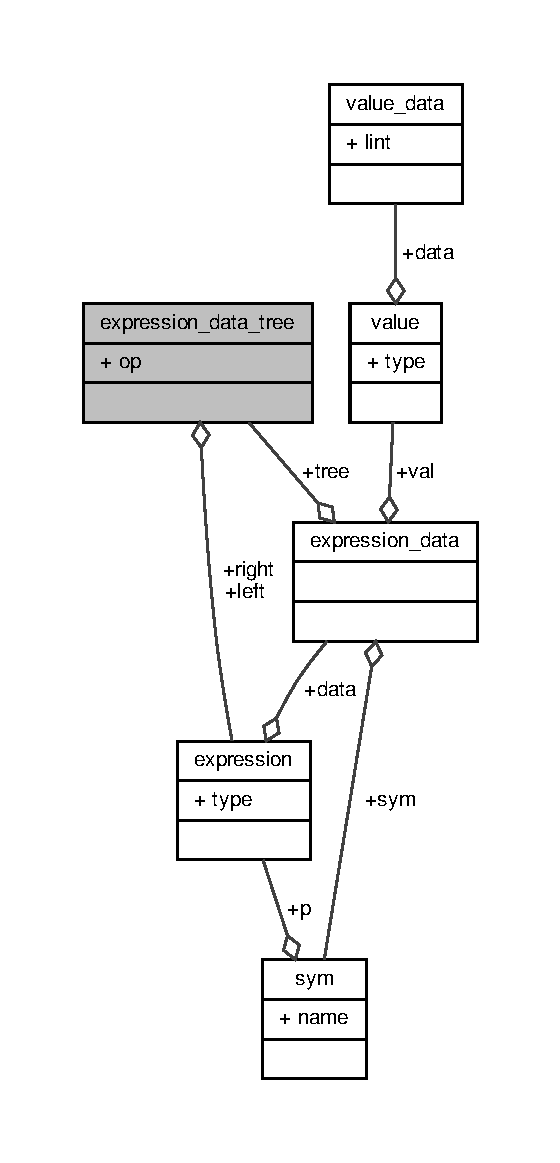
\includegraphics[height=550pt]{structexpression__data__tree__coll__graph}
\end{center}
\end{figure}
\subsection*{Data Fields}
\begin{DoxyCompactItemize}
\item 
char \hyperlink{structexpression__data__tree_a3d5c605540ca9e9431799d5a79cb94b0}{op}
\begin{DoxyCompactList}\small\item\em The joining operation of the two two sub expressions. \end{DoxyCompactList}\item 
\hyperlink{expression__lite_8h_ac198bce62637e5d742da0218d544a7ac}{expression\+\_\+t} \hyperlink{structexpression__data__tree_a46f4a906ae330c3598e899fc77c3d17a}{left}
\begin{DoxyCompactList}\small\item\em Left sub-\/expression. \end{DoxyCompactList}\item 
\hyperlink{expression__lite_8h_ac198bce62637e5d742da0218d544a7ac}{expression\+\_\+t} \hyperlink{structexpression__data__tree_ad77c9db9f894879970e67e6cb081db60}{right}
\begin{DoxyCompactList}\small\item\em Right sub-\/expression. \end{DoxyCompactList}\end{DoxyCompactItemize}


\subsection{Detailed Description}
Expression data container for the expanded expression. 

Expanded tree expressions are composed of an operation that joins a left sub-\/expression and a right rub-\/expression. 

\subsection{Field Documentation}
\hypertarget{structexpression__data__tree_a46f4a906ae330c3598e899fc77c3d17a}{\index{expression\+\_\+data\+\_\+tree@{expression\+\_\+data\+\_\+tree}!left@{left}}
\index{left@{left}!expression\+\_\+data\+\_\+tree@{expression\+\_\+data\+\_\+tree}}
\subsubsection[{left}]{\setlength{\rightskip}{0pt plus 5cm}{\bf expression\+\_\+t} left}}\label{structexpression__data__tree_a46f4a906ae330c3598e899fc77c3d17a}


Left sub-\/expression. 

\hypertarget{structexpression__data__tree_a3d5c605540ca9e9431799d5a79cb94b0}{\index{expression\+\_\+data\+\_\+tree@{expression\+\_\+data\+\_\+tree}!op@{op}}
\index{op@{op}!expression\+\_\+data\+\_\+tree@{expression\+\_\+data\+\_\+tree}}
\subsubsection[{op}]{\setlength{\rightskip}{0pt plus 5cm}char op}}\label{structexpression__data__tree_a3d5c605540ca9e9431799d5a79cb94b0}


The joining operation of the two two sub expressions. 

\begin{DoxyNote}{Note}
Previously implemented using enumerations, but proved to be more of a burden. 
\end{DoxyNote}
\hypertarget{structexpression__data__tree_ad77c9db9f894879970e67e6cb081db60}{\index{expression\+\_\+data\+\_\+tree@{expression\+\_\+data\+\_\+tree}!right@{right}}
\index{right@{right}!expression\+\_\+data\+\_\+tree@{expression\+\_\+data\+\_\+tree}}
\subsubsection[{right}]{\setlength{\rightskip}{0pt plus 5cm}{\bf expression\+\_\+t} right}}\label{structexpression__data__tree_ad77c9db9f894879970e67e6cb081db60}


Right sub-\/expression. 



The documentation for this struct was generated from the following file\+:\begin{DoxyCompactItemize}
\item 
\hyperlink{expression_8h}{expression.\+h}\end{DoxyCompactItemize}

\hypertarget{structsym}{\section{sym Struct Reference}
\label{structsym}\index{sym@{sym}}
}


A named symbol type.  




{\ttfamily \#include $<$symbolic.\+h$>$}



Collaboration diagram for sym\+:\nopagebreak
\begin{figure}[H]
\begin{center}
\leavevmode
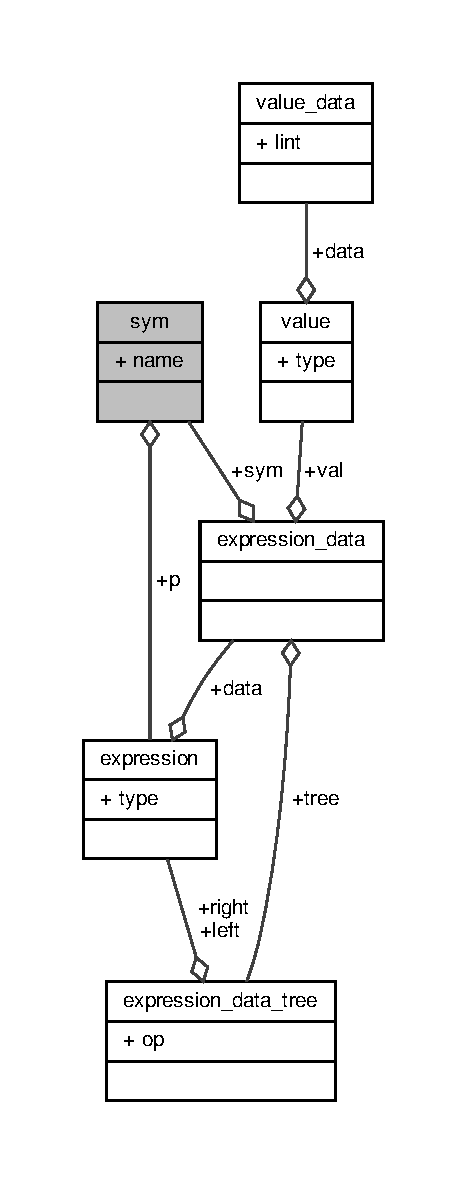
\includegraphics[height=550pt]{structsym__coll__graph}
\end{center}
\end{figure}
\subsection*{Data Fields}
\begin{DoxyCompactItemize}
\item 
char \hyperlink{structsym_ab3675903eb67a0a887759b93892151a5}{name} \mbox{[}\hyperlink{symbolic_8h_aeb7545cf4c9c6df72954b9409a00a885}{S\+Y\+M\+B\+O\+L\+I\+C\+\_\+\+N\+A\+M\+E\+\_\+\+S\+I\+Z\+E}\mbox{]}
\begin{DoxyCompactList}\small\item\em The symbol name. \end{DoxyCompactList}\item 
struct \hyperlink{structexpression}{expression} $\ast$ \hyperlink{structsym_a0796b3f7efa6a72c76822710e20c6060}{p}
\begin{DoxyCompactList}\small\item\em The symbol parameter. \end{DoxyCompactList}\end{DoxyCompactItemize}


\subsection{Detailed Description}
A named symbol type. 

A symbol can refer to a variable or function. The field p is N\+U\+L\+L when no parameter exists. 

\subsection{Field Documentation}
\hypertarget{structsym_ab3675903eb67a0a887759b93892151a5}{\index{sym@{sym}!name@{name}}
\index{name@{name}!sym@{sym}}
\subsubsection[{name}]{\setlength{\rightskip}{0pt plus 5cm}char name\mbox{[}{\bf S\+Y\+M\+B\+O\+L\+I\+C\+\_\+\+N\+A\+M\+E\+\_\+\+S\+I\+Z\+E}\mbox{]}}}\label{structsym_ab3675903eb67a0a887759b93892151a5}


The symbol name. 

\hypertarget{structsym_a0796b3f7efa6a72c76822710e20c6060}{\index{sym@{sym}!p@{p}}
\index{p@{p}!sym@{sym}}
\subsubsection[{p}]{\setlength{\rightskip}{0pt plus 5cm}struct {\bf expression}$\ast$ p}}\label{structsym_a0796b3f7efa6a72c76822710e20c6060}


The symbol parameter. 



The documentation for this struct was generated from the following file\+:\begin{DoxyCompactItemize}
\item 
\hyperlink{symbolic_8h}{symbolic.\+h}\end{DoxyCompactItemize}

\hypertarget{structvalue}{}\section{value Struct Reference}
\label{structvalue}\index{value@{value}}


Represents a numeric value or an error.  




{\ttfamily \#include $<$types.\+h$>$}



Collaboration diagram for value\+:
\nopagebreak
\begin{figure}[H]
\begin{center}
\leavevmode
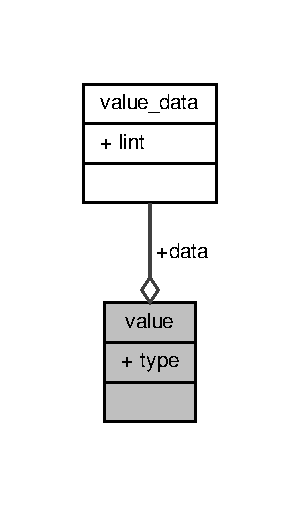
\includegraphics[width=144pt]{structvalue__coll__graph}
\end{center}
\end{figure}
\subsection*{Data Fields}
\begin{DoxyCompactItemize}
\item 
enum \hyperlink{types_8h_a2763ddd86ab6e5f5f4c34c0561d4cd39}{value\+\_\+types} \hyperlink{structvalue_a51293d8a9946f28f389010bf83820015}{type}
\item 
union \hyperlink{unionvalue__data}{value\+\_\+data} \hyperlink{structvalue_a7a505de18bdf859cc9246069c70c18b5}{data}
\end{DoxyCompactItemize}


\subsection{Detailed Description}
Represents a numeric value or an error. 

This is the structure that abstractly represents numeric values including undefined values and errors they may be associated with. 

\subsection{Field Documentation}
\mbox{\Hypertarget{structvalue_a7a505de18bdf859cc9246069c70c18b5}\label{structvalue_a7a505de18bdf859cc9246069c70c18b5}} 
\index{value@{value}!data@{data}}
\index{data@{data}!value@{value}}
\subsubsection{\texorpdfstring{data}{data}}
{\footnotesize\ttfamily union \hyperlink{unionvalue__data}{value\+\_\+data} data}

\mbox{\Hypertarget{structvalue_a51293d8a9946f28f389010bf83820015}\label{structvalue_a51293d8a9946f28f389010bf83820015}} 
\index{value@{value}!type@{type}}
\index{type@{type}!value@{value}}
\subsubsection{\texorpdfstring{type}{type}}
{\footnotesize\ttfamily enum \hyperlink{types_8h_a2763ddd86ab6e5f5f4c34c0561d4cd39}{value\+\_\+types} type}



The documentation for this struct was generated from the following file\+:\begin{DoxyCompactItemize}
\item 
\hyperlink{types_8h}{types.\+h}\end{DoxyCompactItemize}

\hypertarget{unionvalue__data}{\section{value\+\_\+data Union Reference}
\label{unionvalue__data}\index{value\+\_\+data@{value\+\_\+data}}
}


value data container provider  




{\ttfamily \#include $<$types.\+h$>$}



Collaboration diagram for value\+\_\+data\+:\nopagebreak
\begin{figure}[H]
\begin{center}
\leavevmode
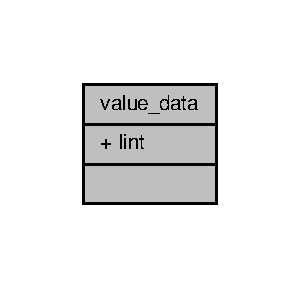
\includegraphics[width=144pt]{unionvalue__data__coll__graph}
\end{center}
\end{figure}
\subsection*{Data Fields}
\begin{DoxyCompactItemize}
\item 
\hyperlink{types_8h_a5b2030ae244cd6621f11f4bf6d181dbf}{sys\+\_\+int\+\_\+long} \hyperlink{unionvalue__data_a16d792f39cc926e4b92c279ab3aa68eb}{lint}
\end{DoxyCompactItemize}


\subsection{Detailed Description}
value data container provider 

\subsection{Field Documentation}
\hypertarget{unionvalue__data_a16d792f39cc926e4b92c279ab3aa68eb}{\index{value\+\_\+data@{value\+\_\+data}!lint@{lint}}
\index{lint@{lint}!value\+\_\+data@{value\+\_\+data}}
\subsubsection[{lint}]{\setlength{\rightskip}{0pt plus 5cm}{\bf sys\+\_\+int\+\_\+long} lint}}\label{unionvalue__data_a16d792f39cc926e4b92c279ab3aa68eb}


The documentation for this union was generated from the following file\+:\begin{DoxyCompactItemize}
\item 
\hyperlink{types_8h}{types.\+h}\end{DoxyCompactItemize}

\chapter{File Documentation}
\hypertarget{doc_8dox}{\section{doc.\+dox File Reference}
\label{doc_8dox}\index{doc.\+dox@{doc.\+dox}}
}

\hypertarget{errors_8c}{\section{errors.\+c File Reference}
\label{errors_8c}\index{errors.\+c@{errors.\+c}}
}
{\ttfamily \#include $<$stdio.\+h$>$}\\*
{\ttfamily \#include $<$stdlib.\+h$>$}\\*
{\ttfamily \#include $<$stdarg.\+h$>$}\\*
{\ttfamily \#include $<$assert.\+h$>$}\\*
{\ttfamily \#include \char`\"{}errors.\+h\char`\"{}}\\*
Include dependency graph for errors.\+c\+:\nopagebreak
\begin{figure}[H]
\begin{center}
\leavevmode
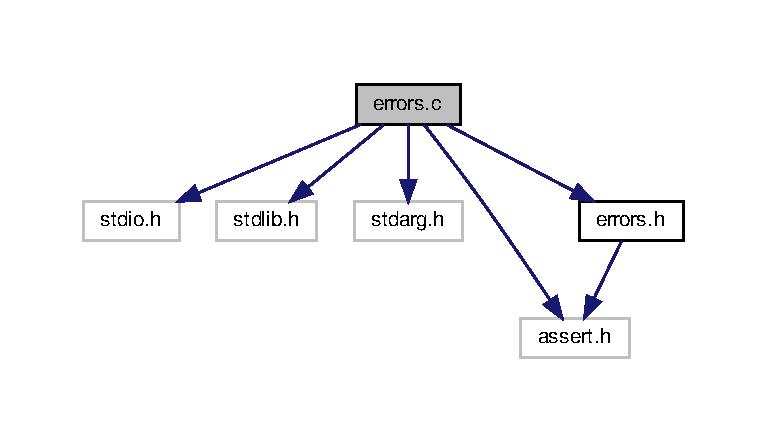
\includegraphics[width=350pt]{errors_8c__incl}
\end{center}
\end{figure}
\subsection*{Functions}
\begin{DoxyCompactItemize}
\item 
void \hyperlink{errors_8c_acffe5034f6694d4d88d78a2b4eb87c06}{rerror} (char const $\ast$fmt,...)
\item 
void \hyperlink{errors_8c_a4586b9204c37a7050d838ccfcbde3e3d}{pferror} (const char $\ast$function\+\_\+name, char const $\ast$fmt,...)
\end{DoxyCompactItemize}


\subsection{Function Documentation}
\hypertarget{errors_8c_a4586b9204c37a7050d838ccfcbde3e3d}{\index{errors.\+c@{errors.\+c}!pferror@{pferror}}
\index{pferror@{pferror}!errors.\+c@{errors.\+c}}
\subsubsection[{pferror}]{\setlength{\rightskip}{0pt plus 5cm}void pferror (
\begin{DoxyParamCaption}
\item[{const char $\ast$}]{function\+\_\+name, }
\item[{char const $\ast$}]{fmt, }
\item[{}]{...}
\end{DoxyParamCaption}
)}}\label{errors_8c_a4586b9204c37a7050d838ccfcbde3e3d}
\hypertarget{errors_8c_acffe5034f6694d4d88d78a2b4eb87c06}{\index{errors.\+c@{errors.\+c}!rerror@{rerror}}
\index{rerror@{rerror}!errors.\+c@{errors.\+c}}
\subsubsection[{rerror}]{\setlength{\rightskip}{0pt plus 5cm}void rerror (
\begin{DoxyParamCaption}
\item[{char const $\ast$}]{fmt, }
\item[{}]{...}
\end{DoxyParamCaption}
)}}\label{errors_8c_acffe5034f6694d4d88d78a2b4eb87c06}

\hypertarget{errors_8h}{\section{errors.\+h File Reference}
\label{errors_8h}\index{errors.\+h@{errors.\+h}}
}
{\ttfamily \#include $<$assert.\+h$>$}\\*
Include dependency graph for errors.\+h\+:\nopagebreak
\begin{figure}[H]
\begin{center}
\leavevmode
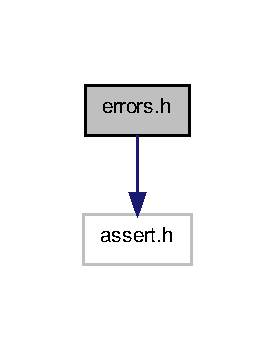
\includegraphics[width=132pt]{errors_8h__incl}
\end{center}
\end{figure}
\subsection*{Functions}
\begin{DoxyCompactItemize}
\item 
void \hyperlink{errors_8h_acffe5034f6694d4d88d78a2b4eb87c06}{rerror} (char const $\ast$fmt,...)
\item 
void \hyperlink{errors_8h_a4586b9204c37a7050d838ccfcbde3e3d}{pferror} (const char $\ast$function\+\_\+name, char const $\ast$fmt,...)
\end{DoxyCompactItemize}


\subsection{Function Documentation}
\hypertarget{errors_8h_a4586b9204c37a7050d838ccfcbde3e3d}{\index{errors.\+h@{errors.\+h}!pferror@{pferror}}
\index{pferror@{pferror}!errors.\+h@{errors.\+h}}
\subsubsection[{pferror}]{\setlength{\rightskip}{0pt plus 5cm}void pferror (
\begin{DoxyParamCaption}
\item[{const char $\ast$}]{function\+\_\+name, }
\item[{char const $\ast$}]{fmt, }
\item[{}]{...}
\end{DoxyParamCaption}
)}}\label{errors_8h_a4586b9204c37a7050d838ccfcbde3e3d}
\hypertarget{errors_8h_acffe5034f6694d4d88d78a2b4eb87c06}{\index{errors.\+h@{errors.\+h}!rerror@{rerror}}
\index{rerror@{rerror}!errors.\+h@{errors.\+h}}
\subsubsection[{rerror}]{\setlength{\rightskip}{0pt plus 5cm}void rerror (
\begin{DoxyParamCaption}
\item[{char const $\ast$}]{fmt, }
\item[{}]{...}
\end{DoxyParamCaption}
)}}\label{errors_8h_acffe5034f6694d4d88d78a2b4eb87c06}

\hypertarget{expression_8c}{}\section{expression.\+c File Reference}
\label{expression_8c}\index{expression.\+c@{expression.\+c}}


A compact math expression engine.  


{\ttfamily \#include $<$stdio.\+h$>$}\newline
{\ttfamily \#include $<$stdlib.\+h$>$}\newline
{\ttfamily \#include $<$string.\+h$>$}\newline
{\ttfamily \#include \char`\"{}types.\+h\char`\"{}}\newline
{\ttfamily \#include \char`\"{}errors.\+h\char`\"{}}\newline
{\ttfamily \#include \char`\"{}symbolic.\+h\char`\"{}}\newline
{\ttfamily \#include \char`\"{}expression.\+h\char`\"{}}\newline
Include dependency graph for expression.\+c\+:
\nopagebreak
\begin{figure}[H]
\begin{center}
\leavevmode
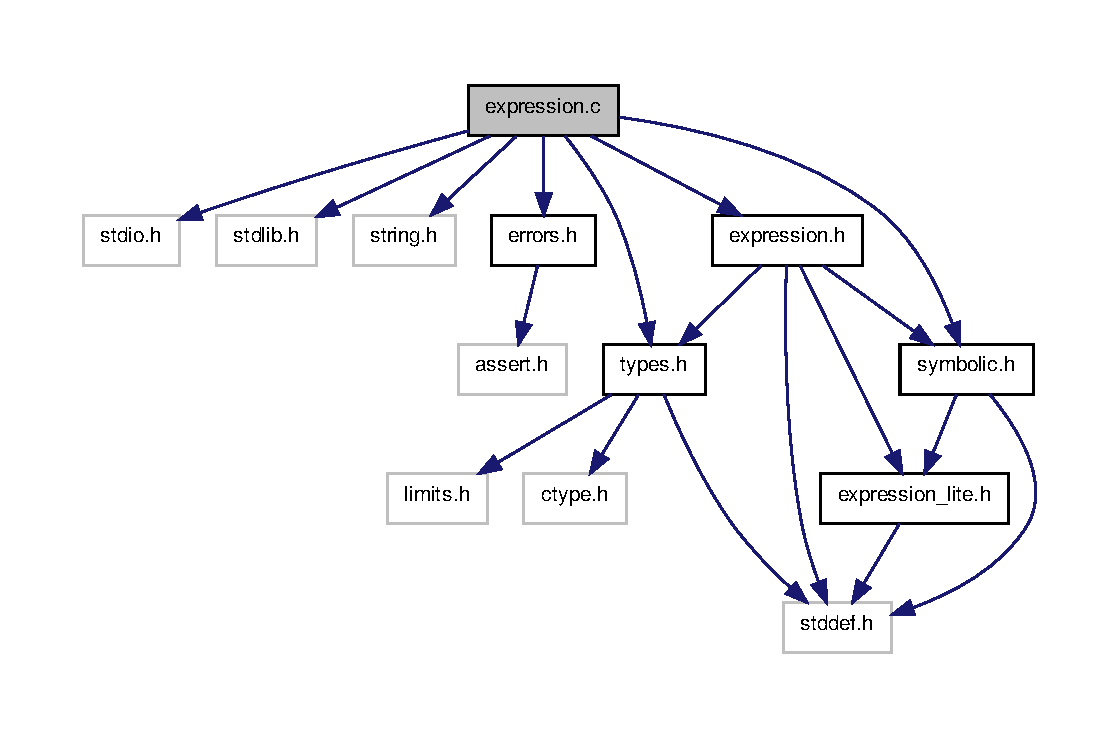
\includegraphics[width=350pt]{expression_8c__incl}
\end{center}
\end{figure}
\subsection*{Functions}
\begin{DoxyCompactItemize}
\item 
\hyperlink{expression__lite_8h_ac198bce62637e5d742da0218d544a7ac}{expression\+\_\+t} \hyperlink{expression_8c_a513e1cb7ae9dbcef50307f2c13e00dd9}{expression\+\_\+new} (void)
\begin{DoxyCompactList}\small\item\em New blank expression. \end{DoxyCompactList}\item 
\hyperlink{expression__lite_8h_ac198bce62637e5d742da0218d544a7ac}{expression\+\_\+t} \hyperlink{expression_8c_a7c44bf0c0e78a10270eeec18a89eb340}{expression\+\_\+new\+\_\+value} (\hyperlink{types_8h_ae4d4f561b975159d5852cb2c30bf20ef}{value\+\_\+t} val)
\item 
\hyperlink{expression__lite_8h_ac198bce62637e5d742da0218d544a7ac}{expression\+\_\+t} \hyperlink{expression_8c_affb6adb350cc9126e06af303607ca812}{expression\+\_\+new\+\_\+tree} (char op, \hyperlink{expression__lite_8h_ac198bce62637e5d742da0218d544a7ac}{expression\+\_\+t} left, \hyperlink{expression__lite_8h_ac198bce62637e5d742da0218d544a7ac}{expression\+\_\+t} right)
\item 
\hyperlink{expression__lite_8h_ac198bce62637e5d742da0218d544a7ac}{expression\+\_\+t} \hyperlink{expression_8c_a02b7142f5701d82971d1f21ec20772be}{expression\+\_\+new\+\_\+sym} (\hyperlink{symbolic_8h_a32ce0f63fa539078e25332dae6b7c77c}{sym\+\_\+t} \hyperlink{structsym}{sym})
\item 
void \hyperlink{expression_8c_a6f1cc930ee50ba61adf466fbdf4b1fb2}{expression\+\_\+free} (\hyperlink{expression__lite_8h_ac198bce62637e5d742da0218d544a7ac}{expression\+\_\+t} exp)
\begin{DoxyCompactList}\small\item\em Free an expression. \end{DoxyCompactList}\item 
\hyperlink{types_8h_ae4d4f561b975159d5852cb2c30bf20ef}{value\+\_\+t} \hyperlink{expression_8c_a70f3326a088855f6916f04baf27feed3}{expression\+\_\+evaluate} (\hyperlink{expression__lite_8h_ac198bce62637e5d742da0218d544a7ac}{expression\+\_\+t} exp)
\item 
void \hyperlink{expression_8c_aca3bb6ea526afbf4f238a0877fe3e131}{expression\+\_\+to\+\_\+string} (char $\ast$dst\+\_\+str, \hyperlink{expression__lite_8h_ac198bce62637e5d742da0218d544a7ac}{expression\+\_\+t} src\+\_\+exp)
\begin{DoxyCompactList}\small\item\em Expression to String. \end{DoxyCompactList}\item 
size\+\_\+t \hyperlink{expression_8c_aadcbbaeb4759be2826011415c4fc89c0}{number\+\_\+len} (size\+\_\+t str\+\_\+len, char $\ast$str)
\item 
void \hyperlink{expression_8c_a5b815476fd7c2f8ebb81bfde2b024f48}{str\+\_\+cpy} (char $\ast$dest, const char $\ast$src, size\+\_\+t count)
\begin{DoxyCompactList}\small\item\em Same as strncpy, but throws an error if a null character is reached in src. \end{DoxyCompactList}\item 
\hyperlink{expression__lite_8h_ac198bce62637e5d742da0218d544a7ac}{expression\+\_\+t} \hyperlink{expression_8c_a63988c00ace0261c4896f132f5f86fda}{string\+\_\+to\+\_\+expression} (size\+\_\+t str\+\_\+len, char const $\ast$str)
\begin{DoxyCompactList}\small\item\em Convert String to an Expression. \end{DoxyCompactList}\end{DoxyCompactItemize}


\subsection{Detailed Description}
A compact math expression engine. 

\begin{DoxyDate}{Date}
Apr 6, 2014 
\end{DoxyDate}
\begin{DoxyAuthor}{Author}
Craig Hesling 
\end{DoxyAuthor}


\subsection{Function Documentation}
\mbox{\Hypertarget{expression_8c_a70f3326a088855f6916f04baf27feed3}\label{expression_8c_a70f3326a088855f6916f04baf27feed3}} 
\index{expression.\+c@{expression.\+c}!expression\+\_\+evaluate@{expression\+\_\+evaluate}}
\index{expression\+\_\+evaluate@{expression\+\_\+evaluate}!expression.\+c@{expression.\+c}}
\subsubsection{\texorpdfstring{expression\+\_\+evaluate()}{expression\_evaluate()}}
{\footnotesize\ttfamily \hyperlink{types_8h_ae4d4f561b975159d5852cb2c30bf20ef}{value\+\_\+t} expression\+\_\+evaluate (\begin{DoxyParamCaption}\item[{\hyperlink{expression__lite_8h_ac198bce62637e5d742da0218d544a7ac}{expression\+\_\+t}}]{exp }\end{DoxyParamCaption})}

Here is the call graph for this function\+:
\nopagebreak
\begin{figure}[H]
\begin{center}
\leavevmode
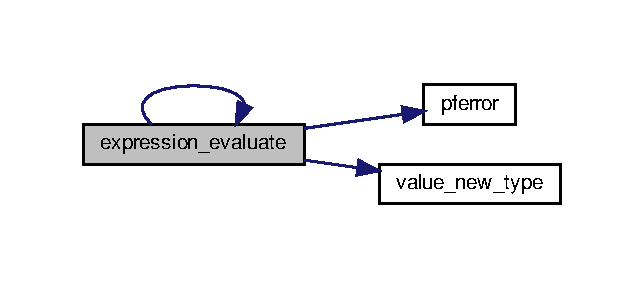
\includegraphics[width=309pt]{expression_8c_a70f3326a088855f6916f04baf27feed3_cgraph}
\end{center}
\end{figure}
\mbox{\Hypertarget{expression_8c_a6f1cc930ee50ba61adf466fbdf4b1fb2}\label{expression_8c_a6f1cc930ee50ba61adf466fbdf4b1fb2}} 
\index{expression.\+c@{expression.\+c}!expression\+\_\+free@{expression\+\_\+free}}
\index{expression\+\_\+free@{expression\+\_\+free}!expression.\+c@{expression.\+c}}
\subsubsection{\texorpdfstring{expression\+\_\+free()}{expression\_free()}}
{\footnotesize\ttfamily void expression\+\_\+free (\begin{DoxyParamCaption}\item[{\hyperlink{expression__lite_8h_ac198bce62637e5d742da0218d544a7ac}{expression\+\_\+t}}]{exp }\end{DoxyParamCaption})}



Free an expression. 


\begin{DoxyParams}{Parameters}
{\em exp} & The expression to free \\
\hline
\end{DoxyParams}
Here is the call graph for this function\+:
\nopagebreak
\begin{figure}[H]
\begin{center}
\leavevmode
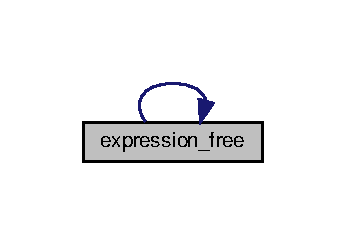
\includegraphics[width=166pt]{expression_8c_a6f1cc930ee50ba61adf466fbdf4b1fb2_cgraph}
\end{center}
\end{figure}
\mbox{\Hypertarget{expression_8c_a513e1cb7ae9dbcef50307f2c13e00dd9}\label{expression_8c_a513e1cb7ae9dbcef50307f2c13e00dd9}} 
\index{expression.\+c@{expression.\+c}!expression\+\_\+new@{expression\+\_\+new}}
\index{expression\+\_\+new@{expression\+\_\+new}!expression.\+c@{expression.\+c}}
\subsubsection{\texorpdfstring{expression\+\_\+new()}{expression\_new()}}
{\footnotesize\ttfamily \hyperlink{expression__lite_8h_ac198bce62637e5d742da0218d544a7ac}{expression\+\_\+t} expression\+\_\+new (\begin{DoxyParamCaption}\item[{void}]{ }\end{DoxyParamCaption})}



New blank expression. 

This function creates the most basic empty expression. \begin{DoxyReturn}{Returns}
A new empty expression 
\end{DoxyReturn}
\mbox{\Hypertarget{expression_8c_a02b7142f5701d82971d1f21ec20772be}\label{expression_8c_a02b7142f5701d82971d1f21ec20772be}} 
\index{expression.\+c@{expression.\+c}!expression\+\_\+new\+\_\+sym@{expression\+\_\+new\+\_\+sym}}
\index{expression\+\_\+new\+\_\+sym@{expression\+\_\+new\+\_\+sym}!expression.\+c@{expression.\+c}}
\subsubsection{\texorpdfstring{expression\+\_\+new\+\_\+sym()}{expression\_new\_sym()}}
{\footnotesize\ttfamily \hyperlink{expression__lite_8h_ac198bce62637e5d742da0218d544a7ac}{expression\+\_\+t} expression\+\_\+new\+\_\+sym (\begin{DoxyParamCaption}\item[{\hyperlink{symbolic_8h_a32ce0f63fa539078e25332dae6b7c77c}{sym\+\_\+t}}]{sym }\end{DoxyParamCaption})}

Here is the call graph for this function\+:
\nopagebreak
\begin{figure}[H]
\begin{center}
\leavevmode
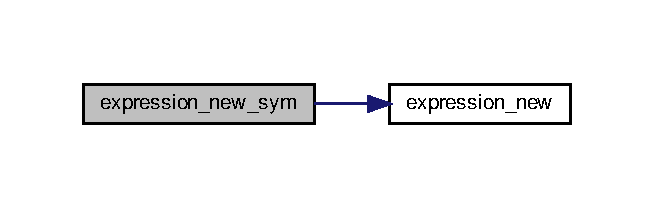
\includegraphics[width=314pt]{expression_8c_a02b7142f5701d82971d1f21ec20772be_cgraph}
\end{center}
\end{figure}
\mbox{\Hypertarget{expression_8c_affb6adb350cc9126e06af303607ca812}\label{expression_8c_affb6adb350cc9126e06af303607ca812}} 
\index{expression.\+c@{expression.\+c}!expression\+\_\+new\+\_\+tree@{expression\+\_\+new\+\_\+tree}}
\index{expression\+\_\+new\+\_\+tree@{expression\+\_\+new\+\_\+tree}!expression.\+c@{expression.\+c}}
\subsubsection{\texorpdfstring{expression\+\_\+new\+\_\+tree()}{expression\_new\_tree()}}
{\footnotesize\ttfamily \hyperlink{expression__lite_8h_ac198bce62637e5d742da0218d544a7ac}{expression\+\_\+t} expression\+\_\+new\+\_\+tree (\begin{DoxyParamCaption}\item[{char}]{op,  }\item[{\hyperlink{expression__lite_8h_ac198bce62637e5d742da0218d544a7ac}{expression\+\_\+t}}]{left,  }\item[{\hyperlink{expression__lite_8h_ac198bce62637e5d742da0218d544a7ac}{expression\+\_\+t}}]{right }\end{DoxyParamCaption})}

Here is the call graph for this function\+:
\nopagebreak
\begin{figure}[H]
\begin{center}
\leavevmode
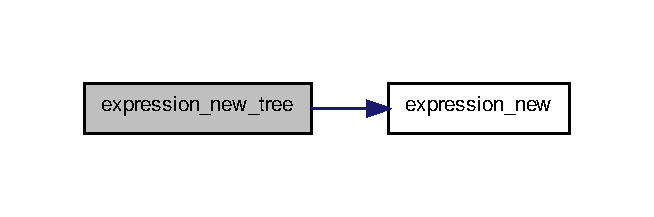
\includegraphics[width=312pt]{expression_8c_affb6adb350cc9126e06af303607ca812_cgraph}
\end{center}
\end{figure}
\mbox{\Hypertarget{expression_8c_a7c44bf0c0e78a10270eeec18a89eb340}\label{expression_8c_a7c44bf0c0e78a10270eeec18a89eb340}} 
\index{expression.\+c@{expression.\+c}!expression\+\_\+new\+\_\+value@{expression\+\_\+new\+\_\+value}}
\index{expression\+\_\+new\+\_\+value@{expression\+\_\+new\+\_\+value}!expression.\+c@{expression.\+c}}
\subsubsection{\texorpdfstring{expression\+\_\+new\+\_\+value()}{expression\_new\_value()}}
{\footnotesize\ttfamily \hyperlink{expression__lite_8h_ac198bce62637e5d742da0218d544a7ac}{expression\+\_\+t} expression\+\_\+new\+\_\+value (\begin{DoxyParamCaption}\item[{\hyperlink{types_8h_ae4d4f561b975159d5852cb2c30bf20ef}{value\+\_\+t}}]{val }\end{DoxyParamCaption})}

Here is the call graph for this function\+:
\nopagebreak
\begin{figure}[H]
\begin{center}
\leavevmode
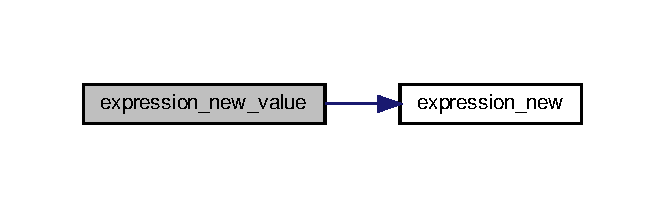
\includegraphics[width=319pt]{expression_8c_a7c44bf0c0e78a10270eeec18a89eb340_cgraph}
\end{center}
\end{figure}
\mbox{\Hypertarget{expression_8c_aca3bb6ea526afbf4f238a0877fe3e131}\label{expression_8c_aca3bb6ea526afbf4f238a0877fe3e131}} 
\index{expression.\+c@{expression.\+c}!expression\+\_\+to\+\_\+string@{expression\+\_\+to\+\_\+string}}
\index{expression\+\_\+to\+\_\+string@{expression\+\_\+to\+\_\+string}!expression.\+c@{expression.\+c}}
\subsubsection{\texorpdfstring{expression\+\_\+to\+\_\+string()}{expression\_to\_string()}}
{\footnotesize\ttfamily void expression\+\_\+to\+\_\+string (\begin{DoxyParamCaption}\item[{char $\ast$}]{dst\+\_\+str,  }\item[{\hyperlink{expression__lite_8h_ac198bce62637e5d742da0218d544a7ac}{expression\+\_\+t}}]{src\+\_\+exp }\end{DoxyParamCaption})}



Expression to String. 

Here is the call graph for this function\+:
\nopagebreak
\begin{figure}[H]
\begin{center}
\leavevmode
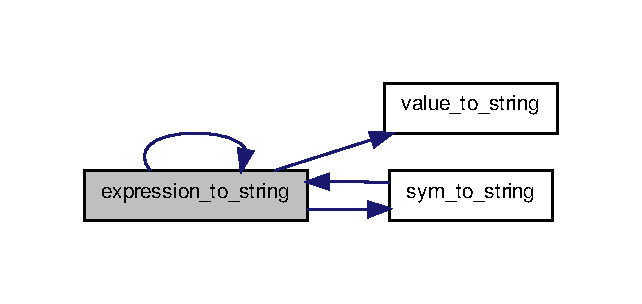
\includegraphics[width=306pt]{expression_8c_aca3bb6ea526afbf4f238a0877fe3e131_cgraph}
\end{center}
\end{figure}
\mbox{\Hypertarget{expression_8c_aadcbbaeb4759be2826011415c4fc89c0}\label{expression_8c_aadcbbaeb4759be2826011415c4fc89c0}} 
\index{expression.\+c@{expression.\+c}!number\+\_\+len@{number\+\_\+len}}
\index{number\+\_\+len@{number\+\_\+len}!expression.\+c@{expression.\+c}}
\subsubsection{\texorpdfstring{number\+\_\+len()}{number\_len()}}
{\footnotesize\ttfamily size\+\_\+t number\+\_\+len (\begin{DoxyParamCaption}\item[{size\+\_\+t}]{str\+\_\+len,  }\item[{char $\ast$}]{str }\end{DoxyParamCaption})}

\mbox{\Hypertarget{expression_8c_a5b815476fd7c2f8ebb81bfde2b024f48}\label{expression_8c_a5b815476fd7c2f8ebb81bfde2b024f48}} 
\index{expression.\+c@{expression.\+c}!str\+\_\+cpy@{str\+\_\+cpy}}
\index{str\+\_\+cpy@{str\+\_\+cpy}!expression.\+c@{expression.\+c}}
\subsubsection{\texorpdfstring{str\+\_\+cpy()}{str\_cpy()}}
{\footnotesize\ttfamily void str\+\_\+cpy (\begin{DoxyParamCaption}\item[{char $\ast$}]{dest,  }\item[{const char $\ast$}]{src,  }\item[{size\+\_\+t}]{count }\end{DoxyParamCaption})}



Same as strncpy, but throws an error if a null character is reached in src. 


\begin{DoxyParams}{Parameters}
{\em dest} & Destination string buffer. \\
\hline
{\em src} & Source string buffer. \\
\hline
{\em count} & The number of bytes to copy. \\
\hline
\end{DoxyParams}
Here is the call graph for this function\+:
\nopagebreak
\begin{figure}[H]
\begin{center}
\leavevmode
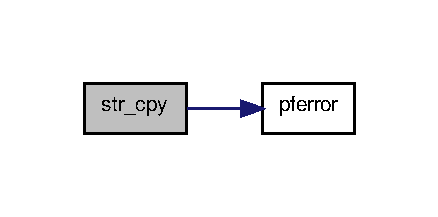
\includegraphics[width=209pt]{expression_8c_a5b815476fd7c2f8ebb81bfde2b024f48_cgraph}
\end{center}
\end{figure}
\mbox{\Hypertarget{expression_8c_a63988c00ace0261c4896f132f5f86fda}\label{expression_8c_a63988c00ace0261c4896f132f5f86fda}} 
\index{expression.\+c@{expression.\+c}!string\+\_\+to\+\_\+expression@{string\+\_\+to\+\_\+expression}}
\index{string\+\_\+to\+\_\+expression@{string\+\_\+to\+\_\+expression}!expression.\+c@{expression.\+c}}
\subsubsection{\texorpdfstring{string\+\_\+to\+\_\+expression()}{string\_to\_expression()}}
{\footnotesize\ttfamily \hyperlink{expression__lite_8h_ac198bce62637e5d742da0218d544a7ac}{expression\+\_\+t} string\+\_\+to\+\_\+expression (\begin{DoxyParamCaption}\item[{size\+\_\+t}]{str\+\_\+len,  }\item[{char const $\ast$}]{str }\end{DoxyParamCaption})}



Convert String to an Expression. 

Parses a string into an expression. \begin{DoxyNote}{Note}
level was type int -\/ changed to unsigned to temporarily quiet compiler 
\end{DoxyNote}
\begin{DoxyRefDesc}{Bug}
\item[\hyperlink{bug__bug000001}{Bug}]Cannot parse negative numbers \end{DoxyRefDesc}
\begin{DoxyWarning}{Warning}
Symbols must start with A\+L\+P\+HA chars to be properly identified.
\end{DoxyWarning}
\hypertarget{expression__lite_8h_parsing_algorithm}{}\subsection{Algorithm}\label{expression__lite_8h_parsing_algorithm}
\hypertarget{expression__lite_8h_parsing_overview}{}\subsubsection{Parsing Overview}\label{expression__lite_8h_parsing_overview}

\begin{DoxyItemize}
\item Step 1\+: Recording details about the string while scanning from left to right.
\item Step 2\+: There are two real cases. The string is a single number (with no operations) or it is two sub-\/expressions joined by an operation.~\newline
 Cases\+:
\begin{DoxyItemize}
\item If it is a simple number, we know how to parse it and create a value expression.
\item If it is not just a number, we want split the string about the operation at the lowest level. (in practice, we end up finding the one that is farthest left of the lowest level) We then construct a tree expression with the chosen operation and the sub-\/expression results from running the function recursively on each of the sub-\/strings.
\end{DoxyItemize}
\end{DoxyItemize}


\begin{DoxyParams}{Parameters}
{\em str\+\_\+len} & Length of given string \\
\hline
{\em str} & String to parse \\
\hline
\end{DoxyParams}
\begin{DoxyReturn}{Returns}
The expression\+\_\+t representation of the inputed string
\end{DoxyReturn}
\begin{DoxyRefDesc}{Test}
\item[\hyperlink{test__test000001}{Test}]Test for negative values \end{DoxyRefDesc}
\begin{DoxyRefDesc}{Todo}
\item[\hyperlink{todo__todo000001}{Todo}]Allow symbols to be detected when they start with numeric digits also. \hyperlink{symbolic_8h_a78aa047f421c2d8ab5fab3c72d123d1b}{string\+\_\+to\+\_\+sym} is already compatible. \end{DoxyRefDesc}


$<$ Store original index

$<$ Used to explore the presence of a symbol parameter

\begin{DoxyRefDesc}{Todo}
\item[\hyperlink{todo__todo000002}{Todo}]Do series of additional syntax checks here. \end{DoxyRefDesc}
\begin{DoxyRefDesc}{Todo}
\item[\hyperlink{todo__todo000003}{Todo}]Syntax Check\+: Check that level==0 \end{DoxyRefDesc}
\begin{DoxyRefDesc}{Todo}
\item[\hyperlink{todo__todo000004}{Todo}]Syntax Check\+: Check that oparen\+\_\+count==cparen\+\_\+count \end{DoxyRefDesc}


\begin{DoxyNote}{Note}
left\+\_\+buf and right\+\_\+buf were changed to use malloc to avoid errors with C90 compilers 
\end{DoxyNote}
Here is the call graph for this function\+:
\nopagebreak
\begin{figure}[H]
\begin{center}
\leavevmode
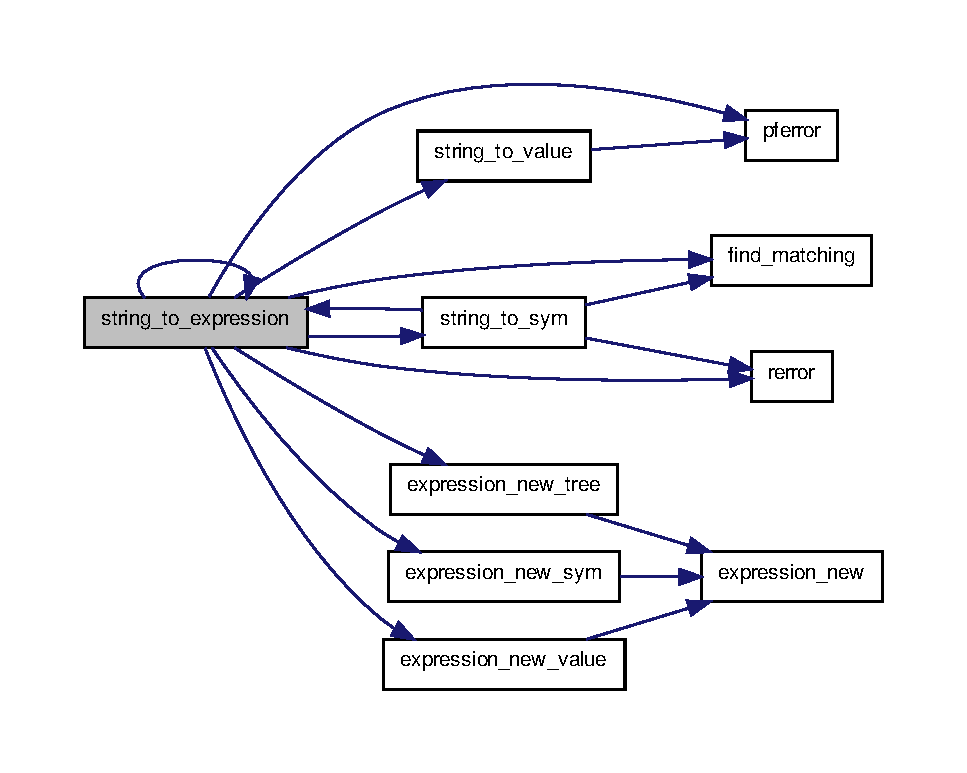
\includegraphics[width=350pt]{expression_8c_a63988c00ace0261c4896f132f5f86fda_cgraph}
\end{center}
\end{figure}

\hypertarget{expression_8h}{\section{expression.\+h File Reference}
\label{expression_8h}\index{expression.\+h@{expression.\+h}}
}


A compact math expression engine.  


{\ttfamily \#include $<$stddef.\+h$>$}\\*
{\ttfamily \#include \char`\"{}types.\+h\char`\"{}}\\*
{\ttfamily \#include \char`\"{}symbolic.\+h\char`\"{}}\\*
{\ttfamily \#include \char`\"{}expression\+\_\+lite.\+h\char`\"{}}\\*
Include dependency graph for expression.\+h\+:\nopagebreak
\begin{figure}[H]
\begin{center}
\leavevmode
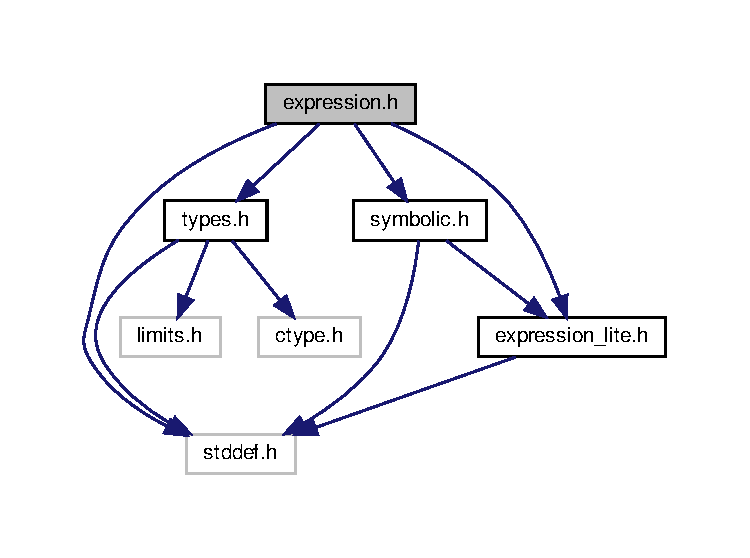
\includegraphics[width=350pt]{expression_8h__incl}
\end{center}
\end{figure}
\subsection*{Data Structures}
\begin{DoxyCompactItemize}
\item 
struct \hyperlink{structexpression__data__tree}{expression\+\_\+data\+\_\+tree}
\begin{DoxyCompactList}\small\item\em Expression data container for the expanded expression. \end{DoxyCompactList}\item 
union \hyperlink{unionexpression__data}{expression\+\_\+data}
\begin{DoxyCompactList}\small\item\em Expression data container. \end{DoxyCompactList}\item 
struct \hyperlink{structexpression}{expression}
\begin{DoxyCompactList}\small\item\em The stored representation of mathematical expressions. \end{DoxyCompactList}\end{DoxyCompactItemize}
\subsection*{Macros}
\begin{DoxyCompactItemize}
\item 
\#define \hyperlink{expression_8h_a153d42f7623b90824d99a93510e80065}{E\+X\+P\+\_\+\+B\+U\+F\+\_\+\+S\+I\+Z\+E}~256
\end{DoxyCompactItemize}
\subsection*{Typedefs}
\begin{DoxyCompactItemize}
\item 
typedef char \hyperlink{expression_8h_a3a229f715c187e4c6aede8af4779a858}{exp\+\_\+buf} \mbox{[}\hyperlink{expression_8h_a153d42f7623b90824d99a93510e80065}{E\+X\+P\+\_\+\+B\+U\+F\+\_\+\+S\+I\+Z\+E}\mbox{]}
\end{DoxyCompactItemize}
\subsection*{Enumerations}
\begin{DoxyCompactItemize}
\item 
enum \hyperlink{expression_8h_a5a6601c4e142145f0e87051cb21ece0f}{expression\+\_\+type} \{ \hyperlink{expression_8h_a5a6601c4e142145f0e87051cb21ece0fae6147a045f91d12b13e5b1be980f0c14}{E\+X\+P\+\_\+\+V\+A\+L\+U\+E}, 
\hyperlink{expression_8h_a5a6601c4e142145f0e87051cb21ece0fa85110f7c9b08f397c34d0a1b8111ef1b}{E\+X\+P\+\_\+\+T\+R\+E\+E}, 
\hyperlink{expression_8h_a5a6601c4e142145f0e87051cb21ece0fa7d51b8667dc755088ff87f371e427d96}{E\+X\+P\+\_\+\+S\+Y\+M\+B\+O\+L\+I\+C}
 \}
\begin{DoxyCompactList}\small\item\em Expression types. \end{DoxyCompactList}\end{DoxyCompactItemize}
\subsection*{Functions}
\begin{DoxyCompactItemize}
\item 
\hyperlink{expression__lite_8h_ac198bce62637e5d742da0218d544a7ac}{expression\+\_\+t} \hyperlink{expression_8h_a513e1cb7ae9dbcef50307f2c13e00dd9}{expression\+\_\+new} (void)
\begin{DoxyCompactList}\small\item\em New blank expression. \end{DoxyCompactList}\item 
\hyperlink{expression__lite_8h_ac198bce62637e5d742da0218d544a7ac}{expression\+\_\+t} \hyperlink{expression_8h_a7c44bf0c0e78a10270eeec18a89eb340}{expression\+\_\+new\+\_\+value} (\hyperlink{types_8h_ae4d4f561b975159d5852cb2c30bf20ef}{value\+\_\+t} val)
\item 
\hyperlink{expression__lite_8h_ac198bce62637e5d742da0218d544a7ac}{expression\+\_\+t} \hyperlink{expression_8h_affb6adb350cc9126e06af303607ca812}{expression\+\_\+new\+\_\+tree} (char op, \hyperlink{expression__lite_8h_ac198bce62637e5d742da0218d544a7ac}{expression\+\_\+t} left, \hyperlink{expression__lite_8h_ac198bce62637e5d742da0218d544a7ac}{expression\+\_\+t} right)
\item 
\hyperlink{expression__lite_8h_ac198bce62637e5d742da0218d544a7ac}{expression\+\_\+t} \hyperlink{expression_8h_a02b7142f5701d82971d1f21ec20772be}{expression\+\_\+new\+\_\+sym} (\hyperlink{symbolic_8h_a32ce0f63fa539078e25332dae6b7c77c}{sym\+\_\+t} \hyperlink{structsym}{sym})
\item 
void \hyperlink{expression_8h_a6f1cc930ee50ba61adf466fbdf4b1fb2}{expression\+\_\+free} (\hyperlink{expression__lite_8h_ac198bce62637e5d742da0218d544a7ac}{expression\+\_\+t} exp)
\begin{DoxyCompactList}\small\item\em Free an expression. \end{DoxyCompactList}\item 
\hyperlink{types_8h_ae4d4f561b975159d5852cb2c30bf20ef}{value\+\_\+t} \hyperlink{expression_8h_a70f3326a088855f6916f04baf27feed3}{expression\+\_\+evaluate} (\hyperlink{expression__lite_8h_ac198bce62637e5d742da0218d544a7ac}{expression\+\_\+t} exp)
\item 
void \hyperlink{expression_8h_aca3bb6ea526afbf4f238a0877fe3e131}{expression\+\_\+to\+\_\+string} (char $\ast$dst\+\_\+str, \hyperlink{expression__lite_8h_ac198bce62637e5d742da0218d544a7ac}{expression\+\_\+t} src\+\_\+exp)
\begin{DoxyCompactList}\small\item\em Expression to String. \end{DoxyCompactList}\item 
\hyperlink{expression__lite_8h_ac198bce62637e5d742da0218d544a7ac}{expression\+\_\+t} \hyperlink{expression_8h_a63988c00ace0261c4896f132f5f86fda}{string\+\_\+to\+\_\+expression} (size\+\_\+t str\+\_\+len, char const $\ast$str)
\begin{DoxyCompactList}\small\item\em Convert String to an Expression. \end{DoxyCompactList}\end{DoxyCompactItemize}


\subsection{Detailed Description}
A compact math expression engine. 

\begin{DoxyDate}{Date}
Apr 6, 2014 
\end{DoxyDate}
\begin{DoxyAuthor}{Author}
Craig Hesling 
\end{DoxyAuthor}


\subsection{Macro Definition Documentation}
\hypertarget{expression_8h_a153d42f7623b90824d99a93510e80065}{\index{expression.\+h@{expression.\+h}!E\+X\+P\+\_\+\+B\+U\+F\+\_\+\+S\+I\+Z\+E@{E\+X\+P\+\_\+\+B\+U\+F\+\_\+\+S\+I\+Z\+E}}
\index{E\+X\+P\+\_\+\+B\+U\+F\+\_\+\+S\+I\+Z\+E@{E\+X\+P\+\_\+\+B\+U\+F\+\_\+\+S\+I\+Z\+E}!expression.\+h@{expression.\+h}}
\subsubsection[{E\+X\+P\+\_\+\+B\+U\+F\+\_\+\+S\+I\+Z\+E}]{\setlength{\rightskip}{0pt plus 5cm}\#define E\+X\+P\+\_\+\+B\+U\+F\+\_\+\+S\+I\+Z\+E~256}}\label{expression_8h_a153d42f7623b90824d99a93510e80065}


\subsection{Typedef Documentation}
\hypertarget{expression_8h_a3a229f715c187e4c6aede8af4779a858}{\index{expression.\+h@{expression.\+h}!exp\+\_\+buf@{exp\+\_\+buf}}
\index{exp\+\_\+buf@{exp\+\_\+buf}!expression.\+h@{expression.\+h}}
\subsubsection[{exp\+\_\+buf}]{\setlength{\rightskip}{0pt plus 5cm}typedef char exp\+\_\+buf\mbox{[}{\bf E\+X\+P\+\_\+\+B\+U\+F\+\_\+\+S\+I\+Z\+E}\mbox{]}}}\label{expression_8h_a3a229f715c187e4c6aede8af4779a858}


\subsection{Enumeration Type Documentation}
\hypertarget{expression_8h_a5a6601c4e142145f0e87051cb21ece0f}{\index{expression.\+h@{expression.\+h}!expression\+\_\+type@{expression\+\_\+type}}
\index{expression\+\_\+type@{expression\+\_\+type}!expression.\+h@{expression.\+h}}
\subsubsection[{expression\+\_\+type}]{\setlength{\rightskip}{0pt plus 5cm}enum {\bf expression\+\_\+type}}}\label{expression_8h_a5a6601c4e142145f0e87051cb21ece0f}


Expression types. 

This is an enumeration of \hyperlink{expression__lite_8h_ac198bce62637e5d742da0218d544a7ac}{expression\+\_\+t}'s types. Specific types correspond to specific data containers in \hyperlink{unionexpression__data}{expression\+\_\+data}. \begin{Desc}
\item[Enumerator]\par
\begin{description}
\index{E\+X\+P\+\_\+\+V\+A\+L\+U\+E@{E\+X\+P\+\_\+\+V\+A\+L\+U\+E}!expression.\+h@{expression.\+h}}\index{expression.\+h@{expression.\+h}!E\+X\+P\+\_\+\+V\+A\+L\+U\+E@{E\+X\+P\+\_\+\+V\+A\+L\+U\+E}}\item[{\em 
\hypertarget{expression_8h_a5a6601c4e142145f0e87051cb21ece0fae6147a045f91d12b13e5b1be980f0c14}{E\+X\+P\+\_\+\+V\+A\+L\+U\+E}\label{expression_8h_a5a6601c4e142145f0e87051cb21ece0fae6147a045f91d12b13e5b1be980f0c14}
}]Contains a simple numeric values and undefines. \index{E\+X\+P\+\_\+\+T\+R\+E\+E@{E\+X\+P\+\_\+\+T\+R\+E\+E}!expression.\+h@{expression.\+h}}\index{expression.\+h@{expression.\+h}!E\+X\+P\+\_\+\+T\+R\+E\+E@{E\+X\+P\+\_\+\+T\+R\+E\+E}}\item[{\em 
\hypertarget{expression_8h_a5a6601c4e142145f0e87051cb21ece0fa85110f7c9b08f397c34d0a1b8111ef1b}{E\+X\+P\+\_\+\+T\+R\+E\+E}\label{expression_8h_a5a6601c4e142145f0e87051cb21ece0fa85110f7c9b08f397c34d0a1b8111ef1b}
}]An expression over an operation and sub-\/expression. \index{E\+X\+P\+\_\+\+S\+Y\+M\+B\+O\+L\+I\+C@{E\+X\+P\+\_\+\+S\+Y\+M\+B\+O\+L\+I\+C}!expression.\+h@{expression.\+h}}\index{expression.\+h@{expression.\+h}!E\+X\+P\+\_\+\+S\+Y\+M\+B\+O\+L\+I\+C@{E\+X\+P\+\_\+\+S\+Y\+M\+B\+O\+L\+I\+C}}\item[{\em 
\hypertarget{expression_8h_a5a6601c4e142145f0e87051cb21ece0fa7d51b8667dc755088ff87f371e427d96}{E\+X\+P\+\_\+\+S\+Y\+M\+B\+O\+L\+I\+C}\label{expression_8h_a5a6601c4e142145f0e87051cb21ece0fa7d51b8667dc755088ff87f371e427d96}
}]Symbolic named references. \end{description}
\end{Desc}


\subsection{Function Documentation}
\hypertarget{expression_8h_a70f3326a088855f6916f04baf27feed3}{\index{expression.\+h@{expression.\+h}!expression\+\_\+evaluate@{expression\+\_\+evaluate}}
\index{expression\+\_\+evaluate@{expression\+\_\+evaluate}!expression.\+h@{expression.\+h}}
\subsubsection[{expression\+\_\+evaluate}]{\setlength{\rightskip}{0pt plus 5cm}{\bf value\+\_\+t} expression\+\_\+evaluate (
\begin{DoxyParamCaption}
\item[{{\bf expression\+\_\+t}}]{exp}
\end{DoxyParamCaption}
)}}\label{expression_8h_a70f3326a088855f6916f04baf27feed3}
\hypertarget{expression_8h_a6f1cc930ee50ba61adf466fbdf4b1fb2}{\index{expression.\+h@{expression.\+h}!expression\+\_\+free@{expression\+\_\+free}}
\index{expression\+\_\+free@{expression\+\_\+free}!expression.\+h@{expression.\+h}}
\subsubsection[{expression\+\_\+free}]{\setlength{\rightskip}{0pt plus 5cm}void expression\+\_\+free (
\begin{DoxyParamCaption}
\item[{{\bf expression\+\_\+t}}]{exp}
\end{DoxyParamCaption}
)}}\label{expression_8h_a6f1cc930ee50ba61adf466fbdf4b1fb2}


Free an expression. 


\begin{DoxyParams}{Parameters}
{\em exp} & The expression to free \\
\hline
\end{DoxyParams}
\hypertarget{expression_8h_a513e1cb7ae9dbcef50307f2c13e00dd9}{\index{expression.\+h@{expression.\+h}!expression\+\_\+new@{expression\+\_\+new}}
\index{expression\+\_\+new@{expression\+\_\+new}!expression.\+h@{expression.\+h}}
\subsubsection[{expression\+\_\+new}]{\setlength{\rightskip}{0pt plus 5cm}{\bf expression\+\_\+t} expression\+\_\+new (
\begin{DoxyParamCaption}
\item[{void}]{}
\end{DoxyParamCaption}
)}}\label{expression_8h_a513e1cb7ae9dbcef50307f2c13e00dd9}


New blank expression. 

This function creates the most basic empty expression. \begin{DoxyReturn}{Returns}
A new empty expression 
\end{DoxyReturn}
\hypertarget{expression_8h_a02b7142f5701d82971d1f21ec20772be}{\index{expression.\+h@{expression.\+h}!expression\+\_\+new\+\_\+sym@{expression\+\_\+new\+\_\+sym}}
\index{expression\+\_\+new\+\_\+sym@{expression\+\_\+new\+\_\+sym}!expression.\+h@{expression.\+h}}
\subsubsection[{expression\+\_\+new\+\_\+sym}]{\setlength{\rightskip}{0pt plus 5cm}{\bf expression\+\_\+t} expression\+\_\+new\+\_\+sym (
\begin{DoxyParamCaption}
\item[{{\bf sym\+\_\+t}}]{sym}
\end{DoxyParamCaption}
)}}\label{expression_8h_a02b7142f5701d82971d1f21ec20772be}


Here is the call graph for this function\+:\nopagebreak
\begin{figure}[H]
\begin{center}
\leavevmode
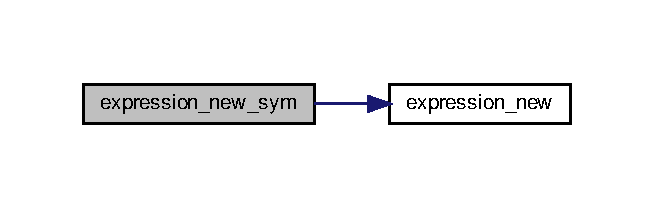
\includegraphics[width=316pt]{expression_8h_a02b7142f5701d82971d1f21ec20772be_cgraph}
\end{center}
\end{figure}


\hypertarget{expression_8h_affb6adb350cc9126e06af303607ca812}{\index{expression.\+h@{expression.\+h}!expression\+\_\+new\+\_\+tree@{expression\+\_\+new\+\_\+tree}}
\index{expression\+\_\+new\+\_\+tree@{expression\+\_\+new\+\_\+tree}!expression.\+h@{expression.\+h}}
\subsubsection[{expression\+\_\+new\+\_\+tree}]{\setlength{\rightskip}{0pt plus 5cm}{\bf expression\+\_\+t} expression\+\_\+new\+\_\+tree (
\begin{DoxyParamCaption}
\item[{char}]{op, }
\item[{{\bf expression\+\_\+t}}]{left, }
\item[{{\bf expression\+\_\+t}}]{right}
\end{DoxyParamCaption}
)}}\label{expression_8h_affb6adb350cc9126e06af303607ca812}


Here is the call graph for this function\+:\nopagebreak
\begin{figure}[H]
\begin{center}
\leavevmode
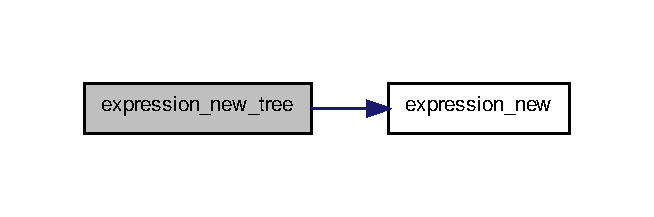
\includegraphics[width=314pt]{expression_8h_affb6adb350cc9126e06af303607ca812_cgraph}
\end{center}
\end{figure}


\hypertarget{expression_8h_a7c44bf0c0e78a10270eeec18a89eb340}{\index{expression.\+h@{expression.\+h}!expression\+\_\+new\+\_\+value@{expression\+\_\+new\+\_\+value}}
\index{expression\+\_\+new\+\_\+value@{expression\+\_\+new\+\_\+value}!expression.\+h@{expression.\+h}}
\subsubsection[{expression\+\_\+new\+\_\+value}]{\setlength{\rightskip}{0pt plus 5cm}{\bf expression\+\_\+t} expression\+\_\+new\+\_\+value (
\begin{DoxyParamCaption}
\item[{{\bf value\+\_\+t}}]{val}
\end{DoxyParamCaption}
)}}\label{expression_8h_a7c44bf0c0e78a10270eeec18a89eb340}


Here is the call graph for this function\+:\nopagebreak
\begin{figure}[H]
\begin{center}
\leavevmode
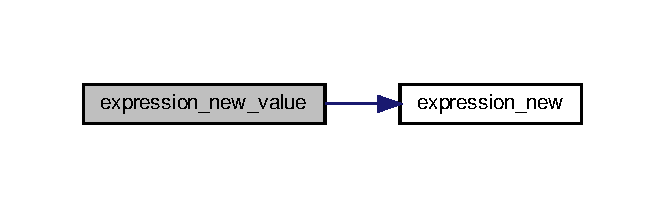
\includegraphics[width=320pt]{expression_8h_a7c44bf0c0e78a10270eeec18a89eb340_cgraph}
\end{center}
\end{figure}


\hypertarget{expression_8h_aca3bb6ea526afbf4f238a0877fe3e131}{\index{expression.\+h@{expression.\+h}!expression\+\_\+to\+\_\+string@{expression\+\_\+to\+\_\+string}}
\index{expression\+\_\+to\+\_\+string@{expression\+\_\+to\+\_\+string}!expression.\+h@{expression.\+h}}
\subsubsection[{expression\+\_\+to\+\_\+string}]{\setlength{\rightskip}{0pt plus 5cm}void expression\+\_\+to\+\_\+string (
\begin{DoxyParamCaption}
\item[{char $\ast$}]{dst\+\_\+str, }
\item[{{\bf expression\+\_\+t}}]{src\+\_\+exp}
\end{DoxyParamCaption}
)}}\label{expression_8h_aca3bb6ea526afbf4f238a0877fe3e131}


Expression to String. 

\hypertarget{expression_8h_a63988c00ace0261c4896f132f5f86fda}{\index{expression.\+h@{expression.\+h}!string\+\_\+to\+\_\+expression@{string\+\_\+to\+\_\+expression}}
\index{string\+\_\+to\+\_\+expression@{string\+\_\+to\+\_\+expression}!expression.\+h@{expression.\+h}}
\subsubsection[{string\+\_\+to\+\_\+expression}]{\setlength{\rightskip}{0pt plus 5cm}{\bf expression\+\_\+t} string\+\_\+to\+\_\+expression (
\begin{DoxyParamCaption}
\item[{size\+\_\+t}]{str\+\_\+len, }
\item[{char const $\ast$}]{str}
\end{DoxyParamCaption}
)}}\label{expression_8h_a63988c00ace0261c4896f132f5f86fda}


Convert String to an Expression. 

Parses a string into an expression. \begin{DoxyNote}{Note}
level was type int -\/ changed to unsigned to temporarily quiet compiler 
\end{DoxyNote}
\begin{DoxyRefDesc}{Bug}
\item[\hyperlink{bug__bug000001}{Bug}]Cannot parse negative numbers \begin{DoxyWarning}{Warning}
Symbols must start with A\+L\+P\+H\+A chars to be properly identified.
\end{DoxyWarning}
\end{DoxyRefDesc}
\hypertarget{expression__lite_8h_parsing_algorithm}{}\subsection{Algorithm}\label{expression__lite_8h_parsing_algorithm}
\hypertarget{expression__lite_8h_parsing_overview}{}\subsubsection{Parsing Overview}\label{expression__lite_8h_parsing_overview}

\begin{DoxyItemize}
\item Step 1\+: Recording details about the string while scanning from left to right.
\item Step 2\+: There are two real cases. The string is a single number (with no operations) or it is two sub-\/expressions joined by an operation.~\newline
 Cases\+:
\begin{DoxyItemize}
\item If it is a simple number, we know how to parse it and create a value expression.
\item If it is not just a number, we want split the string about the operation at the lowest level. (in practice, we end up finding the one that is farthest left of the lowest level) We then construct a tree expression with the chosen operation and the sub-\/expression results from running the function recursively on each of the sub-\/strings.
\end{DoxyItemize}
\end{DoxyItemize}


\begin{DoxyParams}{Parameters}
{\em str\+\_\+len} & Length of given string \\
\hline
{\em str} & String to parse \\
\hline
\end{DoxyParams}
\begin{DoxyReturn}{Returns}
The expression\+\_\+t representation of the inputed string
\end{DoxyReturn}
\begin{DoxyRefDesc}{Test}
\item[\hyperlink{test__test000001}{Test}]Test for negative values \end{DoxyRefDesc}
\begin{DoxyRefDesc}{Todo}
\item[\hyperlink{todo__todo000001}{Todo}]Allow symbols to be detected when they start with numeric digits also. \hyperlink{symbolic_8h_a78aa047f421c2d8ab5fab3c72d123d1b}{string\+\_\+to\+\_\+sym} is already compatible. \end{DoxyRefDesc}


$<$ Store original index

$<$ Used to explore the presence of a symbol parameter

\begin{DoxyRefDesc}{Todo}
\item[\hyperlink{todo__todo000002}{Todo}]Do series of additional syntax checks here. \end{DoxyRefDesc}
\begin{DoxyRefDesc}{Todo}
\item[\hyperlink{todo__todo000003}{Todo}]Syntax Check\+: Check that level==0 \end{DoxyRefDesc}
\begin{DoxyRefDesc}{Todo}
\item[\hyperlink{todo__todo000004}{Todo}]Syntax Check\+: Check that oparen\+\_\+count==cparen\+\_\+count \end{DoxyRefDesc}


\begin{DoxyNote}{Note}
left\+\_\+buf and right\+\_\+buf were changed to use malloc to avoid errors with C90 compilers 
\end{DoxyNote}

\hypertarget{expression__lite_8h}{}\section{expression\+\_\+lite.\+h File Reference}
\label{expression__lite_8h}\index{expression\+\_\+lite.\+h@{expression\+\_\+lite.\+h}}
{\ttfamily \#include $<$stddef.\+h$>$}\newline
Include dependency graph for expression\+\_\+lite.\+h\+:
\nopagebreak
\begin{figure}[H]
\begin{center}
\leavevmode
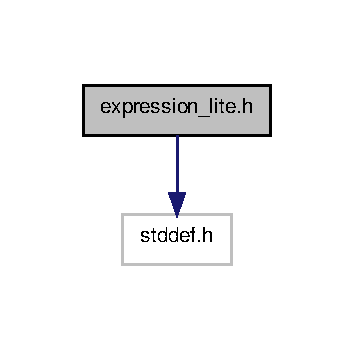
\includegraphics[width=170pt]{expression__lite_8h__incl}
\end{center}
\end{figure}
\subsection*{Typedefs}
\begin{DoxyCompactItemize}
\item 
typedef struct \hyperlink{structexpression}{expression} $\ast$ \hyperlink{expression__lite_8h_ac198bce62637e5d742da0218d544a7ac}{expression\+\_\+t}
\end{DoxyCompactItemize}
\subsection*{Functions}
\begin{DoxyCompactItemize}
\item 
\hyperlink{expression__lite_8h_ac198bce62637e5d742da0218d544a7ac}{expression\+\_\+t} \hyperlink{expression__lite_8h_a513e1cb7ae9dbcef50307f2c13e00dd9}{expression\+\_\+new} (void)
\begin{DoxyCompactList}\small\item\em New blank expression. \end{DoxyCompactList}\item 
void \hyperlink{expression__lite_8h_a6f1cc930ee50ba61adf466fbdf4b1fb2}{expression\+\_\+free} (\hyperlink{expression__lite_8h_ac198bce62637e5d742da0218d544a7ac}{expression\+\_\+t} exp)
\begin{DoxyCompactList}\small\item\em Free an expression. \end{DoxyCompactList}\item 
\hyperlink{types_8h_ae4d4f561b975159d5852cb2c30bf20ef}{value\+\_\+t} \hyperlink{expression__lite_8h_a70f3326a088855f6916f04baf27feed3}{expression\+\_\+evaluate} (\hyperlink{expression__lite_8h_ac198bce62637e5d742da0218d544a7ac}{expression\+\_\+t} exp)
\item 
void \hyperlink{expression__lite_8h_aca3bb6ea526afbf4f238a0877fe3e131}{expression\+\_\+to\+\_\+string} (char $\ast$dst\+\_\+str, \hyperlink{expression__lite_8h_ac198bce62637e5d742da0218d544a7ac}{expression\+\_\+t} src\+\_\+exp)
\begin{DoxyCompactList}\small\item\em Expression to String. \end{DoxyCompactList}\item 
\hyperlink{expression__lite_8h_ac198bce62637e5d742da0218d544a7ac}{expression\+\_\+t} \hyperlink{expression__lite_8h_a63988c00ace0261c4896f132f5f86fda}{string\+\_\+to\+\_\+expression} (size\+\_\+t str\+\_\+len, char const $\ast$str)
\begin{DoxyCompactList}\small\item\em Convert String to an Expression. \end{DoxyCompactList}\end{DoxyCompactItemize}


\subsection{Detailed Description}
\begin{DoxyDate}{Date}
May 3, 2014 
\end{DoxyDate}
\begin{DoxyAuthor}{Author}
Craig Hesling
\end{DoxyAuthor}
Does not include any other project header file. This ensures that there are no circular dependencies. 

\subsection{Typedef Documentation}
\mbox{\Hypertarget{expression__lite_8h_ac198bce62637e5d742da0218d544a7ac}\label{expression__lite_8h_ac198bce62637e5d742da0218d544a7ac}} 
\index{expression\+\_\+lite.\+h@{expression\+\_\+lite.\+h}!expression\+\_\+t@{expression\+\_\+t}}
\index{expression\+\_\+t@{expression\+\_\+t}!expression\+\_\+lite.\+h@{expression\+\_\+lite.\+h}}
\subsubsection{\texorpdfstring{expression\+\_\+t}{expression\_t}}
{\footnotesize\ttfamily typedef struct \hyperlink{structexpression}{expression}$\ast$ \hyperlink{expression__lite_8h_ac198bce62637e5d742da0218d544a7ac}{expression\+\_\+t}}



\subsection{Function Documentation}
\mbox{\Hypertarget{expression__lite_8h_a70f3326a088855f6916f04baf27feed3}\label{expression__lite_8h_a70f3326a088855f6916f04baf27feed3}} 
\index{expression\+\_\+lite.\+h@{expression\+\_\+lite.\+h}!expression\+\_\+evaluate@{expression\+\_\+evaluate}}
\index{expression\+\_\+evaluate@{expression\+\_\+evaluate}!expression\+\_\+lite.\+h@{expression\+\_\+lite.\+h}}
\subsubsection{\texorpdfstring{expression\+\_\+evaluate()}{expression\_evaluate()}}
{\footnotesize\ttfamily \hyperlink{types_8h_ae4d4f561b975159d5852cb2c30bf20ef}{value\+\_\+t} expression\+\_\+evaluate (\begin{DoxyParamCaption}\item[{\hyperlink{expression__lite_8h_ac198bce62637e5d742da0218d544a7ac}{expression\+\_\+t}}]{exp }\end{DoxyParamCaption})}

Here is the call graph for this function\+:
\nopagebreak
\begin{figure}[H]
\begin{center}
\leavevmode
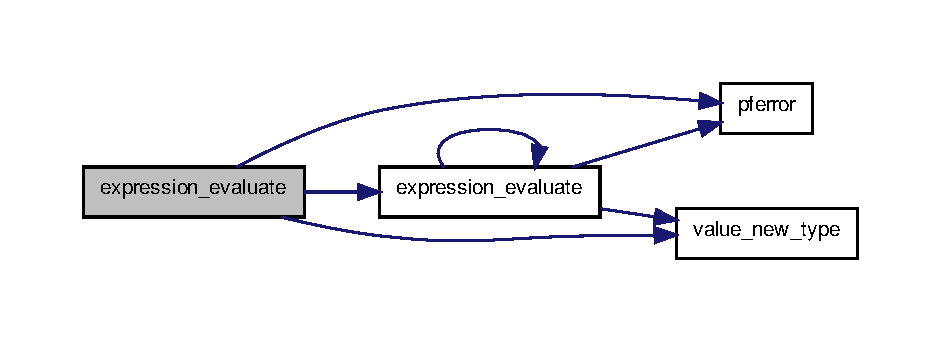
\includegraphics[width=350pt]{expression__lite_8h_a70f3326a088855f6916f04baf27feed3_cgraph}
\end{center}
\end{figure}
\mbox{\Hypertarget{expression__lite_8h_a6f1cc930ee50ba61adf466fbdf4b1fb2}\label{expression__lite_8h_a6f1cc930ee50ba61adf466fbdf4b1fb2}} 
\index{expression\+\_\+lite.\+h@{expression\+\_\+lite.\+h}!expression\+\_\+free@{expression\+\_\+free}}
\index{expression\+\_\+free@{expression\+\_\+free}!expression\+\_\+lite.\+h@{expression\+\_\+lite.\+h}}
\subsubsection{\texorpdfstring{expression\+\_\+free()}{expression\_free()}}
{\footnotesize\ttfamily void expression\+\_\+free (\begin{DoxyParamCaption}\item[{\hyperlink{expression__lite_8h_ac198bce62637e5d742da0218d544a7ac}{expression\+\_\+t}}]{exp }\end{DoxyParamCaption})}



Free an expression. 


\begin{DoxyParams}{Parameters}
{\em exp} & The expression to free \\
\hline
\end{DoxyParams}
Here is the call graph for this function\+:
\nopagebreak
\begin{figure}[H]
\begin{center}
\leavevmode
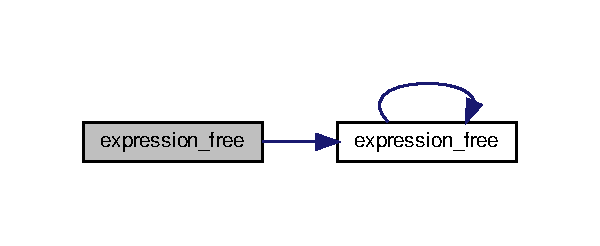
\includegraphics[width=288pt]{expression__lite_8h_a6f1cc930ee50ba61adf466fbdf4b1fb2_cgraph}
\end{center}
\end{figure}
\mbox{\Hypertarget{expression__lite_8h_a513e1cb7ae9dbcef50307f2c13e00dd9}\label{expression__lite_8h_a513e1cb7ae9dbcef50307f2c13e00dd9}} 
\index{expression\+\_\+lite.\+h@{expression\+\_\+lite.\+h}!expression\+\_\+new@{expression\+\_\+new}}
\index{expression\+\_\+new@{expression\+\_\+new}!expression\+\_\+lite.\+h@{expression\+\_\+lite.\+h}}
\subsubsection{\texorpdfstring{expression\+\_\+new()}{expression\_new()}}
{\footnotesize\ttfamily \hyperlink{expression__lite_8h_ac198bce62637e5d742da0218d544a7ac}{expression\+\_\+t} expression\+\_\+new (\begin{DoxyParamCaption}\item[{void}]{ }\end{DoxyParamCaption})}



New blank expression. 

This function creates the most basic empty expression. \begin{DoxyReturn}{Returns}
A new empty expression 
\end{DoxyReturn}
\mbox{\Hypertarget{expression__lite_8h_aca3bb6ea526afbf4f238a0877fe3e131}\label{expression__lite_8h_aca3bb6ea526afbf4f238a0877fe3e131}} 
\index{expression\+\_\+lite.\+h@{expression\+\_\+lite.\+h}!expression\+\_\+to\+\_\+string@{expression\+\_\+to\+\_\+string}}
\index{expression\+\_\+to\+\_\+string@{expression\+\_\+to\+\_\+string}!expression\+\_\+lite.\+h@{expression\+\_\+lite.\+h}}
\subsubsection{\texorpdfstring{expression\+\_\+to\+\_\+string()}{expression\_to\_string()}}
{\footnotesize\ttfamily void expression\+\_\+to\+\_\+string (\begin{DoxyParamCaption}\item[{char $\ast$}]{dst\+\_\+str,  }\item[{\hyperlink{expression__lite_8h_ac198bce62637e5d742da0218d544a7ac}{expression\+\_\+t}}]{src\+\_\+exp }\end{DoxyParamCaption})}



Expression to String. 

Here is the call graph for this function\+:
\nopagebreak
\begin{figure}[H]
\begin{center}
\leavevmode
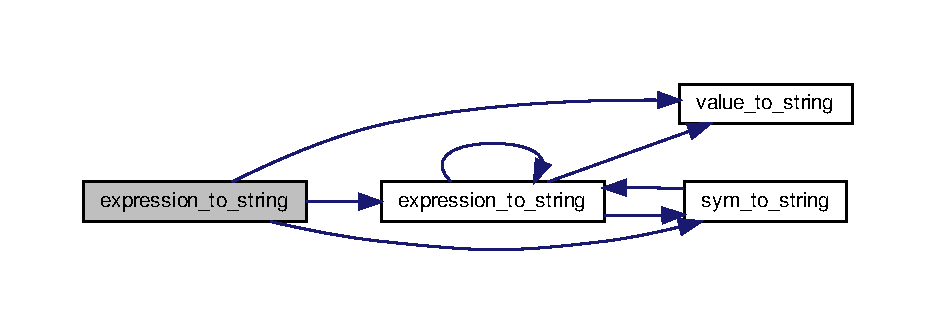
\includegraphics[width=350pt]{expression__lite_8h_aca3bb6ea526afbf4f238a0877fe3e131_cgraph}
\end{center}
\end{figure}
\mbox{\Hypertarget{expression__lite_8h_a63988c00ace0261c4896f132f5f86fda}\label{expression__lite_8h_a63988c00ace0261c4896f132f5f86fda}} 
\index{expression\+\_\+lite.\+h@{expression\+\_\+lite.\+h}!string\+\_\+to\+\_\+expression@{string\+\_\+to\+\_\+expression}}
\index{string\+\_\+to\+\_\+expression@{string\+\_\+to\+\_\+expression}!expression\+\_\+lite.\+h@{expression\+\_\+lite.\+h}}
\subsubsection{\texorpdfstring{string\+\_\+to\+\_\+expression()}{string\_to\_expression()}}
{\footnotesize\ttfamily \hyperlink{expression__lite_8h_ac198bce62637e5d742da0218d544a7ac}{expression\+\_\+t} string\+\_\+to\+\_\+expression (\begin{DoxyParamCaption}\item[{size\+\_\+t}]{str\+\_\+len,  }\item[{char const $\ast$}]{str }\end{DoxyParamCaption})}



Convert String to an Expression. 

Parses a string into an expression. \begin{DoxyNote}{Note}
level was type int -\/ changed to unsigned to temporarily quiet compiler 
\end{DoxyNote}
\begin{DoxyRefDesc}{Bug}
\item[\hyperlink{bug__bug000001}{Bug}]Cannot parse negative numbers \end{DoxyRefDesc}
\begin{DoxyWarning}{Warning}
Symbols must start with A\+L\+P\+HA chars to be properly identified.
\end{DoxyWarning}
\hypertarget{expression__lite_8h_parsing_algorithm}{}\subsection{Algorithm}\label{expression__lite_8h_parsing_algorithm}
\hypertarget{expression__lite_8h_parsing_overview}{}\subsubsection{Parsing Overview}\label{expression__lite_8h_parsing_overview}

\begin{DoxyItemize}
\item Step 1\+: Recording details about the string while scanning from left to right.
\item Step 2\+: There are two real cases. The string is a single number (with no operations) or it is two sub-\/expressions joined by an operation.~\newline
 Cases\+:
\begin{DoxyItemize}
\item If it is a simple number, we know how to parse it and create a value expression.
\item If it is not just a number, we want split the string about the operation at the lowest level. (in practice, we end up finding the one that is farthest left of the lowest level) We then construct a tree expression with the chosen operation and the sub-\/expression results from running the function recursively on each of the sub-\/strings.
\end{DoxyItemize}
\end{DoxyItemize}


\begin{DoxyParams}{Parameters}
{\em str\+\_\+len} & Length of given string \\
\hline
{\em str} & String to parse \\
\hline
\end{DoxyParams}
\begin{DoxyReturn}{Returns}
The expression\+\_\+t representation of the inputed string
\end{DoxyReturn}
\begin{DoxyRefDesc}{Test}
\item[\hyperlink{test__test000001}{Test}]Test for negative values \end{DoxyRefDesc}
\begin{DoxyRefDesc}{Todo}
\item[\hyperlink{todo__todo000001}{Todo}]Allow symbols to be detected when they start with numeric digits also. \hyperlink{symbolic_8h_a78aa047f421c2d8ab5fab3c72d123d1b}{string\+\_\+to\+\_\+sym} is already compatible. \end{DoxyRefDesc}


$<$ Store original index

$<$ Used to explore the presence of a symbol parameter

\begin{DoxyRefDesc}{Todo}
\item[\hyperlink{todo__todo000002}{Todo}]Do series of additional syntax checks here. \end{DoxyRefDesc}
\begin{DoxyRefDesc}{Todo}
\item[\hyperlink{todo__todo000003}{Todo}]Syntax Check\+: Check that level==0 \end{DoxyRefDesc}
\begin{DoxyRefDesc}{Todo}
\item[\hyperlink{todo__todo000004}{Todo}]Syntax Check\+: Check that oparen\+\_\+count==cparen\+\_\+count \end{DoxyRefDesc}


\begin{DoxyNote}{Note}
left\+\_\+buf and right\+\_\+buf were changed to use malloc to avoid errors with C90 compilers 
\end{DoxyNote}
Here is the call graph for this function\+:
\nopagebreak
\begin{figure}[H]
\begin{center}
\leavevmode
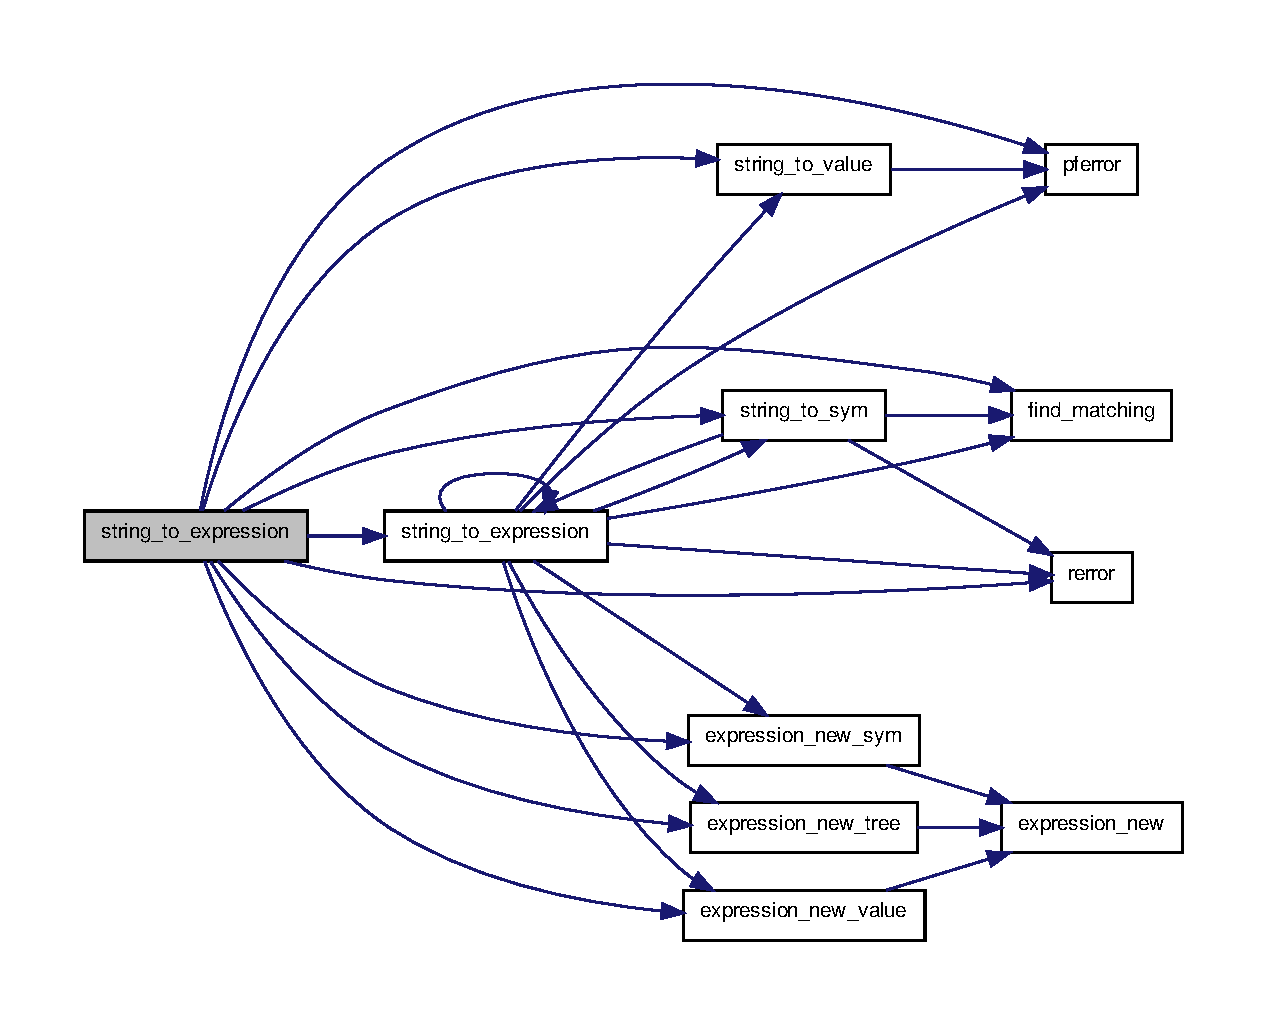
\includegraphics[width=350pt]{expression__lite_8h_a63988c00ace0261c4896f132f5f86fda_cgraph}
\end{center}
\end{figure}

\hypertarget{main_8c}{\section{main.\+c File Reference}
\label{main_8c}\index{main.\+c@{main.\+c}}
}
{\ttfamily \#include $<$stdio.\+h$>$}\\*
{\ttfamily \#include $<$stdlib.\+h$>$}\\*
{\ttfamily \#include $<$assert.\+h$>$}\\*
{\ttfamily \#include $<$string.\+h$>$}\\*
{\ttfamily \#include \char`\"{}errors.\+h\char`\"{}}\\*
{\ttfamily \#include \char`\"{}types.\+h\char`\"{}}\\*
{\ttfamily \#include \char`\"{}workspace.\+h\char`\"{}}\\*
{\ttfamily \#include \char`\"{}expression.\+h\char`\"{}}\\*
Include dependency graph for main.\+c\+:\nopagebreak
\begin{figure}[H]
\begin{center}
\leavevmode
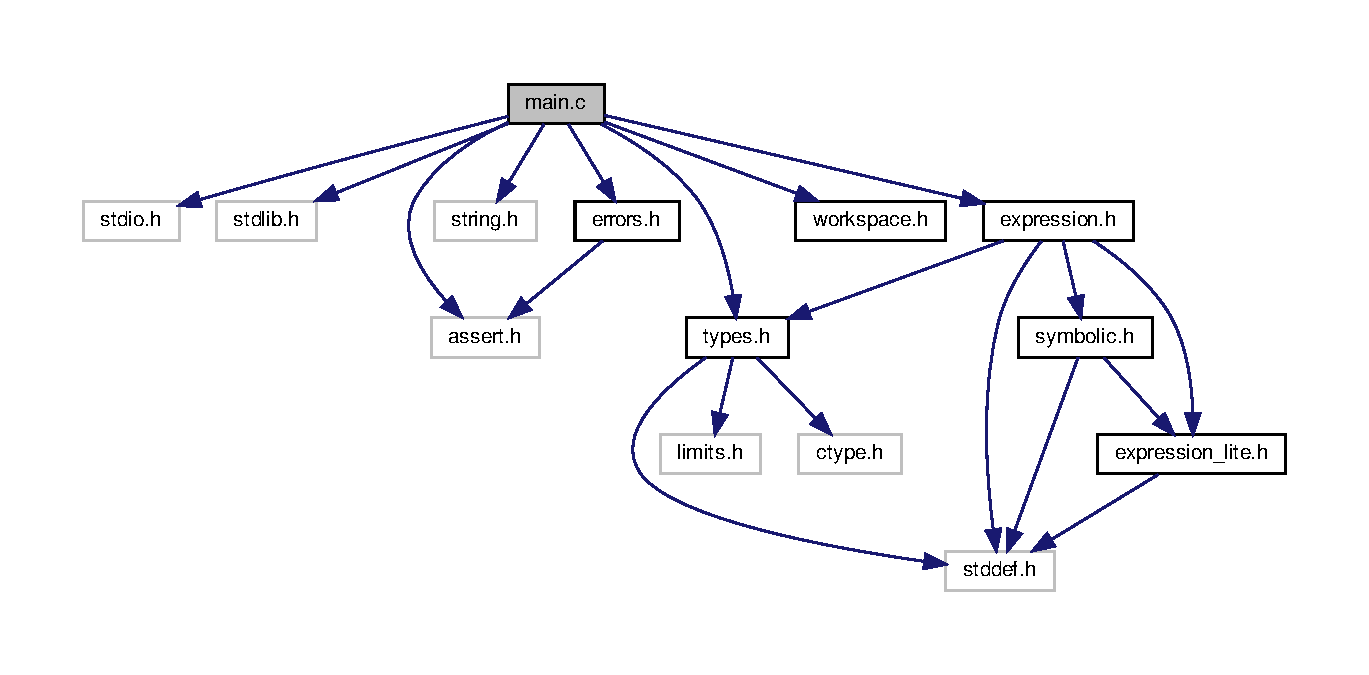
\includegraphics[width=350pt]{main_8c__incl}
\end{center}
\end{figure}
\subsection*{Macros}
\begin{DoxyCompactItemize}
\item 
\#define \hyperlink{main_8c_a7b3b25cba33b07c303f3060fe41887f6}{B\+L\+A\+C\+K}~30
\item 
\#define \hyperlink{main_8c_a8d23feea868a983c8c2b661e1e16972f}{R\+E\+D}~31
\item 
\#define \hyperlink{main_8c_acfbc006ea433ad708fdee3e82996e721}{G\+R\+E\+E\+N}~32
\item 
\#define \hyperlink{main_8c_abf681265909adf3d3e8116c93c0ba179}{Y\+E\+L\+L\+O\+W}~33
\item 
\#define \hyperlink{main_8c_a79d10e672abb49ad63eeaa8aaef57c38}{B\+L\+U\+E}~34
\item 
\#define \hyperlink{main_8c_a0bb0b009e7a7390473ace4d98bd843c0}{P\+U\+R\+P\+L\+E}~35
\item 
\#define \hyperlink{main_8c_a03e7881ce42823bcd8c3e798e03e7507}{T\+E\+A\+L}~36
\item 
\#define \hyperlink{main_8c_adce122f566c88a1eceeb79a635afa964}{G\+R\+E\+Y}~37
\item 
\#define \hyperlink{main_8c_a87b537f5fa5c109d3c05c13d6b18f382}{W\+H\+I\+T\+E}~38
\item 
\#define \hyperlink{main_8c_a7b74f5293ac251b336817f016f37ef54}{x\+C\+O\+L\+O\+R}(color, str)~\char`\"{}\textbackslash{}033\mbox{[}\char`\"{}\#color\char`\"{}m\char`\"{}str\char`\"{}\textbackslash{}033\mbox{[}m\char`\"{}
\item 
\#define \hyperlink{main_8c_afcb295f230ec87303e40ae53267dc81f}{C\+O\+L\+O\+R}(color, str)~\hyperlink{main_8c_a7b74f5293ac251b336817f016f37ef54}{x\+C\+O\+L\+O\+R}(color, \#str)
\item 
\#define \hyperlink{main_8c_a63b91eaa0a70d50671e305c4f1603b53}{E\+X\+P\+E\+C\+T}(exp)~\hyperlink{main_8c_afcb295f230ec87303e40ae53267dc81f}{C\+O\+L\+O\+R}(\hyperlink{main_8c_acfbc006ea433ad708fdee3e82996e721}{G\+R\+E\+E\+N}, exp)
\item 
\#define \hyperlink{main_8c_ab6b4f9167f1d2de786d796d82f941454}{R\+E\+S\+U\+L\+T}(res)~\hyperlink{main_8c_afcb295f230ec87303e40ae53267dc81f}{C\+O\+L\+O\+R}(\hyperlink{main_8c_a0bb0b009e7a7390473ace4d98bd843c0}{P\+U\+R\+P\+L\+E}, res)
\end{DoxyCompactItemize}
\subsection*{Functions}
\begin{DoxyCompactItemize}
\item 
void \hyperlink{main_8c_ad7a5fe9ac7cb34a8455d013cc154283b}{rtests} (void)
\begin{DoxyCompactList}\small\item\em Random Tests. \end{DoxyCompactList}\item 
void \hyperlink{main_8c_a2b5008f0c056e4e83b3ead2c95e50297}{test0} (void)
\begin{DoxyCompactList}\small\item\em Tests \hyperlink{expression__lite_8h_aca3bb6ea526afbf4f238a0877fe3e131}{expression\+\_\+to\+\_\+string} and then \hyperlink{expression__lite_8h_a70f3326a088855f6916f04baf27feed3}{expression\+\_\+evaluate} functions. \end{DoxyCompactList}\item 
void \hyperlink{main_8c_a299e410e6033d409446bd27bd4fb5b90}{test1} (char $\ast$str)
\begin{DoxyCompactList}\small\item\em Tests \hyperlink{expression__lite_8h_a63988c00ace0261c4896f132f5f86fda}{string\+\_\+to\+\_\+expression} on the string argument and then tests \hyperlink{expression__lite_8h_aca3bb6ea526afbf4f238a0877fe3e131}{expression\+\_\+to\+\_\+string} on it's output. \end{DoxyCompactList}\item 
int \hyperlink{main_8c_a0ddf1224851353fc92bfbff6f499fa97}{main} (int argc, char $\ast$argv\mbox{[}$\,$\mbox{]})
\end{DoxyCompactItemize}


\subsection{Detailed Description}
\begin{DoxyDate}{Date}
Apr 6, 2014 
\end{DoxyDate}
\begin{DoxyAuthor}{Author}
Craig Hesling 
\end{DoxyAuthor}


\subsection{Macro Definition Documentation}
\hypertarget{main_8c_a7b3b25cba33b07c303f3060fe41887f6}{\index{main.\+c@{main.\+c}!B\+L\+A\+C\+K@{B\+L\+A\+C\+K}}
\index{B\+L\+A\+C\+K@{B\+L\+A\+C\+K}!main.\+c@{main.\+c}}
\subsubsection[{B\+L\+A\+C\+K}]{\setlength{\rightskip}{0pt plus 5cm}\#define B\+L\+A\+C\+K~30}}\label{main_8c_a7b3b25cba33b07c303f3060fe41887f6}
\hypertarget{main_8c_a79d10e672abb49ad63eeaa8aaef57c38}{\index{main.\+c@{main.\+c}!B\+L\+U\+E@{B\+L\+U\+E}}
\index{B\+L\+U\+E@{B\+L\+U\+E}!main.\+c@{main.\+c}}
\subsubsection[{B\+L\+U\+E}]{\setlength{\rightskip}{0pt plus 5cm}\#define B\+L\+U\+E~34}}\label{main_8c_a79d10e672abb49ad63eeaa8aaef57c38}
\hypertarget{main_8c_afcb295f230ec87303e40ae53267dc81f}{\index{main.\+c@{main.\+c}!C\+O\+L\+O\+R@{C\+O\+L\+O\+R}}
\index{C\+O\+L\+O\+R@{C\+O\+L\+O\+R}!main.\+c@{main.\+c}}
\subsubsection[{C\+O\+L\+O\+R}]{\setlength{\rightskip}{0pt plus 5cm}\#define C\+O\+L\+O\+R(
\begin{DoxyParamCaption}
\item[{}]{color, }
\item[{}]{str}
\end{DoxyParamCaption}
)~{\bf x\+C\+O\+L\+O\+R}(color, \#str)}}\label{main_8c_afcb295f230ec87303e40ae53267dc81f}
\hypertarget{main_8c_a63b91eaa0a70d50671e305c4f1603b53}{\index{main.\+c@{main.\+c}!E\+X\+P\+E\+C\+T@{E\+X\+P\+E\+C\+T}}
\index{E\+X\+P\+E\+C\+T@{E\+X\+P\+E\+C\+T}!main.\+c@{main.\+c}}
\subsubsection[{E\+X\+P\+E\+C\+T}]{\setlength{\rightskip}{0pt plus 5cm}\#define E\+X\+P\+E\+C\+T(
\begin{DoxyParamCaption}
\item[{}]{exp}
\end{DoxyParamCaption}
)~{\bf C\+O\+L\+O\+R}({\bf G\+R\+E\+E\+N}, exp)}}\label{main_8c_a63b91eaa0a70d50671e305c4f1603b53}
\hypertarget{main_8c_acfbc006ea433ad708fdee3e82996e721}{\index{main.\+c@{main.\+c}!G\+R\+E\+E\+N@{G\+R\+E\+E\+N}}
\index{G\+R\+E\+E\+N@{G\+R\+E\+E\+N}!main.\+c@{main.\+c}}
\subsubsection[{G\+R\+E\+E\+N}]{\setlength{\rightskip}{0pt plus 5cm}\#define G\+R\+E\+E\+N~32}}\label{main_8c_acfbc006ea433ad708fdee3e82996e721}
\hypertarget{main_8c_adce122f566c88a1eceeb79a635afa964}{\index{main.\+c@{main.\+c}!G\+R\+E\+Y@{G\+R\+E\+Y}}
\index{G\+R\+E\+Y@{G\+R\+E\+Y}!main.\+c@{main.\+c}}
\subsubsection[{G\+R\+E\+Y}]{\setlength{\rightskip}{0pt plus 5cm}\#define G\+R\+E\+Y~37}}\label{main_8c_adce122f566c88a1eceeb79a635afa964}
\hypertarget{main_8c_a0bb0b009e7a7390473ace4d98bd843c0}{\index{main.\+c@{main.\+c}!P\+U\+R\+P\+L\+E@{P\+U\+R\+P\+L\+E}}
\index{P\+U\+R\+P\+L\+E@{P\+U\+R\+P\+L\+E}!main.\+c@{main.\+c}}
\subsubsection[{P\+U\+R\+P\+L\+E}]{\setlength{\rightskip}{0pt plus 5cm}\#define P\+U\+R\+P\+L\+E~35}}\label{main_8c_a0bb0b009e7a7390473ace4d98bd843c0}
\hypertarget{main_8c_a8d23feea868a983c8c2b661e1e16972f}{\index{main.\+c@{main.\+c}!R\+E\+D@{R\+E\+D}}
\index{R\+E\+D@{R\+E\+D}!main.\+c@{main.\+c}}
\subsubsection[{R\+E\+D}]{\setlength{\rightskip}{0pt plus 5cm}\#define R\+E\+D~31}}\label{main_8c_a8d23feea868a983c8c2b661e1e16972f}
\hypertarget{main_8c_ab6b4f9167f1d2de786d796d82f941454}{\index{main.\+c@{main.\+c}!R\+E\+S\+U\+L\+T@{R\+E\+S\+U\+L\+T}}
\index{R\+E\+S\+U\+L\+T@{R\+E\+S\+U\+L\+T}!main.\+c@{main.\+c}}
\subsubsection[{R\+E\+S\+U\+L\+T}]{\setlength{\rightskip}{0pt plus 5cm}\#define R\+E\+S\+U\+L\+T(
\begin{DoxyParamCaption}
\item[{}]{res}
\end{DoxyParamCaption}
)~{\bf C\+O\+L\+O\+R}({\bf P\+U\+R\+P\+L\+E}, res)}}\label{main_8c_ab6b4f9167f1d2de786d796d82f941454}
\hypertarget{main_8c_a03e7881ce42823bcd8c3e798e03e7507}{\index{main.\+c@{main.\+c}!T\+E\+A\+L@{T\+E\+A\+L}}
\index{T\+E\+A\+L@{T\+E\+A\+L}!main.\+c@{main.\+c}}
\subsubsection[{T\+E\+A\+L}]{\setlength{\rightskip}{0pt plus 5cm}\#define T\+E\+A\+L~36}}\label{main_8c_a03e7881ce42823bcd8c3e798e03e7507}
\hypertarget{main_8c_a87b537f5fa5c109d3c05c13d6b18f382}{\index{main.\+c@{main.\+c}!W\+H\+I\+T\+E@{W\+H\+I\+T\+E}}
\index{W\+H\+I\+T\+E@{W\+H\+I\+T\+E}!main.\+c@{main.\+c}}
\subsubsection[{W\+H\+I\+T\+E}]{\setlength{\rightskip}{0pt plus 5cm}\#define W\+H\+I\+T\+E~38}}\label{main_8c_a87b537f5fa5c109d3c05c13d6b18f382}
\hypertarget{main_8c_a7b74f5293ac251b336817f016f37ef54}{\index{main.\+c@{main.\+c}!x\+C\+O\+L\+O\+R@{x\+C\+O\+L\+O\+R}}
\index{x\+C\+O\+L\+O\+R@{x\+C\+O\+L\+O\+R}!main.\+c@{main.\+c}}
\subsubsection[{x\+C\+O\+L\+O\+R}]{\setlength{\rightskip}{0pt plus 5cm}\#define x\+C\+O\+L\+O\+R(
\begin{DoxyParamCaption}
\item[{}]{color, }
\item[{}]{str}
\end{DoxyParamCaption}
)~\char`\"{}\textbackslash{}033\mbox{[}\char`\"{}\#color\char`\"{}m\char`\"{}str\char`\"{}\textbackslash{}033\mbox{[}m\char`\"{}}}\label{main_8c_a7b74f5293ac251b336817f016f37ef54}
\hypertarget{main_8c_abf681265909adf3d3e8116c93c0ba179}{\index{main.\+c@{main.\+c}!Y\+E\+L\+L\+O\+W@{Y\+E\+L\+L\+O\+W}}
\index{Y\+E\+L\+L\+O\+W@{Y\+E\+L\+L\+O\+W}!main.\+c@{main.\+c}}
\subsubsection[{Y\+E\+L\+L\+O\+W}]{\setlength{\rightskip}{0pt plus 5cm}\#define Y\+E\+L\+L\+O\+W~33}}\label{main_8c_abf681265909adf3d3e8116c93c0ba179}


\subsection{Function Documentation}
\hypertarget{main_8c_a0ddf1224851353fc92bfbff6f499fa97}{\index{main.\+c@{main.\+c}!main@{main}}
\index{main@{main}!main.\+c@{main.\+c}}
\subsubsection[{main}]{\setlength{\rightskip}{0pt plus 5cm}int main (
\begin{DoxyParamCaption}
\item[{int}]{argc, }
\item[{char $\ast$}]{argv\mbox{[}$\,$\mbox{]}}
\end{DoxyParamCaption}
)}}\label{main_8c_a0ddf1224851353fc92bfbff6f499fa97}


Here is the call graph for this function\+:\nopagebreak
\begin{figure}[H]
\begin{center}
\leavevmode
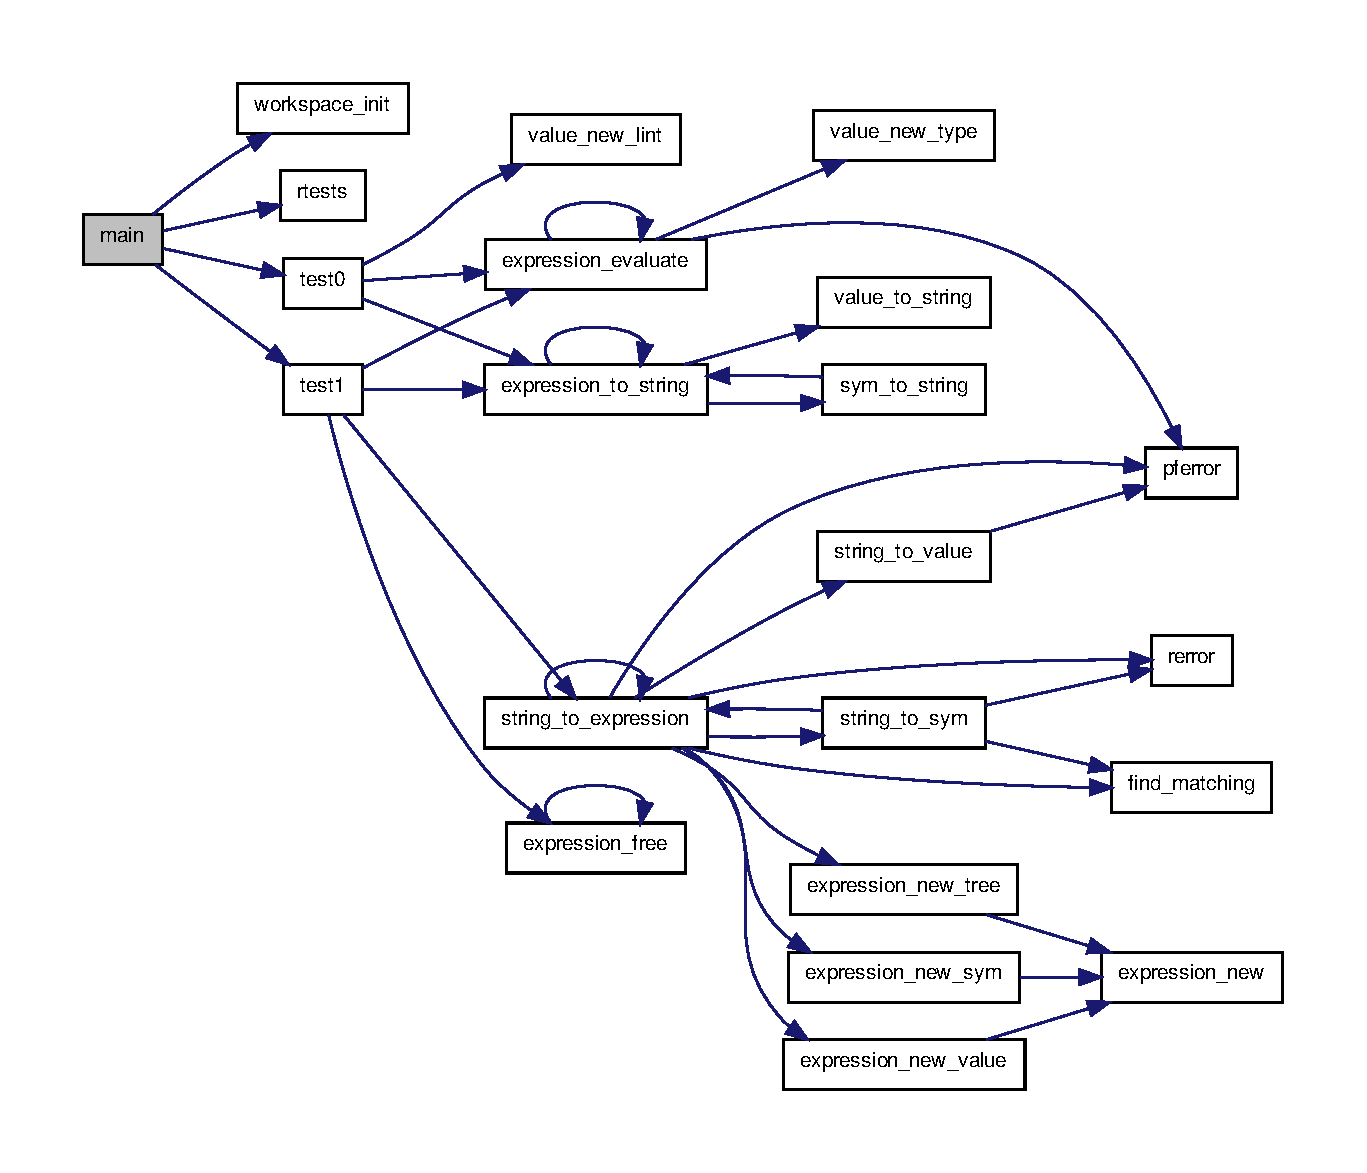
\includegraphics[width=350pt]{main_8c_a0ddf1224851353fc92bfbff6f499fa97_cgraph}
\end{center}
\end{figure}


\hypertarget{main_8c_ad7a5fe9ac7cb34a8455d013cc154283b}{\index{main.\+c@{main.\+c}!rtests@{rtests}}
\index{rtests@{rtests}!main.\+c@{main.\+c}}
\subsubsection[{rtests}]{\setlength{\rightskip}{0pt plus 5cm}void rtests (
\begin{DoxyParamCaption}
\item[{void}]{}
\end{DoxyParamCaption}
)}}\label{main_8c_ad7a5fe9ac7cb34a8455d013cc154283b}


Random Tests. 

Tests the atol() system function. Execute atol(). \hypertarget{main_8c_a2b5008f0c056e4e83b3ead2c95e50297}{\index{main.\+c@{main.\+c}!test0@{test0}}
\index{test0@{test0}!main.\+c@{main.\+c}}
\subsubsection[{test0}]{\setlength{\rightskip}{0pt plus 5cm}void test0 (
\begin{DoxyParamCaption}
\item[{void}]{}
\end{DoxyParamCaption}
)}}\label{main_8c_a2b5008f0c056e4e83b3ead2c95e50297}


Tests \hyperlink{expression__lite_8h_aca3bb6ea526afbf4f238a0877fe3e131}{expression\+\_\+to\+\_\+string} and then \hyperlink{expression__lite_8h_a70f3326a088855f6916f04baf27feed3}{expression\+\_\+evaluate} functions. 

It tests expression\+\_\+to\+\_\+string and expression\+\_\+evaluate on a manually created expression. The expression is ( (10 + 20) + 128 ) where e4 is the outer most root node and e3 is inner parent node of e0 and e1.

\begin{center}

\begin{DoxyImageNoCaption}
  \mbox{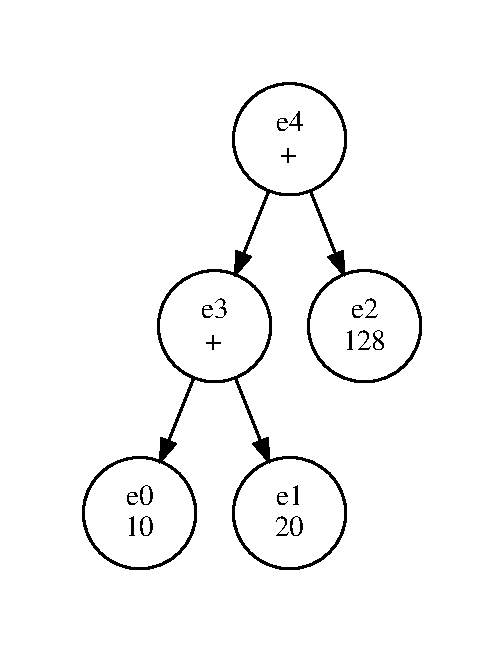
\includegraphics[width=\textwidth,height=\textheight/2,keepaspectratio=true]{dot_inline_dotgraph_1}}
\end{DoxyImageNoCaption}
\end{center}
 Call \hyperlink{types_8h_ab4456b47af2527b772ee8db5a367c66b}{value\+\_\+new\+\_\+lint} for e0 e1 and e2. 
\begin{DoxyCode}
puts(\textcolor{stringliteral}{"## Try value\_new\_lint()"});
e0.data.val = \hyperlink{types_8c_ab4456b47af2527b772ee8db5a367c66b}{value\_new\_lint}(10);
e1.data.val = \hyperlink{types_8c_ab4456b47af2527b772ee8db5a367c66b}{value\_new\_lint}(20);
e2.data.val = \hyperlink{types_8c_ab4456b47af2527b772ee8db5a367c66b}{value\_new\_lint}(128);
\end{DoxyCode}


Call \hyperlink{expression__lite_8h_aca3bb6ea526afbf4f238a0877fe3e131}{expression\+\_\+to\+\_\+string} on e4. 
\begin{DoxyCode}
puts(\textcolor{stringliteral}{"## Try expression\_to\_string()"});
\textcolor{comment}{// get string of root node e4}
\hyperlink{expression_8c_aca3bb6ea526afbf4f238a0877fe3e131}{expression\_to\_string}(buf, &e4);
puts(\textcolor{stringliteral}{"## Show resultant string"});
puts(\textcolor{stringliteral}{"Expect: "}\hyperlink{main_8c_a63b91eaa0a70d50671e305c4f1603b53}{EXPECT}(\textcolor{stringliteral}{"((10 + 20) + 128)"}));
printf(\textcolor{stringliteral}{"Expression String: "}\hyperlink{main_8c_ab6b4f9167f1d2de786d796d82f941454}{RESULT}(\textcolor{stringliteral}{"%s"})\textcolor{stringliteral}{"\(\backslash\)n"}, buf);
\end{DoxyCode}


Call \hyperlink{expression__lite_8h_a70f3326a088855f6916f04baf27feed3}{expression\+\_\+evaluate} on e4. 
\begin{DoxyCode}
puts(\textcolor{stringliteral}{"## Try expression\_evaluate()"});
result = \hyperlink{expression_8c_a70f3326a088855f6916f04baf27feed3}{expression\_evaluate}(&e4);
assert(result.type == \hyperlink{types_8h_a2763ddd86ab6e5f5f4c34c0561d4cd39a6910734ada9098e9409f17682d47c6bc}{VAL\_LINT});
puts(\textcolor{stringliteral}{"## Show resultant values"});
puts(\textcolor{stringliteral}{"Expect: "}\hyperlink{main_8c_a63b91eaa0a70d50671e305c4f1603b53}{EXPECT}(\textcolor{stringliteral}{"((10 + 20) + 128) = 158"}));
printf(\textcolor{stringliteral}{"Expression: "}\hyperlink{main_8c_ab6b4f9167f1d2de786d796d82f941454}{RESULT}(\textcolor{stringliteral}{"%s = %ld"})\textcolor{stringliteral}{"\(\backslash\)n"}, buf, result.data.lint);
\end{DoxyCode}
 

Here is the call graph for this function\+:\nopagebreak
\begin{figure}[H]
\begin{center}
\leavevmode
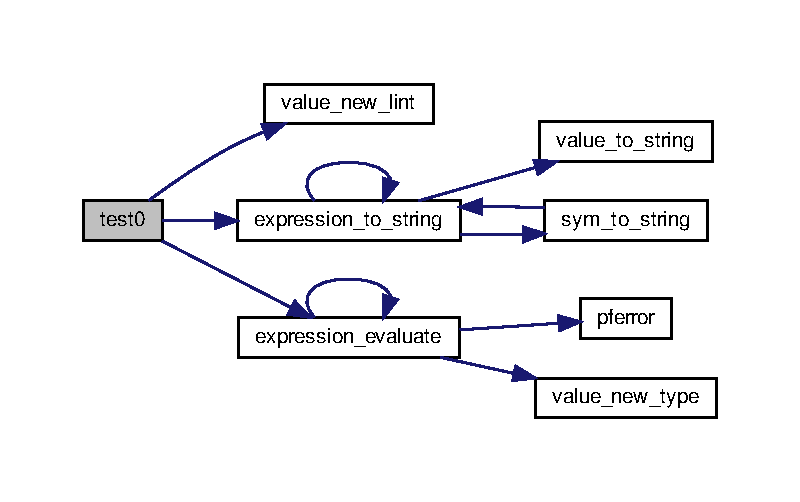
\includegraphics[width=350pt]{main_8c_a2b5008f0c056e4e83b3ead2c95e50297_cgraph}
\end{center}
\end{figure}


\hypertarget{main_8c_a299e410e6033d409446bd27bd4fb5b90}{\index{main.\+c@{main.\+c}!test1@{test1}}
\index{test1@{test1}!main.\+c@{main.\+c}}
\subsubsection[{test1}]{\setlength{\rightskip}{0pt plus 5cm}void test1 (
\begin{DoxyParamCaption}
\item[{char $\ast$}]{str}
\end{DoxyParamCaption}
)}}\label{main_8c_a299e410e6033d409446bd27bd4fb5b90}


Tests \hyperlink{expression__lite_8h_a63988c00ace0261c4896f132f5f86fda}{string\+\_\+to\+\_\+expression} on the string argument and then tests \hyperlink{expression__lite_8h_aca3bb6ea526afbf4f238a0877fe3e131}{expression\+\_\+to\+\_\+string} on it's output. 


\begin{DoxyParams}{Parameters}
{\em str} & The expression string to use. \\
\hline
\end{DoxyParams}
Call \hyperlink{expression__lite_8h_a63988c00ace0261c4896f132f5f86fda}{string\+\_\+to\+\_\+expression} on str 
\begin{DoxyCode}
e1 = \hyperlink{expression_8c_a63988c00ace0261c4896f132f5f86fda}{string\_to\_expression} (strlen(str), str);
\end{DoxyCode}


Call \hyperlink{expression__lite_8h_aca3bb6ea526afbf4f238a0877fe3e131}{expression\+\_\+to\+\_\+string} on result, e1 
\begin{DoxyCode}
\hyperlink{expression_8c_aca3bb6ea526afbf4f238a0877fe3e131}{expression\_to\_string} (buf,  e1);
\end{DoxyCode}
 

Here is the call graph for this function\+:\nopagebreak
\begin{figure}[H]
\begin{center}
\leavevmode
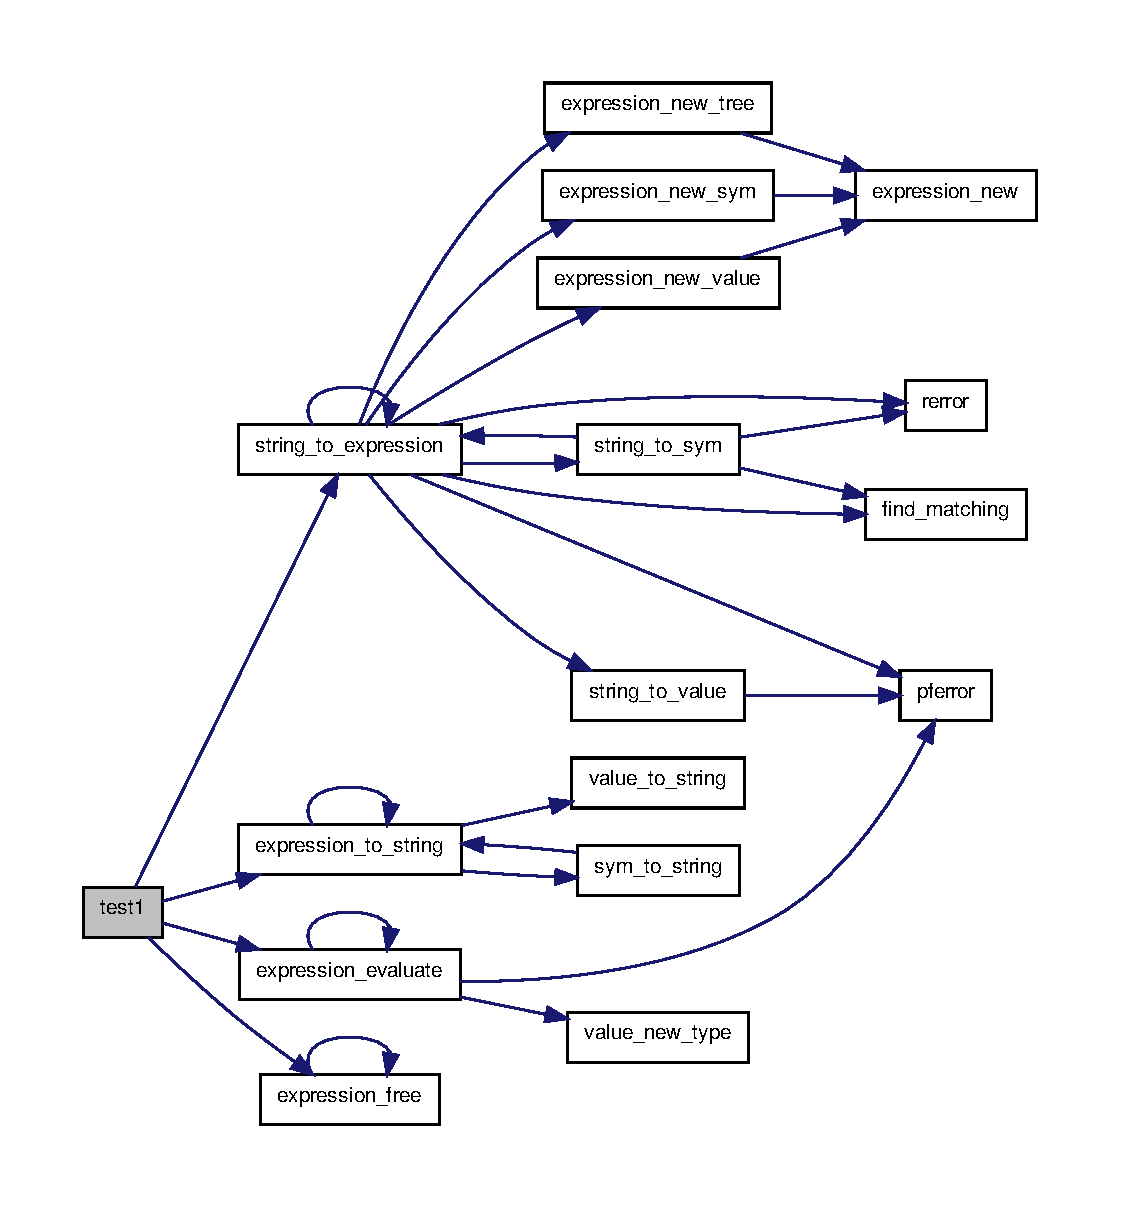
\includegraphics[width=350pt]{main_8c_a299e410e6033d409446bd27bd4fb5b90_cgraph}
\end{center}
\end{figure}



\hypertarget{README_8md}{}\section{R\+E\+A\+D\+M\+E.\+md File Reference}
\label{README_8md}\index{R\+E\+A\+D\+M\+E.\+md@{R\+E\+A\+D\+M\+E.\+md}}

\hypertarget{symbolic_8c}{\section{symbolic.\+c File Reference}
\label{symbolic_8c}\index{symbolic.\+c@{symbolic.\+c}}
}
{\ttfamily \#include $<$stdio.\+h$>$}\\*
{\ttfamily \#include $<$string.\+h$>$}\\*
{\ttfamily \#include \char`\"{}types.\+h\char`\"{}}\\*
{\ttfamily \#include \char`\"{}errors.\+h\char`\"{}}\\*
{\ttfamily \#include \char`\"{}symbolic.\+h\char`\"{}}\\*
Include dependency graph for symbolic.\+c\+:\nopagebreak
\begin{figure}[H]
\begin{center}
\leavevmode
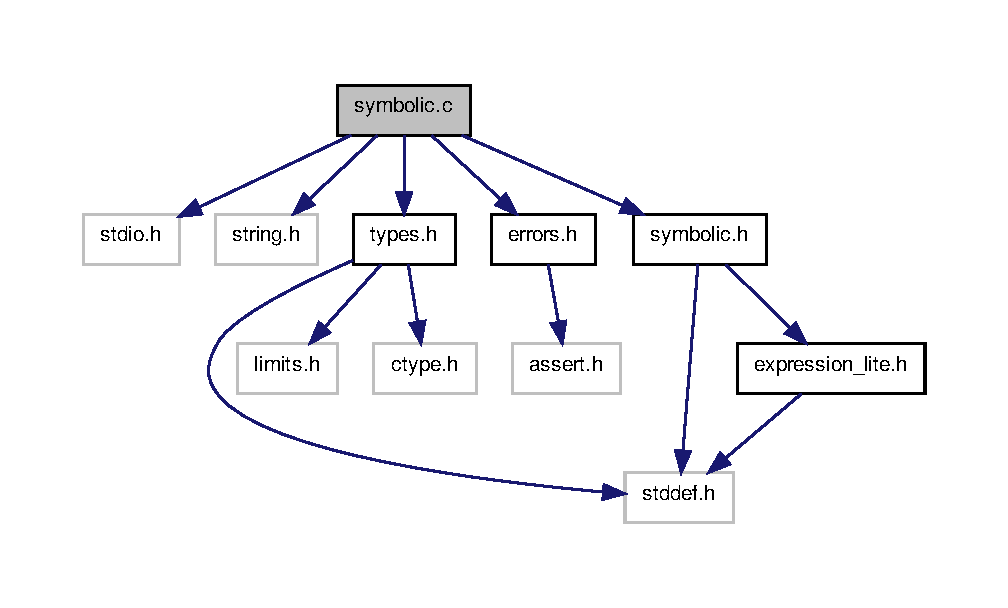
\includegraphics[width=350pt]{symbolic_8c__incl}
\end{center}
\end{figure}
\subsection*{Functions}
\begin{DoxyCompactItemize}
\item 
\hyperlink{symbolic_8h_a32ce0f63fa539078e25332dae6b7c77c}{sym\+\_\+t} \hyperlink{symbolic_8c_a51d47153d7323b2941308b506bd90578}{sym\+\_\+new\+\_\+name} (char $\ast$name)
\begin{DoxyCompactList}\small\item\em New symbolic object whose name is set to name. \end{DoxyCompactList}\item 
\hyperlink{symbolic_8h_a32ce0f63fa539078e25332dae6b7c77c}{sym\+\_\+t} \hyperlink{symbolic_8c_a78aa047f421c2d8ab5fab3c72d123d1b}{string\+\_\+to\+\_\+sym} (size\+\_\+t src\+\_\+str\+\_\+len, char const $\ast$src\+\_\+str)
\begin{DoxyCompactList}\small\item\em Create symbol from a string. \end{DoxyCompactList}\item 
void \hyperlink{symbolic_8c_a6a546d8b16eb1a91b309869b5d37cfc6}{sym\+\_\+to\+\_\+string} (char $\ast$dst\+\_\+str, \hyperlink{symbolic_8h_a32ce0f63fa539078e25332dae6b7c77c}{sym\+\_\+t} src\+\_\+sym)
\begin{DoxyCompactList}\small\item\em Generate a string from a sym\+\_\+t. \end{DoxyCompactList}\end{DoxyCompactItemize}


\subsection{Detailed Description}
\begin{DoxyDate}{Date}
May 3, 2014 
\end{DoxyDate}
\begin{DoxyAuthor}{Author}
Craig Hesling 
\end{DoxyAuthor}


\subsection{Function Documentation}
\hypertarget{symbolic_8c_a78aa047f421c2d8ab5fab3c72d123d1b}{\index{symbolic.\+c@{symbolic.\+c}!string\+\_\+to\+\_\+sym@{string\+\_\+to\+\_\+sym}}
\index{string\+\_\+to\+\_\+sym@{string\+\_\+to\+\_\+sym}!symbolic.\+c@{symbolic.\+c}}
\subsubsection[{string\+\_\+to\+\_\+sym}]{\setlength{\rightskip}{0pt plus 5cm}{\bf sym\+\_\+t} string\+\_\+to\+\_\+sym (
\begin{DoxyParamCaption}
\item[{size\+\_\+t}]{src\+\_\+str\+\_\+len, }
\item[{char const $\ast$}]{src\+\_\+str}
\end{DoxyParamCaption}
)}}\label{symbolic_8c_a78aa047f421c2d8ab5fab3c72d123d1b}


Create symbol from a string. 


\begin{DoxyParams}{Parameters}
{\em src\+\_\+str\+\_\+len} & The length of the actual buffer (not the number size). \\
\hline
{\em src\+\_\+str} & The source string. \\
\hline
\end{DoxyParams}
\begin{DoxyReturn}{Returns}
The symbol in the source string. 
\end{DoxyReturn}
\begin{DoxyNote}{Note}
Must have first char be digit 

Currently we only do Long Ints 
\end{DoxyNote}
$<$ Used to explore the presence of a symbol parameter 

Here is the call graph for this function\+:\nopagebreak
\begin{figure}[H]
\begin{center}
\leavevmode
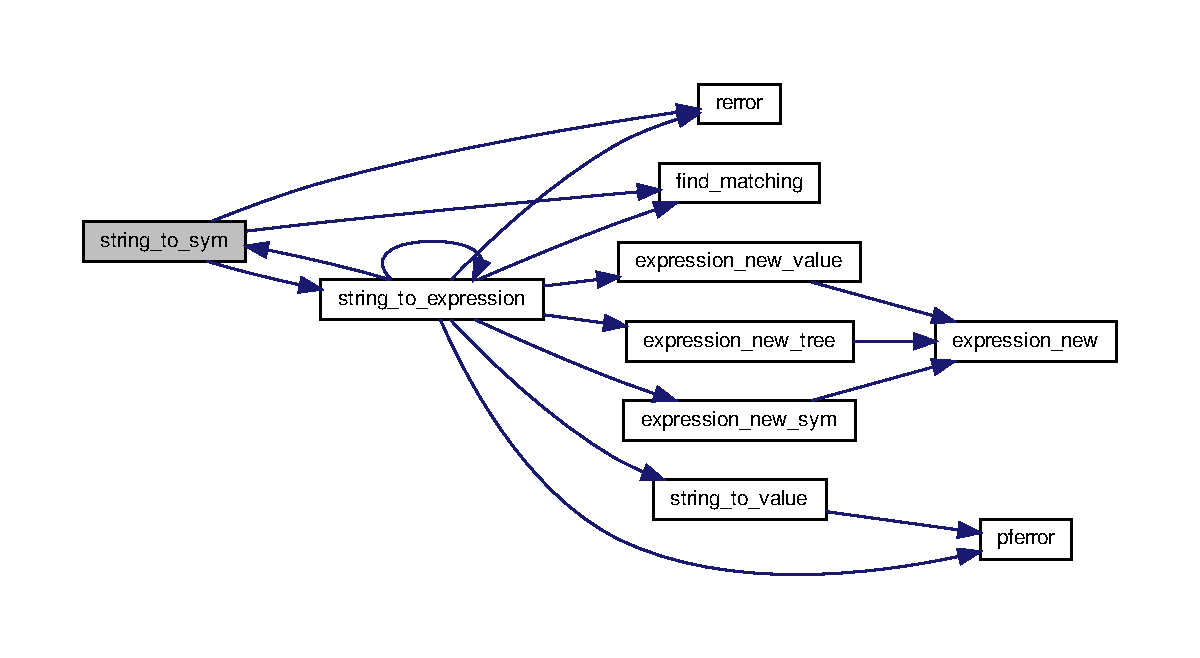
\includegraphics[width=350pt]{symbolic_8c_a78aa047f421c2d8ab5fab3c72d123d1b_cgraph}
\end{center}
\end{figure}


\hypertarget{symbolic_8c_a51d47153d7323b2941308b506bd90578}{\index{symbolic.\+c@{symbolic.\+c}!sym\+\_\+new\+\_\+name@{sym\+\_\+new\+\_\+name}}
\index{sym\+\_\+new\+\_\+name@{sym\+\_\+new\+\_\+name}!symbolic.\+c@{symbolic.\+c}}
\subsubsection[{sym\+\_\+new\+\_\+name}]{\setlength{\rightskip}{0pt plus 5cm}{\bf sym\+\_\+t} sym\+\_\+new\+\_\+name (
\begin{DoxyParamCaption}
\item[{char $\ast$}]{name}
\end{DoxyParamCaption}
)}}\label{symbolic_8c_a51d47153d7323b2941308b506bd90578}


New symbolic object whose name is set to name. 

\begin{DoxyRefDesc}{Todo}
\item[\hyperlink{todo__todo000005}{Todo}]Should probably check that the name contains valid chars (printable) \end{DoxyRefDesc}
\hypertarget{symbolic_8c_a6a546d8b16eb1a91b309869b5d37cfc6}{\index{symbolic.\+c@{symbolic.\+c}!sym\+\_\+to\+\_\+string@{sym\+\_\+to\+\_\+string}}
\index{sym\+\_\+to\+\_\+string@{sym\+\_\+to\+\_\+string}!symbolic.\+c@{symbolic.\+c}}
\subsubsection[{sym\+\_\+to\+\_\+string}]{\setlength{\rightskip}{0pt plus 5cm}void sym\+\_\+to\+\_\+string (
\begin{DoxyParamCaption}
\item[{char $\ast$}]{dst\+\_\+str, }
\item[{{\bf sym\+\_\+t}}]{src\+\_\+sym}
\end{DoxyParamCaption}
)}}\label{symbolic_8c_a6a546d8b16eb1a91b309869b5d37cfc6}


Generate a string from a sym\+\_\+t. 


\begin{DoxyParams}{Parameters}
{\em dst\+\_\+str} & String to write to. \\
\hline
{\em src\+\_\+sym} & Symbolic type to read from. \\
\hline
\end{DoxyParams}


Here is the call graph for this function\+:\nopagebreak
\begin{figure}[H]
\begin{center}
\leavevmode
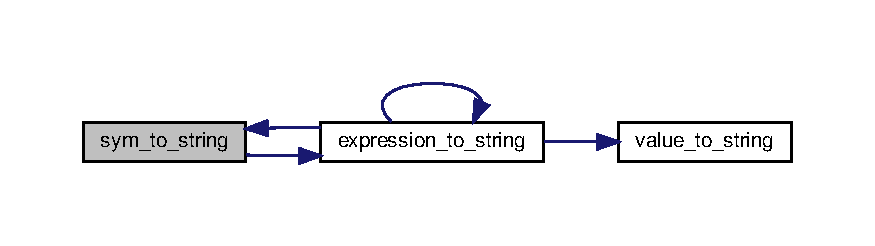
\includegraphics[width=350pt]{symbolic_8c_a6a546d8b16eb1a91b309869b5d37cfc6_cgraph}
\end{center}
\end{figure}



\hypertarget{symbolic_8h}{}\section{symbolic.\+h File Reference}
\label{symbolic_8h}\index{symbolic.\+h@{symbolic.\+h}}
{\ttfamily \#include $<$stddef.\+h$>$}\newline
{\ttfamily \#include \char`\"{}expression\+\_\+lite.\+h\char`\"{}}\newline
Include dependency graph for symbolic.\+h\+:
\nopagebreak
\begin{figure}[H]
\begin{center}
\leavevmode
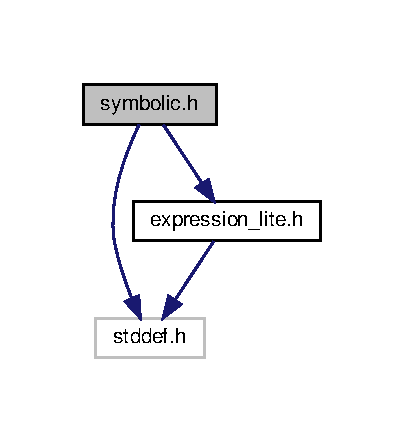
\includegraphics[width=194pt]{symbolic_8h__incl}
\end{center}
\end{figure}
\subsection*{Data Structures}
\begin{DoxyCompactItemize}
\item 
struct \hyperlink{structsym}{sym}
\begin{DoxyCompactList}\small\item\em A named symbol type. \end{DoxyCompactList}\end{DoxyCompactItemize}
\subsection*{Macros}
\begin{DoxyCompactItemize}
\item 
\#define \hyperlink{symbolic_8h_aeb7545cf4c9c6df72954b9409a00a885}{S\+Y\+M\+B\+O\+L\+I\+C\+\_\+\+N\+A\+M\+E\+\_\+\+S\+I\+ZE}~10
\item 
\#define \hyperlink{symbolic_8h_a171adf6d50315c5e3af7aaaef3bd90ce}{S\+Y\+M\+B\+O\+L\+I\+C\+\_\+\+P\+\_\+\+S\+T\+R\+\_\+\+S\+I\+ZE}~16
\end{DoxyCompactItemize}
\subsection*{Typedefs}
\begin{DoxyCompactItemize}
\item 
typedef struct \hyperlink{structsym}{sym} \hyperlink{symbolic_8h_a32ce0f63fa539078e25332dae6b7c77c}{sym\+\_\+t}
\end{DoxyCompactItemize}
\subsection*{Functions}
\begin{DoxyCompactItemize}
\item 
\hyperlink{symbolic_8h_a32ce0f63fa539078e25332dae6b7c77c}{sym\+\_\+t} \hyperlink{symbolic_8h_a51d47153d7323b2941308b506bd90578}{sym\+\_\+new\+\_\+name} (char $\ast$name)
\begin{DoxyCompactList}\small\item\em New symbolic object whose name is set to name. \end{DoxyCompactList}\item 
\hyperlink{symbolic_8h_a32ce0f63fa539078e25332dae6b7c77c}{sym\+\_\+t} \hyperlink{symbolic_8h_a78aa047f421c2d8ab5fab3c72d123d1b}{string\+\_\+to\+\_\+sym} (size\+\_\+t src\+\_\+str\+\_\+len, char const $\ast$src\+\_\+str)
\begin{DoxyCompactList}\small\item\em Create symbol from a string. \end{DoxyCompactList}\item 
void \hyperlink{symbolic_8h_a6a546d8b16eb1a91b309869b5d37cfc6}{sym\+\_\+to\+\_\+string} (char $\ast$dst\+\_\+str, \hyperlink{symbolic_8h_a32ce0f63fa539078e25332dae6b7c77c}{sym\+\_\+t} src\+\_\+sym)
\begin{DoxyCompactList}\small\item\em Generate a string from a sym\+\_\+t. \end{DoxyCompactList}\end{DoxyCompactItemize}


\subsection{Detailed Description}
\begin{DoxyDate}{Date}
May 3, 2014 
\end{DoxyDate}
\begin{DoxyAuthor}{Author}
Craig Hesling
\end{DoxyAuthor}
A light structure that is mostly public access.

The point of the sym structure is to create a string based reference to an object without being directly connected to the object. This allows for 

\subsection{Macro Definition Documentation}
\mbox{\Hypertarget{symbolic_8h_aeb7545cf4c9c6df72954b9409a00a885}\label{symbolic_8h_aeb7545cf4c9c6df72954b9409a00a885}} 
\index{symbolic.\+h@{symbolic.\+h}!S\+Y\+M\+B\+O\+L\+I\+C\+\_\+\+N\+A\+M\+E\+\_\+\+S\+I\+ZE@{S\+Y\+M\+B\+O\+L\+I\+C\+\_\+\+N\+A\+M\+E\+\_\+\+S\+I\+ZE}}
\index{S\+Y\+M\+B\+O\+L\+I\+C\+\_\+\+N\+A\+M\+E\+\_\+\+S\+I\+ZE@{S\+Y\+M\+B\+O\+L\+I\+C\+\_\+\+N\+A\+M\+E\+\_\+\+S\+I\+ZE}!symbolic.\+h@{symbolic.\+h}}
\subsubsection{\texorpdfstring{S\+Y\+M\+B\+O\+L\+I\+C\+\_\+\+N\+A\+M\+E\+\_\+\+S\+I\+ZE}{SYMBOLIC\_NAME\_SIZE}}
{\footnotesize\ttfamily \#define S\+Y\+M\+B\+O\+L\+I\+C\+\_\+\+N\+A\+M\+E\+\_\+\+S\+I\+ZE~10}

\mbox{\Hypertarget{symbolic_8h_a171adf6d50315c5e3af7aaaef3bd90ce}\label{symbolic_8h_a171adf6d50315c5e3af7aaaef3bd90ce}} 
\index{symbolic.\+h@{symbolic.\+h}!S\+Y\+M\+B\+O\+L\+I\+C\+\_\+\+P\+\_\+\+S\+T\+R\+\_\+\+S\+I\+ZE@{S\+Y\+M\+B\+O\+L\+I\+C\+\_\+\+P\+\_\+\+S\+T\+R\+\_\+\+S\+I\+ZE}}
\index{S\+Y\+M\+B\+O\+L\+I\+C\+\_\+\+P\+\_\+\+S\+T\+R\+\_\+\+S\+I\+ZE@{S\+Y\+M\+B\+O\+L\+I\+C\+\_\+\+P\+\_\+\+S\+T\+R\+\_\+\+S\+I\+ZE}!symbolic.\+h@{symbolic.\+h}}
\subsubsection{\texorpdfstring{S\+Y\+M\+B\+O\+L\+I\+C\+\_\+\+P\+\_\+\+S\+T\+R\+\_\+\+S\+I\+ZE}{SYMBOLIC\_P\_STR\_SIZE}}
{\footnotesize\ttfamily \#define S\+Y\+M\+B\+O\+L\+I\+C\+\_\+\+P\+\_\+\+S\+T\+R\+\_\+\+S\+I\+ZE~16}



\subsection{Typedef Documentation}
\mbox{\Hypertarget{symbolic_8h_a32ce0f63fa539078e25332dae6b7c77c}\label{symbolic_8h_a32ce0f63fa539078e25332dae6b7c77c}} 
\index{symbolic.\+h@{symbolic.\+h}!sym\+\_\+t@{sym\+\_\+t}}
\index{sym\+\_\+t@{sym\+\_\+t}!symbolic.\+h@{symbolic.\+h}}
\subsubsection{\texorpdfstring{sym\+\_\+t}{sym\_t}}
{\footnotesize\ttfamily typedef struct \hyperlink{structsym}{sym} \hyperlink{symbolic_8h_a32ce0f63fa539078e25332dae6b7c77c}{sym\+\_\+t}}



\subsection{Function Documentation}
\mbox{\Hypertarget{symbolic_8h_a78aa047f421c2d8ab5fab3c72d123d1b}\label{symbolic_8h_a78aa047f421c2d8ab5fab3c72d123d1b}} 
\index{symbolic.\+h@{symbolic.\+h}!string\+\_\+to\+\_\+sym@{string\+\_\+to\+\_\+sym}}
\index{string\+\_\+to\+\_\+sym@{string\+\_\+to\+\_\+sym}!symbolic.\+h@{symbolic.\+h}}
\subsubsection{\texorpdfstring{string\+\_\+to\+\_\+sym()}{string\_to\_sym()}}
{\footnotesize\ttfamily \hyperlink{symbolic_8h_a32ce0f63fa539078e25332dae6b7c77c}{sym\+\_\+t} string\+\_\+to\+\_\+sym (\begin{DoxyParamCaption}\item[{size\+\_\+t}]{src\+\_\+str\+\_\+len,  }\item[{char const $\ast$}]{src\+\_\+str }\end{DoxyParamCaption})}



Create symbol from a string. 


\begin{DoxyParams}{Parameters}
{\em src\+\_\+str\+\_\+len} & The length of the actual buffer (not the number size). \\
\hline
{\em src\+\_\+str} & The source string. \\
\hline
\end{DoxyParams}
\begin{DoxyReturn}{Returns}
The symbol in the source string. 
\end{DoxyReturn}
\begin{DoxyNote}{Note}
Must have first char be digit 

Currently we only do Long Ints 
\end{DoxyNote}
$<$ Used to explore the presence of a symbol parameter Here is the call graph for this function\+:
\nopagebreak
\begin{figure}[H]
\begin{center}
\leavevmode
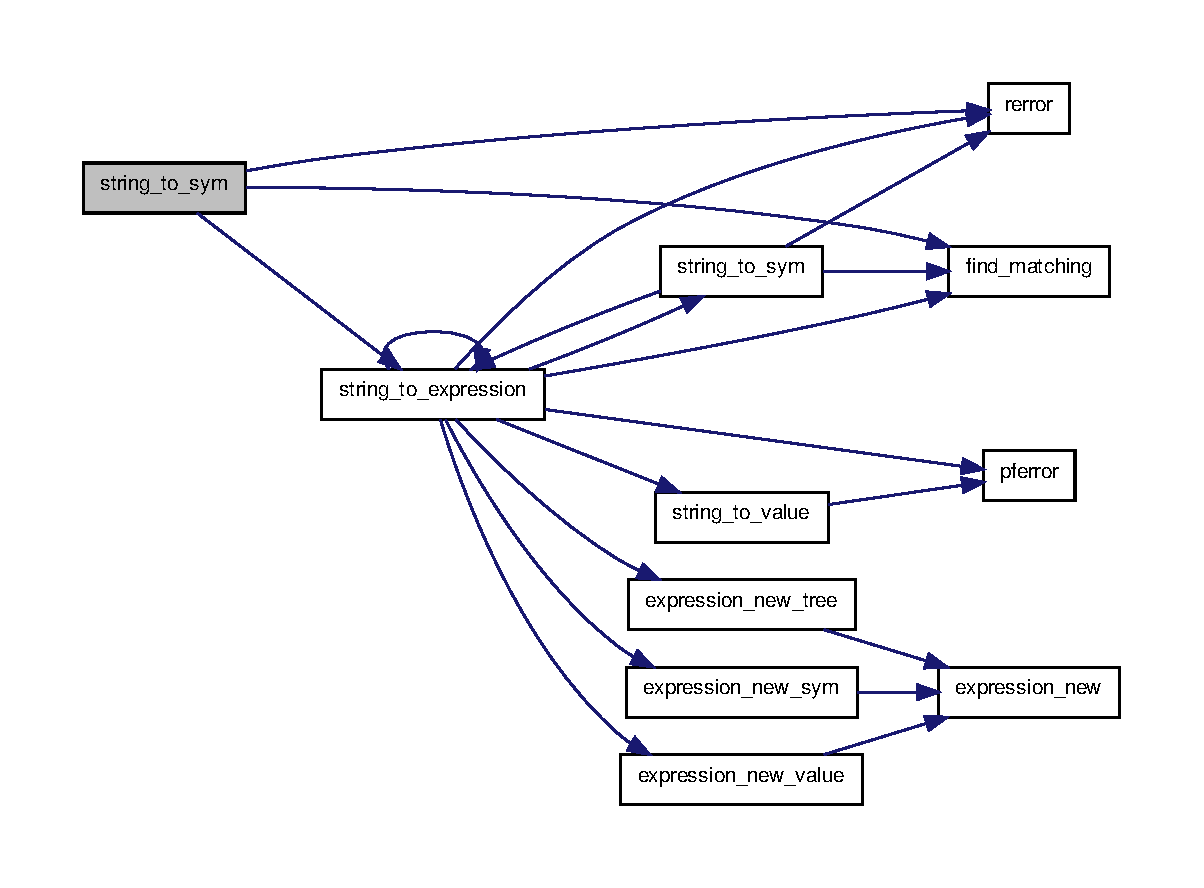
\includegraphics[width=350pt]{symbolic_8h_a78aa047f421c2d8ab5fab3c72d123d1b_cgraph}
\end{center}
\end{figure}
\mbox{\Hypertarget{symbolic_8h_a51d47153d7323b2941308b506bd90578}\label{symbolic_8h_a51d47153d7323b2941308b506bd90578}} 
\index{symbolic.\+h@{symbolic.\+h}!sym\+\_\+new\+\_\+name@{sym\+\_\+new\+\_\+name}}
\index{sym\+\_\+new\+\_\+name@{sym\+\_\+new\+\_\+name}!symbolic.\+h@{symbolic.\+h}}
\subsubsection{\texorpdfstring{sym\+\_\+new\+\_\+name()}{sym\_new\_name()}}
{\footnotesize\ttfamily \hyperlink{symbolic_8h_a32ce0f63fa539078e25332dae6b7c77c}{sym\+\_\+t} sym\+\_\+new\+\_\+name (\begin{DoxyParamCaption}\item[{char $\ast$}]{name }\end{DoxyParamCaption})}



New symbolic object whose name is set to name. 

\begin{DoxyRefDesc}{Todo}
\item[\hyperlink{todo__todo000005}{Todo}]Should probably check that the name contains valid chars (printable) \end{DoxyRefDesc}
\mbox{\Hypertarget{symbolic_8h_a6a546d8b16eb1a91b309869b5d37cfc6}\label{symbolic_8h_a6a546d8b16eb1a91b309869b5d37cfc6}} 
\index{symbolic.\+h@{symbolic.\+h}!sym\+\_\+to\+\_\+string@{sym\+\_\+to\+\_\+string}}
\index{sym\+\_\+to\+\_\+string@{sym\+\_\+to\+\_\+string}!symbolic.\+h@{symbolic.\+h}}
\subsubsection{\texorpdfstring{sym\+\_\+to\+\_\+string()}{sym\_to\_string()}}
{\footnotesize\ttfamily void sym\+\_\+to\+\_\+string (\begin{DoxyParamCaption}\item[{char $\ast$}]{dst\+\_\+str,  }\item[{\hyperlink{symbolic_8h_a32ce0f63fa539078e25332dae6b7c77c}{sym\+\_\+t}}]{src\+\_\+sym }\end{DoxyParamCaption})}



Generate a string from a sym\+\_\+t. 


\begin{DoxyParams}{Parameters}
{\em dst\+\_\+str} & String to write to. \\
\hline
{\em src\+\_\+sym} & Symbolic type to read from. \\
\hline
\end{DoxyParams}
Here is the call graph for this function\+:
\nopagebreak
\begin{figure}[H]
\begin{center}
\leavevmode
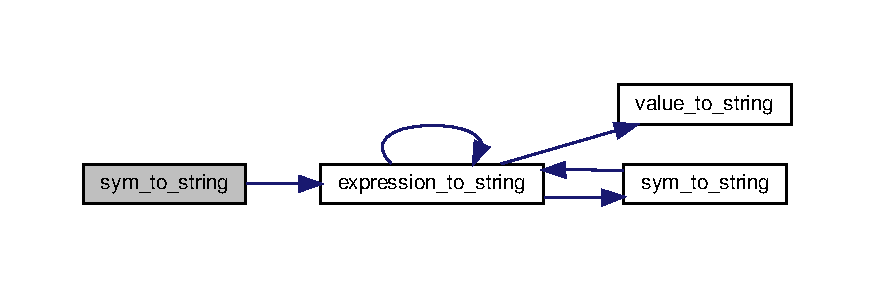
\includegraphics[width=350pt]{symbolic_8h_a6a546d8b16eb1a91b309869b5d37cfc6_cgraph}
\end{center}
\end{figure}

\hypertarget{types_8c}{}\section{types.\+c File Reference}
\label{types_8c}\index{types.\+c@{types.\+c}}
{\ttfamily \#include $<$stdio.\+h$>$}\newline
{\ttfamily \#include $<$stddef.\+h$>$}\newline
{\ttfamily \#include $<$stdlib.\+h$>$}\newline
{\ttfamily \#include \char`\"{}errors.\+h\char`\"{}}\newline
{\ttfamily \#include \char`\"{}expression.\+h\char`\"{}}\newline
{\ttfamily \#include \char`\"{}types.\+h\char`\"{}}\newline
Include dependency graph for types.\+c\+:
\nopagebreak
\begin{figure}[H]
\begin{center}
\leavevmode
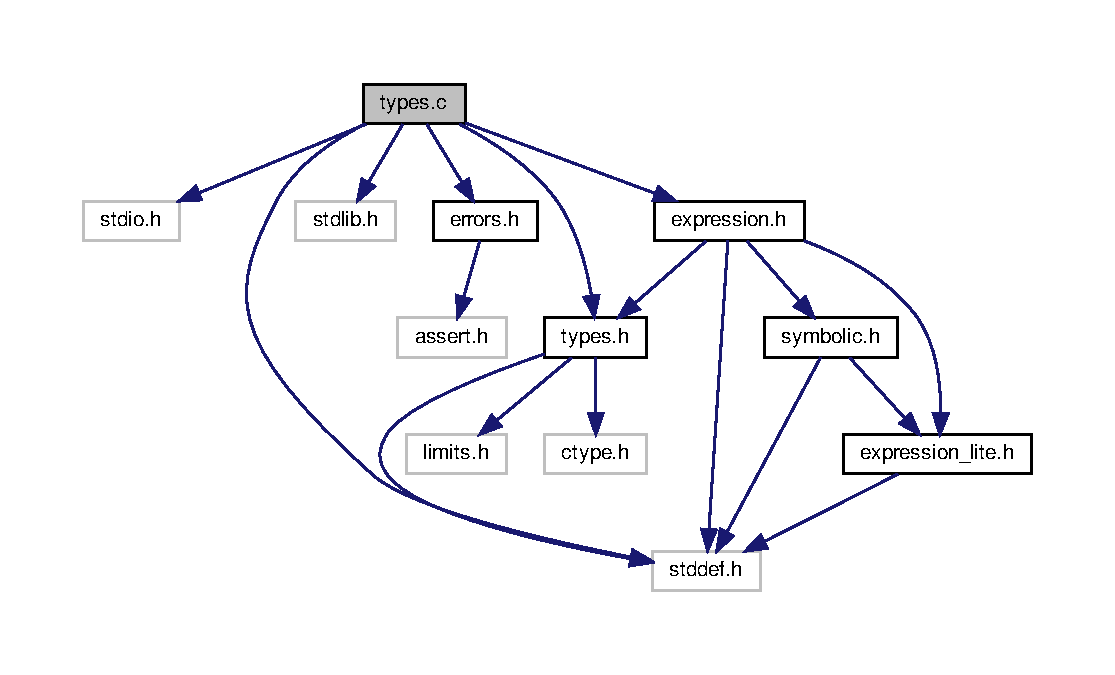
\includegraphics[width=350pt]{types_8c__incl}
\end{center}
\end{figure}
\subsection*{Functions}
\begin{DoxyCompactItemize}
\item 
\hyperlink{types_8h_ae4d4f561b975159d5852cb2c30bf20ef}{value\+\_\+t} \hyperlink{types_8c_a82b79a7bbb2da51fd09d5f5c90c5105a}{value\+\_\+new\+\_\+type} (enum \hyperlink{types_8h_a2763ddd86ab6e5f5f4c34c0561d4cd39}{value\+\_\+types} type)
\item 
\hyperlink{types_8h_ae4d4f561b975159d5852cb2c30bf20ef}{value\+\_\+t} \hyperlink{types_8c_ab4456b47af2527b772ee8db5a367c66b}{value\+\_\+new\+\_\+lint} (\hyperlink{types_8h_a5b2030ae244cd6621f11f4bf6d181dbf}{sys\+\_\+int\+\_\+long} lint)
\item 
\hyperlink{types_8h_ae4d4f561b975159d5852cb2c30bf20ef}{value\+\_\+t} \hyperlink{types_8c_a9c194ae881900b4376e761e2294117f9}{string\+\_\+to\+\_\+value} (size\+\_\+t src\+\_\+str\+\_\+len, char const $\ast$src\+\_\+str)
\begin{DoxyCompactList}\small\item\em Create value from a string. \end{DoxyCompactList}\item 
void \hyperlink{types_8c_a4560a9f9bfc3ee07f105b16cc4230964}{value\+\_\+to\+\_\+string} (char $\ast$dst\+\_\+str, \hyperlink{types_8h_ae4d4f561b975159d5852cb2c30bf20ef}{value\+\_\+t} src\+\_\+val)
\item 
\hyperlink{types_8h_adf276b495f7366f87ee85dc7df2fe32e}{pindex\+\_\+t} \hyperlink{types_8c_a57807e65ff8a4886f850f98d347e44fc}{find\+\_\+matching} (size\+\_\+t str\+\_\+len, const char $\ast$str, \hyperlink{types_8h_adf276b495f7366f87ee85dc7df2fe32e}{pindex\+\_\+t} start)
\begin{DoxyCompactList}\small\item\em Find the index of the matching closing paren in a string. \end{DoxyCompactList}\end{DoxyCompactItemize}


\subsection{Detailed Description}
\begin{DoxyDate}{Date}
Apr 23, 2014 
\end{DoxyDate}
\begin{DoxyAuthor}{Author}
Craig Hesling
\end{DoxyAuthor}
Contains standard types, macros, and functions used throughout the library. Most notably, this is the home of the \hyperlink{types_8h_ae4d4f561b975159d5852cb2c30bf20ef}{value\+\_\+t}. 

\subsection{Function Documentation}
\mbox{\Hypertarget{types_8c_a57807e65ff8a4886f850f98d347e44fc}\label{types_8c_a57807e65ff8a4886f850f98d347e44fc}} 
\index{types.\+c@{types.\+c}!find\+\_\+matching@{find\+\_\+matching}}
\index{find\+\_\+matching@{find\+\_\+matching}!types.\+c@{types.\+c}}
\subsubsection{\texorpdfstring{find\+\_\+matching()}{find\_matching()}}
{\footnotesize\ttfamily \hyperlink{types_8h_adf276b495f7366f87ee85dc7df2fe32e}{pindex\+\_\+t} find\+\_\+matching (\begin{DoxyParamCaption}\item[{size\+\_\+t}]{str\+\_\+len,  }\item[{const char $\ast$}]{str,  }\item[{\hyperlink{types_8h_adf276b495f7366f87ee85dc7df2fe32e}{pindex\+\_\+t}}]{start }\end{DoxyParamCaption})}



Find the index of the matching closing paren in a string. 


\begin{DoxyParams}{Parameters}
{\em str\+\_\+len} & Overall string length. \\
\hline
{\em str} & String to search in. \\
\hline
{\em start} & Index of the open paren to match. \\
\hline
\end{DoxyParams}
\begin{DoxyReturn}{Returns}
The index of the matching paren or P\+I\+N\+D\+E\+X\+\_\+\+B\+AD if no match was found. 
\end{DoxyReturn}
\begin{DoxyNote}{Note}
Assumes start is the index of the open paren to match and then moves forward. 
\end{DoxyNote}
\mbox{\Hypertarget{types_8c_a9c194ae881900b4376e761e2294117f9}\label{types_8c_a9c194ae881900b4376e761e2294117f9}} 
\index{types.\+c@{types.\+c}!string\+\_\+to\+\_\+value@{string\+\_\+to\+\_\+value}}
\index{string\+\_\+to\+\_\+value@{string\+\_\+to\+\_\+value}!types.\+c@{types.\+c}}
\subsubsection{\texorpdfstring{string\+\_\+to\+\_\+value()}{string\_to\_value()}}
{\footnotesize\ttfamily \hyperlink{types_8h_ae4d4f561b975159d5852cb2c30bf20ef}{value\+\_\+t} string\+\_\+to\+\_\+value (\begin{DoxyParamCaption}\item[{size\+\_\+t}]{src\+\_\+str\+\_\+len,  }\item[{char const $\ast$}]{src\+\_\+str }\end{DoxyParamCaption})}



Create value from a string. 


\begin{DoxyParams}{Parameters}
{\em src\+\_\+str\+\_\+len} & The length of the actual buffer (not the number size). \\
\hline
{\em src\+\_\+str} & The source string. \\
\hline
\end{DoxyParams}
\begin{DoxyReturn}{Returns}
The value in the source string. 
\end{DoxyReturn}
\begin{DoxyNote}{Note}
Must have first char be digit 

Currently we only do Long Ints 
\end{DoxyNote}
$<$ \begin{DoxyNote}{Note}
Here we assume it is a Long Int
\end{DoxyNote}
$<$ \begin{DoxyWarning}{Warning}
Uses system atol() function at index 0 on the bare string given 
\end{DoxyWarning}
Here is the call graph for this function\+:
\nopagebreak
\begin{figure}[H]
\begin{center}
\leavevmode
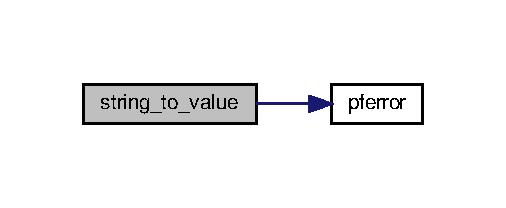
\includegraphics[width=243pt]{types_8c_a9c194ae881900b4376e761e2294117f9_cgraph}
\end{center}
\end{figure}
\mbox{\Hypertarget{types_8c_ab4456b47af2527b772ee8db5a367c66b}\label{types_8c_ab4456b47af2527b772ee8db5a367c66b}} 
\index{types.\+c@{types.\+c}!value\+\_\+new\+\_\+lint@{value\+\_\+new\+\_\+lint}}
\index{value\+\_\+new\+\_\+lint@{value\+\_\+new\+\_\+lint}!types.\+c@{types.\+c}}
\subsubsection{\texorpdfstring{value\+\_\+new\+\_\+lint()}{value\_new\_lint()}}
{\footnotesize\ttfamily \hyperlink{types_8h_ae4d4f561b975159d5852cb2c30bf20ef}{value\+\_\+t} value\+\_\+new\+\_\+lint (\begin{DoxyParamCaption}\item[{\hyperlink{types_8h_a5b2030ae244cd6621f11f4bf6d181dbf}{sys\+\_\+int\+\_\+long}}]{lint }\end{DoxyParamCaption})}

\mbox{\Hypertarget{types_8c_a82b79a7bbb2da51fd09d5f5c90c5105a}\label{types_8c_a82b79a7bbb2da51fd09d5f5c90c5105a}} 
\index{types.\+c@{types.\+c}!value\+\_\+new\+\_\+type@{value\+\_\+new\+\_\+type}}
\index{value\+\_\+new\+\_\+type@{value\+\_\+new\+\_\+type}!types.\+c@{types.\+c}}
\subsubsection{\texorpdfstring{value\+\_\+new\+\_\+type()}{value\_new\_type()}}
{\footnotesize\ttfamily \hyperlink{types_8h_ae4d4f561b975159d5852cb2c30bf20ef}{value\+\_\+t} value\+\_\+new\+\_\+type (\begin{DoxyParamCaption}\item[{enum \hyperlink{types_8h_a2763ddd86ab6e5f5f4c34c0561d4cd39}{value\+\_\+types}}]{type }\end{DoxyParamCaption})}

\mbox{\Hypertarget{types_8c_a4560a9f9bfc3ee07f105b16cc4230964}\label{types_8c_a4560a9f9bfc3ee07f105b16cc4230964}} 
\index{types.\+c@{types.\+c}!value\+\_\+to\+\_\+string@{value\+\_\+to\+\_\+string}}
\index{value\+\_\+to\+\_\+string@{value\+\_\+to\+\_\+string}!types.\+c@{types.\+c}}
\subsubsection{\texorpdfstring{value\+\_\+to\+\_\+string()}{value\_to\_string()}}
{\footnotesize\ttfamily void value\+\_\+to\+\_\+string (\begin{DoxyParamCaption}\item[{char $\ast$}]{dst\+\_\+str,  }\item[{\hyperlink{types_8h_ae4d4f561b975159d5852cb2c30bf20ef}{value\+\_\+t}}]{src\+\_\+val }\end{DoxyParamCaption})}

$<$ \begin{DoxyWarning}{Warning}
Unknown types of \hyperlink{types_8h_ae4d4f561b975159d5852cb2c30bf20ef}{value\+\_\+t} will just assert(false) here. 
\end{DoxyWarning}

\hypertarget{types_8h}{}\section{types.\+h File Reference}
\label{types_8h}\index{types.\+h@{types.\+h}}
{\ttfamily \#include $<$stddef.\+h$>$}\newline
{\ttfamily \#include $<$limits.\+h$>$}\newline
{\ttfamily \#include $<$ctype.\+h$>$}\newline
Include dependency graph for types.\+h\+:
\nopagebreak
\begin{figure}[H]
\begin{center}
\leavevmode
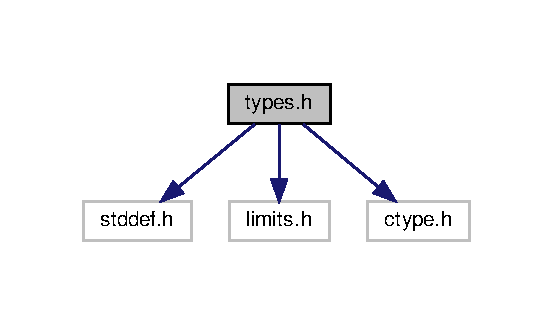
\includegraphics[width=266pt]{types_8h__incl}
\end{center}
\end{figure}
\subsection*{Data Structures}
\begin{DoxyCompactItemize}
\item 
union \hyperlink{unionvalue__data}{value\+\_\+data}
\begin{DoxyCompactList}\small\item\em value data container provider \end{DoxyCompactList}\item 
struct \hyperlink{structvalue}{value}
\begin{DoxyCompactList}\small\item\em Represents a numeric value or an error. \end{DoxyCompactList}\end{DoxyCompactItemize}
\subsection*{Macros}
\begin{DoxyCompactItemize}
\item 
\#define \hyperlink{types_8h_aceabf7297cb7a506a8d33c13f84ccdbd}{S\+Y\+S\+\_\+\+I\+N\+T\+\_\+\+L\+O\+N\+G\+\_\+\+T\+\_\+\+M\+IN}~L\+O\+N\+G\+\_\+\+M\+IN
\item 
\#define \hyperlink{types_8h_adee5b8951d2f6e25c90ae1d56a7950ec}{S\+Y\+S\+\_\+\+I\+N\+T\+\_\+\+L\+O\+N\+G\+\_\+\+T\+\_\+\+M\+AX}~L\+O\+N\+G\+\_\+\+M\+AX
\item 
\#define \hyperlink{types_8h_a1756477a6ac09ecf9676909a6a223430}{S\+Y\+S\+\_\+\+I\+N\+T\+\_\+\+L\+O\+N\+G\+\_\+\+T\+\_\+\+S\+T\+R\+\_\+\+S\+I\+ZE}~11
\begin{DoxyCompactList}\small\item\em The length in chars for a long int string. 4 byte long -\/ $ {\tt ceiling} \left( {\tt log10}(2^{4 \times 8 - 1}) \right) + 1$. \end{DoxyCompactList}\item 
\#define \hyperlink{types_8h_acfa3af56d5e0045c1d7a5682fd1d2853}{S\+I\+Z\+E\+\_\+\+T\+\_\+\+M\+AX}~( $\sim$( (size\+\_\+t) (0) ) )
\item 
\#define \hyperlink{types_8h_a8626f0b5f394221abc252d89bc034b23}{P\+I\+N\+D\+E\+X\+\_\+\+M\+AX}~\hyperlink{types_8h_acfa3af56d5e0045c1d7a5682fd1d2853}{S\+I\+Z\+E\+\_\+\+T\+\_\+\+M\+AX}
\begin{DoxyCompactList}\small\item\em The max value of pindex\+\_\+t. \end{DoxyCompactList}\item 
\#define \hyperlink{types_8h_ae48c70e63c613f1d1ce9b5b3753476ef}{P\+I\+N\+D\+E\+X\+\_\+\+B\+AD}~\hyperlink{types_8h_a8626f0b5f394221abc252d89bc034b23}{P\+I\+N\+D\+E\+X\+\_\+\+M\+AX}
\begin{DoxyCompactList}\small\item\em Special value of pindex\+\_\+t that signals a bad value. \end{DoxyCompactList}\item 
\#define \hyperlink{types_8h_a8e0cab4dcc3ef592793ac045edcd6344}{I\+S\+\_\+\+W\+H\+I\+T\+E\+S\+P\+A\+CE}(c)~( ((c) == \textquotesingle{} \textquotesingle{}) $\vert$$\vert$ ((c) == \textquotesingle{}\textbackslash{}t\textquotesingle{}) )
\item 
\#define \hyperlink{types_8h_a307c9de47db5ab41e0731cfd21c51e1d}{I\+S\+\_\+\+D\+I\+G\+IT}(c)~( ( \textquotesingle{}0\textquotesingle{} $<$= (c) ) \&\& ( (c) $<$= \textquotesingle{}9\textquotesingle{}) )
\item 
\#define \hyperlink{types_8h_abce481ac236ab589430f904c74ae2eba}{I\+S\+\_\+\+A\+L\+P\+HA}(c)~isalpha(c)
\item 
\#define \hyperlink{types_8h_a28e9f96038c5dd3ca26e8b5972ec16fc}{I\+S\+\_\+\+A\+L\+N\+UM}(c)~isalnum(c)
\end{DoxyCompactItemize}
\subsection*{Typedefs}
\begin{DoxyCompactItemize}
\item 
typedef int long \hyperlink{types_8h_a5b2030ae244cd6621f11f4bf6d181dbf}{sys\+\_\+int\+\_\+long}
\item 
typedef size\+\_\+t \hyperlink{types_8h_adf276b495f7366f87ee85dc7df2fe32e}{pindex\+\_\+t}
\begin{DoxyCompactList}\small\item\em Type for an index into an expression string during parsing. \end{DoxyCompactList}\item 
typedef size\+\_\+t \hyperlink{types_8h_adad1de15de2afe9201bfabbccf1e505e}{pcount\+\_\+t}
\begin{DoxyCompactList}\small\item\em Type for an item count during parsing. \end{DoxyCompactList}\item 
typedef struct \hyperlink{structvalue}{value} \hyperlink{types_8h_ae4d4f561b975159d5852cb2c30bf20ef}{value\+\_\+t}
\end{DoxyCompactItemize}
\subsection*{Enumerations}
\begin{DoxyCompactItemize}
\item 
enum \hyperlink{types_8h_a2763ddd86ab6e5f5f4c34c0561d4cd39}{value\+\_\+types} \{ \hyperlink{types_8h_a2763ddd86ab6e5f5f4c34c0561d4cd39ab547effafc40da8ac147c4bb31670c27}{V\+A\+L\+\_\+\+E\+R\+R\+OR}, 
\hyperlink{types_8h_a2763ddd86ab6e5f5f4c34c0561d4cd39afdfc0455aef4f7aa1e1b263c09f9aefb}{V\+A\+L\+\_\+\+U\+N\+D\+EF}, 
\hyperlink{types_8h_a2763ddd86ab6e5f5f4c34c0561d4cd39a87acbd8e296afb918ee7be5035a12049}{V\+A\+L\+\_\+\+I\+NF}, 
\hyperlink{types_8h_a2763ddd86ab6e5f5f4c34c0561d4cd39a6910734ada9098e9409f17682d47c6bc}{V\+A\+L\+\_\+\+L\+I\+NT}
 \}\begin{DoxyCompactList}\small\item\em value type selector \end{DoxyCompactList}
\end{DoxyCompactItemize}
\subsection*{Functions}
\begin{DoxyCompactItemize}
\item 
\hyperlink{types_8h_ae4d4f561b975159d5852cb2c30bf20ef}{value\+\_\+t} \hyperlink{types_8h_a82b79a7bbb2da51fd09d5f5c90c5105a}{value\+\_\+new\+\_\+type} (enum \hyperlink{types_8h_a2763ddd86ab6e5f5f4c34c0561d4cd39}{value\+\_\+types} type)
\item 
\hyperlink{types_8h_ae4d4f561b975159d5852cb2c30bf20ef}{value\+\_\+t} \hyperlink{types_8h_ab4456b47af2527b772ee8db5a367c66b}{value\+\_\+new\+\_\+lint} (\hyperlink{types_8h_a5b2030ae244cd6621f11f4bf6d181dbf}{sys\+\_\+int\+\_\+long} lint)
\item 
\hyperlink{types_8h_ae4d4f561b975159d5852cb2c30bf20ef}{value\+\_\+t} \hyperlink{types_8h_a9c194ae881900b4376e761e2294117f9}{string\+\_\+to\+\_\+value} (size\+\_\+t src\+\_\+str\+\_\+len, char const $\ast$src\+\_\+str)
\begin{DoxyCompactList}\small\item\em Create value from a string. \end{DoxyCompactList}\item 
void \hyperlink{types_8h_a4560a9f9bfc3ee07f105b16cc4230964}{value\+\_\+to\+\_\+string} (char $\ast$dst\+\_\+str, \hyperlink{types_8h_ae4d4f561b975159d5852cb2c30bf20ef}{value\+\_\+t} src\+\_\+val)
\item 
\hyperlink{types_8h_adf276b495f7366f87ee85dc7df2fe32e}{pindex\+\_\+t} \hyperlink{types_8h_a57807e65ff8a4886f850f98d347e44fc}{find\+\_\+matching} (size\+\_\+t str\+\_\+len, const char $\ast$str, \hyperlink{types_8h_adf276b495f7366f87ee85dc7df2fe32e}{pindex\+\_\+t} start)
\begin{DoxyCompactList}\small\item\em Find the index of the matching closing paren in a string. \end{DoxyCompactList}\end{DoxyCompactItemize}


\subsection{Detailed Description}
\begin{DoxyDate}{Date}
Apr 23, 2014 
\end{DoxyDate}
\begin{DoxyAuthor}{Author}
Craig Hesling
\end{DoxyAuthor}
Contains standard types, macros, and functions used throughout the library. Most notably, this is the home of the \hyperlink{types_8h_ae4d4f561b975159d5852cb2c30bf20ef}{value\+\_\+t}. 

\subsection{Macro Definition Documentation}
\mbox{\Hypertarget{types_8h_a28e9f96038c5dd3ca26e8b5972ec16fc}\label{types_8h_a28e9f96038c5dd3ca26e8b5972ec16fc}} 
\index{types.\+h@{types.\+h}!I\+S\+\_\+\+A\+L\+N\+UM@{I\+S\+\_\+\+A\+L\+N\+UM}}
\index{I\+S\+\_\+\+A\+L\+N\+UM@{I\+S\+\_\+\+A\+L\+N\+UM}!types.\+h@{types.\+h}}
\subsubsection{\texorpdfstring{I\+S\+\_\+\+A\+L\+N\+UM}{IS\_ALNUM}}
{\footnotesize\ttfamily \#define I\+S\+\_\+\+A\+L\+N\+UM(\begin{DoxyParamCaption}\item[{}]{c }\end{DoxyParamCaption})~isalnum(c)}

\mbox{\Hypertarget{types_8h_abce481ac236ab589430f904c74ae2eba}\label{types_8h_abce481ac236ab589430f904c74ae2eba}} 
\index{types.\+h@{types.\+h}!I\+S\+\_\+\+A\+L\+P\+HA@{I\+S\+\_\+\+A\+L\+P\+HA}}
\index{I\+S\+\_\+\+A\+L\+P\+HA@{I\+S\+\_\+\+A\+L\+P\+HA}!types.\+h@{types.\+h}}
\subsubsection{\texorpdfstring{I\+S\+\_\+\+A\+L\+P\+HA}{IS\_ALPHA}}
{\footnotesize\ttfamily \#define I\+S\+\_\+\+A\+L\+P\+HA(\begin{DoxyParamCaption}\item[{}]{c }\end{DoxyParamCaption})~isalpha(c)}

\mbox{\Hypertarget{types_8h_a307c9de47db5ab41e0731cfd21c51e1d}\label{types_8h_a307c9de47db5ab41e0731cfd21c51e1d}} 
\index{types.\+h@{types.\+h}!I\+S\+\_\+\+D\+I\+G\+IT@{I\+S\+\_\+\+D\+I\+G\+IT}}
\index{I\+S\+\_\+\+D\+I\+G\+IT@{I\+S\+\_\+\+D\+I\+G\+IT}!types.\+h@{types.\+h}}
\subsubsection{\texorpdfstring{I\+S\+\_\+\+D\+I\+G\+IT}{IS\_DIGIT}}
{\footnotesize\ttfamily \#define I\+S\+\_\+\+D\+I\+G\+IT(\begin{DoxyParamCaption}\item[{}]{c }\end{DoxyParamCaption})~( ( \textquotesingle{}0\textquotesingle{} $<$= (c) ) \&\& ( (c) $<$= \textquotesingle{}9\textquotesingle{}) )}

\begin{DoxyNote}{Note}
Is defined in 
\end{DoxyNote}
\begin{DoxySeeAlso}{See also}
\hyperlink{types_8c}{types.\+c}. 
\end{DoxySeeAlso}
\mbox{\Hypertarget{types_8h_a8e0cab4dcc3ef592793ac045edcd6344}\label{types_8h_a8e0cab4dcc3ef592793ac045edcd6344}} 
\index{types.\+h@{types.\+h}!I\+S\+\_\+\+W\+H\+I\+T\+E\+S\+P\+A\+CE@{I\+S\+\_\+\+W\+H\+I\+T\+E\+S\+P\+A\+CE}}
\index{I\+S\+\_\+\+W\+H\+I\+T\+E\+S\+P\+A\+CE@{I\+S\+\_\+\+W\+H\+I\+T\+E\+S\+P\+A\+CE}!types.\+h@{types.\+h}}
\subsubsection{\texorpdfstring{I\+S\+\_\+\+W\+H\+I\+T\+E\+S\+P\+A\+CE}{IS\_WHITESPACE}}
{\footnotesize\ttfamily \#define I\+S\+\_\+\+W\+H\+I\+T\+E\+S\+P\+A\+CE(\begin{DoxyParamCaption}\item[{}]{c }\end{DoxyParamCaption})~( ((c) == \textquotesingle{} \textquotesingle{}) $\vert$$\vert$ ((c) == \textquotesingle{}\textbackslash{}t\textquotesingle{}) )}

\mbox{\Hypertarget{types_8h_ae48c70e63c613f1d1ce9b5b3753476ef}\label{types_8h_ae48c70e63c613f1d1ce9b5b3753476ef}} 
\index{types.\+h@{types.\+h}!P\+I\+N\+D\+E\+X\+\_\+\+B\+AD@{P\+I\+N\+D\+E\+X\+\_\+\+B\+AD}}
\index{P\+I\+N\+D\+E\+X\+\_\+\+B\+AD@{P\+I\+N\+D\+E\+X\+\_\+\+B\+AD}!types.\+h@{types.\+h}}
\subsubsection{\texorpdfstring{P\+I\+N\+D\+E\+X\+\_\+\+B\+AD}{PINDEX\_BAD}}
{\footnotesize\ttfamily \#define P\+I\+N\+D\+E\+X\+\_\+\+B\+AD~\hyperlink{types_8h_a8626f0b5f394221abc252d89bc034b23}{P\+I\+N\+D\+E\+X\+\_\+\+M\+AX}}



Special value of pindex\+\_\+t that signals a bad value. 

\mbox{\Hypertarget{types_8h_a8626f0b5f394221abc252d89bc034b23}\label{types_8h_a8626f0b5f394221abc252d89bc034b23}} 
\index{types.\+h@{types.\+h}!P\+I\+N\+D\+E\+X\+\_\+\+M\+AX@{P\+I\+N\+D\+E\+X\+\_\+\+M\+AX}}
\index{P\+I\+N\+D\+E\+X\+\_\+\+M\+AX@{P\+I\+N\+D\+E\+X\+\_\+\+M\+AX}!types.\+h@{types.\+h}}
\subsubsection{\texorpdfstring{P\+I\+N\+D\+E\+X\+\_\+\+M\+AX}{PINDEX\_MAX}}
{\footnotesize\ttfamily \#define P\+I\+N\+D\+E\+X\+\_\+\+M\+AX~\hyperlink{types_8h_acfa3af56d5e0045c1d7a5682fd1d2853}{S\+I\+Z\+E\+\_\+\+T\+\_\+\+M\+AX}}



The max value of pindex\+\_\+t. 

\mbox{\Hypertarget{types_8h_acfa3af56d5e0045c1d7a5682fd1d2853}\label{types_8h_acfa3af56d5e0045c1d7a5682fd1d2853}} 
\index{types.\+h@{types.\+h}!S\+I\+Z\+E\+\_\+\+T\+\_\+\+M\+AX@{S\+I\+Z\+E\+\_\+\+T\+\_\+\+M\+AX}}
\index{S\+I\+Z\+E\+\_\+\+T\+\_\+\+M\+AX@{S\+I\+Z\+E\+\_\+\+T\+\_\+\+M\+AX}!types.\+h@{types.\+h}}
\subsubsection{\texorpdfstring{S\+I\+Z\+E\+\_\+\+T\+\_\+\+M\+AX}{SIZE\_T\_MAX}}
{\footnotesize\ttfamily \#define S\+I\+Z\+E\+\_\+\+T\+\_\+\+M\+AX~( $\sim$( (size\+\_\+t) (0) ) )}

\mbox{\Hypertarget{types_8h_adee5b8951d2f6e25c90ae1d56a7950ec}\label{types_8h_adee5b8951d2f6e25c90ae1d56a7950ec}} 
\index{types.\+h@{types.\+h}!S\+Y\+S\+\_\+\+I\+N\+T\+\_\+\+L\+O\+N\+G\+\_\+\+T\+\_\+\+M\+AX@{S\+Y\+S\+\_\+\+I\+N\+T\+\_\+\+L\+O\+N\+G\+\_\+\+T\+\_\+\+M\+AX}}
\index{S\+Y\+S\+\_\+\+I\+N\+T\+\_\+\+L\+O\+N\+G\+\_\+\+T\+\_\+\+M\+AX@{S\+Y\+S\+\_\+\+I\+N\+T\+\_\+\+L\+O\+N\+G\+\_\+\+T\+\_\+\+M\+AX}!types.\+h@{types.\+h}}
\subsubsection{\texorpdfstring{S\+Y\+S\+\_\+\+I\+N\+T\+\_\+\+L\+O\+N\+G\+\_\+\+T\+\_\+\+M\+AX}{SYS\_INT\_LONG\_T\_MAX}}
{\footnotesize\ttfamily \#define S\+Y\+S\+\_\+\+I\+N\+T\+\_\+\+L\+O\+N\+G\+\_\+\+T\+\_\+\+M\+AX~L\+O\+N\+G\+\_\+\+M\+AX}

\mbox{\Hypertarget{types_8h_aceabf7297cb7a506a8d33c13f84ccdbd}\label{types_8h_aceabf7297cb7a506a8d33c13f84ccdbd}} 
\index{types.\+h@{types.\+h}!S\+Y\+S\+\_\+\+I\+N\+T\+\_\+\+L\+O\+N\+G\+\_\+\+T\+\_\+\+M\+IN@{S\+Y\+S\+\_\+\+I\+N\+T\+\_\+\+L\+O\+N\+G\+\_\+\+T\+\_\+\+M\+IN}}
\index{S\+Y\+S\+\_\+\+I\+N\+T\+\_\+\+L\+O\+N\+G\+\_\+\+T\+\_\+\+M\+IN@{S\+Y\+S\+\_\+\+I\+N\+T\+\_\+\+L\+O\+N\+G\+\_\+\+T\+\_\+\+M\+IN}!types.\+h@{types.\+h}}
\subsubsection{\texorpdfstring{S\+Y\+S\+\_\+\+I\+N\+T\+\_\+\+L\+O\+N\+G\+\_\+\+T\+\_\+\+M\+IN}{SYS\_INT\_LONG\_T\_MIN}}
{\footnotesize\ttfamily \#define S\+Y\+S\+\_\+\+I\+N\+T\+\_\+\+L\+O\+N\+G\+\_\+\+T\+\_\+\+M\+IN~L\+O\+N\+G\+\_\+\+M\+IN}

\mbox{\Hypertarget{types_8h_a1756477a6ac09ecf9676909a6a223430}\label{types_8h_a1756477a6ac09ecf9676909a6a223430}} 
\index{types.\+h@{types.\+h}!S\+Y\+S\+\_\+\+I\+N\+T\+\_\+\+L\+O\+N\+G\+\_\+\+T\+\_\+\+S\+T\+R\+\_\+\+S\+I\+ZE@{S\+Y\+S\+\_\+\+I\+N\+T\+\_\+\+L\+O\+N\+G\+\_\+\+T\+\_\+\+S\+T\+R\+\_\+\+S\+I\+ZE}}
\index{S\+Y\+S\+\_\+\+I\+N\+T\+\_\+\+L\+O\+N\+G\+\_\+\+T\+\_\+\+S\+T\+R\+\_\+\+S\+I\+ZE@{S\+Y\+S\+\_\+\+I\+N\+T\+\_\+\+L\+O\+N\+G\+\_\+\+T\+\_\+\+S\+T\+R\+\_\+\+S\+I\+ZE}!types.\+h@{types.\+h}}
\subsubsection{\texorpdfstring{S\+Y\+S\+\_\+\+I\+N\+T\+\_\+\+L\+O\+N\+G\+\_\+\+T\+\_\+\+S\+T\+R\+\_\+\+S\+I\+ZE}{SYS\_INT\_LONG\_T\_STR\_SIZE}}
{\footnotesize\ttfamily \#define S\+Y\+S\+\_\+\+I\+N\+T\+\_\+\+L\+O\+N\+G\+\_\+\+T\+\_\+\+S\+T\+R\+\_\+\+S\+I\+ZE~11}



The length in chars for a long int string. 4 byte long -\/ $ {\tt ceiling} \left( {\tt log10}(2^{4 \times 8 - 1}) \right) + 1$. 



\subsection{Typedef Documentation}
\mbox{\Hypertarget{types_8h_adad1de15de2afe9201bfabbccf1e505e}\label{types_8h_adad1de15de2afe9201bfabbccf1e505e}} 
\index{types.\+h@{types.\+h}!pcount\+\_\+t@{pcount\+\_\+t}}
\index{pcount\+\_\+t@{pcount\+\_\+t}!types.\+h@{types.\+h}}
\subsubsection{\texorpdfstring{pcount\+\_\+t}{pcount\_t}}
{\footnotesize\ttfamily typedef size\+\_\+t \hyperlink{types_8h_adad1de15de2afe9201bfabbccf1e505e}{pcount\+\_\+t}}



Type for an item count during parsing. 

\mbox{\Hypertarget{types_8h_adf276b495f7366f87ee85dc7df2fe32e}\label{types_8h_adf276b495f7366f87ee85dc7df2fe32e}} 
\index{types.\+h@{types.\+h}!pindex\+\_\+t@{pindex\+\_\+t}}
\index{pindex\+\_\+t@{pindex\+\_\+t}!types.\+h@{types.\+h}}
\subsubsection{\texorpdfstring{pindex\+\_\+t}{pindex\_t}}
{\footnotesize\ttfamily typedef size\+\_\+t \hyperlink{types_8h_adf276b495f7366f87ee85dc7df2fe32e}{pindex\+\_\+t}}



Type for an index into an expression string during parsing. 

\mbox{\Hypertarget{types_8h_a5b2030ae244cd6621f11f4bf6d181dbf}\label{types_8h_a5b2030ae244cd6621f11f4bf6d181dbf}} 
\index{types.\+h@{types.\+h}!sys\+\_\+int\+\_\+long@{sys\+\_\+int\+\_\+long}}
\index{sys\+\_\+int\+\_\+long@{sys\+\_\+int\+\_\+long}!types.\+h@{types.\+h}}
\subsubsection{\texorpdfstring{sys\+\_\+int\+\_\+long}{sys\_int\_long}}
{\footnotesize\ttfamily typedef int long \hyperlink{types_8h_a5b2030ae244cd6621f11f4bf6d181dbf}{sys\+\_\+int\+\_\+long}}

\mbox{\Hypertarget{types_8h_ae4d4f561b975159d5852cb2c30bf20ef}\label{types_8h_ae4d4f561b975159d5852cb2c30bf20ef}} 
\index{types.\+h@{types.\+h}!value\+\_\+t@{value\+\_\+t}}
\index{value\+\_\+t@{value\+\_\+t}!types.\+h@{types.\+h}}
\subsubsection{\texorpdfstring{value\+\_\+t}{value\_t}}
{\footnotesize\ttfamily typedef struct \hyperlink{structvalue}{value} \hyperlink{types_8h_ae4d4f561b975159d5852cb2c30bf20ef}{value\+\_\+t}}



\subsection{Enumeration Type Documentation}
\mbox{\Hypertarget{types_8h_a2763ddd86ab6e5f5f4c34c0561d4cd39}\label{types_8h_a2763ddd86ab6e5f5f4c34c0561d4cd39}} 
\index{types.\+h@{types.\+h}!value\+\_\+types@{value\+\_\+types}}
\index{value\+\_\+types@{value\+\_\+types}!types.\+h@{types.\+h}}
\subsubsection{\texorpdfstring{value\+\_\+types}{value\_types}}
{\footnotesize\ttfamily enum \hyperlink{types_8h_a2763ddd86ab6e5f5f4c34c0561d4cd39}{value\+\_\+types}}



value type selector 

\begin{DoxyEnumFields}{Enumerator}
\raisebox{\heightof{T}}[0pt][0pt]{\index{V\+A\+L\+\_\+\+E\+R\+R\+OR@{V\+A\+L\+\_\+\+E\+R\+R\+OR}!types.\+h@{types.\+h}}\index{types.\+h@{types.\+h}!V\+A\+L\+\_\+\+E\+R\+R\+OR@{V\+A\+L\+\_\+\+E\+R\+R\+OR}}}\mbox{\Hypertarget{types_8h_a2763ddd86ab6e5f5f4c34c0561d4cd39ab547effafc40da8ac147c4bb31670c27}\label{types_8h_a2763ddd86ab6e5f5f4c34c0561d4cd39ab547effafc40da8ac147c4bb31670c27}} 
V\+A\+L\+\_\+\+E\+R\+R\+OR&\\
\hline

\raisebox{\heightof{T}}[0pt][0pt]{\index{V\+A\+L\+\_\+\+U\+N\+D\+EF@{V\+A\+L\+\_\+\+U\+N\+D\+EF}!types.\+h@{types.\+h}}\index{types.\+h@{types.\+h}!V\+A\+L\+\_\+\+U\+N\+D\+EF@{V\+A\+L\+\_\+\+U\+N\+D\+EF}}}\mbox{\Hypertarget{types_8h_a2763ddd86ab6e5f5f4c34c0561d4cd39afdfc0455aef4f7aa1e1b263c09f9aefb}\label{types_8h_a2763ddd86ab6e5f5f4c34c0561d4cd39afdfc0455aef4f7aa1e1b263c09f9aefb}} 
V\+A\+L\+\_\+\+U\+N\+D\+EF&\\
\hline

\raisebox{\heightof{T}}[0pt][0pt]{\index{V\+A\+L\+\_\+\+I\+NF@{V\+A\+L\+\_\+\+I\+NF}!types.\+h@{types.\+h}}\index{types.\+h@{types.\+h}!V\+A\+L\+\_\+\+I\+NF@{V\+A\+L\+\_\+\+I\+NF}}}\mbox{\Hypertarget{types_8h_a2763ddd86ab6e5f5f4c34c0561d4cd39a87acbd8e296afb918ee7be5035a12049}\label{types_8h_a2763ddd86ab6e5f5f4c34c0561d4cd39a87acbd8e296afb918ee7be5035a12049}} 
V\+A\+L\+\_\+\+I\+NF&\\
\hline

\raisebox{\heightof{T}}[0pt][0pt]{\index{V\+A\+L\+\_\+\+L\+I\+NT@{V\+A\+L\+\_\+\+L\+I\+NT}!types.\+h@{types.\+h}}\index{types.\+h@{types.\+h}!V\+A\+L\+\_\+\+L\+I\+NT@{V\+A\+L\+\_\+\+L\+I\+NT}}}\mbox{\Hypertarget{types_8h_a2763ddd86ab6e5f5f4c34c0561d4cd39a6910734ada9098e9409f17682d47c6bc}\label{types_8h_a2763ddd86ab6e5f5f4c34c0561d4cd39a6910734ada9098e9409f17682d47c6bc}} 
V\+A\+L\+\_\+\+L\+I\+NT&\\
\hline

\end{DoxyEnumFields}


\subsection{Function Documentation}
\mbox{\Hypertarget{types_8h_a57807e65ff8a4886f850f98d347e44fc}\label{types_8h_a57807e65ff8a4886f850f98d347e44fc}} 
\index{types.\+h@{types.\+h}!find\+\_\+matching@{find\+\_\+matching}}
\index{find\+\_\+matching@{find\+\_\+matching}!types.\+h@{types.\+h}}
\subsubsection{\texorpdfstring{find\+\_\+matching()}{find\_matching()}}
{\footnotesize\ttfamily \hyperlink{types_8h_adf276b495f7366f87ee85dc7df2fe32e}{pindex\+\_\+t} find\+\_\+matching (\begin{DoxyParamCaption}\item[{size\+\_\+t}]{str\+\_\+len,  }\item[{const char $\ast$}]{str,  }\item[{\hyperlink{types_8h_adf276b495f7366f87ee85dc7df2fe32e}{pindex\+\_\+t}}]{start }\end{DoxyParamCaption})}



Find the index of the matching closing paren in a string. 


\begin{DoxyParams}{Parameters}
{\em str\+\_\+len} & Overall string length. \\
\hline
{\em str} & String to search in. \\
\hline
{\em start} & Index of the open paren to match. \\
\hline
\end{DoxyParams}
\begin{DoxyReturn}{Returns}
The index of the matching paren or P\+I\+N\+D\+E\+X\+\_\+\+B\+AD if no match was found. 
\end{DoxyReturn}
\begin{DoxyNote}{Note}
Assumes start is the index of the open paren to match and then moves forward. 
\end{DoxyNote}
\mbox{\Hypertarget{types_8h_a9c194ae881900b4376e761e2294117f9}\label{types_8h_a9c194ae881900b4376e761e2294117f9}} 
\index{types.\+h@{types.\+h}!string\+\_\+to\+\_\+value@{string\+\_\+to\+\_\+value}}
\index{string\+\_\+to\+\_\+value@{string\+\_\+to\+\_\+value}!types.\+h@{types.\+h}}
\subsubsection{\texorpdfstring{string\+\_\+to\+\_\+value()}{string\_to\_value()}}
{\footnotesize\ttfamily \hyperlink{types_8h_ae4d4f561b975159d5852cb2c30bf20ef}{value\+\_\+t} string\+\_\+to\+\_\+value (\begin{DoxyParamCaption}\item[{size\+\_\+t}]{src\+\_\+str\+\_\+len,  }\item[{char const $\ast$}]{src\+\_\+str }\end{DoxyParamCaption})}



Create value from a string. 


\begin{DoxyParams}{Parameters}
{\em src\+\_\+str\+\_\+len} & The length of the actual buffer (not the number size). \\
\hline
{\em src\+\_\+str} & The source string. \\
\hline
\end{DoxyParams}
\begin{DoxyReturn}{Returns}
The value in the source string. 
\end{DoxyReturn}
\begin{DoxyNote}{Note}
Must have first char be digit 

Currently we only do Long Ints 
\end{DoxyNote}
$<$ \begin{DoxyNote}{Note}
Here we assume it is a Long Int
\end{DoxyNote}
$<$ \begin{DoxyWarning}{Warning}
Uses system atol() function at index 0 on the bare string given 
\end{DoxyWarning}
Here is the call graph for this function\+:
\nopagebreak
\begin{figure}[H]
\begin{center}
\leavevmode
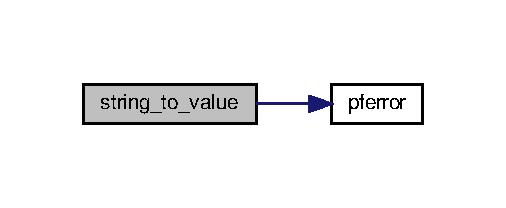
\includegraphics[width=243pt]{types_8h_a9c194ae881900b4376e761e2294117f9_cgraph}
\end{center}
\end{figure}
\mbox{\Hypertarget{types_8h_ab4456b47af2527b772ee8db5a367c66b}\label{types_8h_ab4456b47af2527b772ee8db5a367c66b}} 
\index{types.\+h@{types.\+h}!value\+\_\+new\+\_\+lint@{value\+\_\+new\+\_\+lint}}
\index{value\+\_\+new\+\_\+lint@{value\+\_\+new\+\_\+lint}!types.\+h@{types.\+h}}
\subsubsection{\texorpdfstring{value\+\_\+new\+\_\+lint()}{value\_new\_lint()}}
{\footnotesize\ttfamily \hyperlink{types_8h_ae4d4f561b975159d5852cb2c30bf20ef}{value\+\_\+t} value\+\_\+new\+\_\+lint (\begin{DoxyParamCaption}\item[{\hyperlink{types_8h_a5b2030ae244cd6621f11f4bf6d181dbf}{sys\+\_\+int\+\_\+long}}]{lint }\end{DoxyParamCaption})}

\mbox{\Hypertarget{types_8h_a82b79a7bbb2da51fd09d5f5c90c5105a}\label{types_8h_a82b79a7bbb2da51fd09d5f5c90c5105a}} 
\index{types.\+h@{types.\+h}!value\+\_\+new\+\_\+type@{value\+\_\+new\+\_\+type}}
\index{value\+\_\+new\+\_\+type@{value\+\_\+new\+\_\+type}!types.\+h@{types.\+h}}
\subsubsection{\texorpdfstring{value\+\_\+new\+\_\+type()}{value\_new\_type()}}
{\footnotesize\ttfamily \hyperlink{types_8h_ae4d4f561b975159d5852cb2c30bf20ef}{value\+\_\+t} value\+\_\+new\+\_\+type (\begin{DoxyParamCaption}\item[{enum \hyperlink{types_8h_a2763ddd86ab6e5f5f4c34c0561d4cd39}{value\+\_\+types}}]{type }\end{DoxyParamCaption})}

\mbox{\Hypertarget{types_8h_a4560a9f9bfc3ee07f105b16cc4230964}\label{types_8h_a4560a9f9bfc3ee07f105b16cc4230964}} 
\index{types.\+h@{types.\+h}!value\+\_\+to\+\_\+string@{value\+\_\+to\+\_\+string}}
\index{value\+\_\+to\+\_\+string@{value\+\_\+to\+\_\+string}!types.\+h@{types.\+h}}
\subsubsection{\texorpdfstring{value\+\_\+to\+\_\+string()}{value\_to\_string()}}
{\footnotesize\ttfamily void value\+\_\+to\+\_\+string (\begin{DoxyParamCaption}\item[{char $\ast$}]{dst\+\_\+str,  }\item[{\hyperlink{types_8h_ae4d4f561b975159d5852cb2c30bf20ef}{value\+\_\+t}}]{src\+\_\+val }\end{DoxyParamCaption})}

$<$ \begin{DoxyWarning}{Warning}
Unknown types of \hyperlink{types_8h_ae4d4f561b975159d5852cb2c30bf20ef}{value\+\_\+t} will just assert(false) here. 
\end{DoxyWarning}

\hypertarget{workspace_8c}{\section{workspace.\+c File Reference}
\label{workspace_8c}\index{workspace.\+c@{workspace.\+c}}
}
{\ttfamily \#include $<$string.\+h$>$}\\*
{\ttfamily \#include \char`\"{}errors.\+h\char`\"{}}\\*
{\ttfamily \#include \char`\"{}workspace.\+h\char`\"{}}\\*
Include dependency graph for workspace.\+c\+:\nopagebreak
\begin{figure}[H]
\begin{center}
\leavevmode
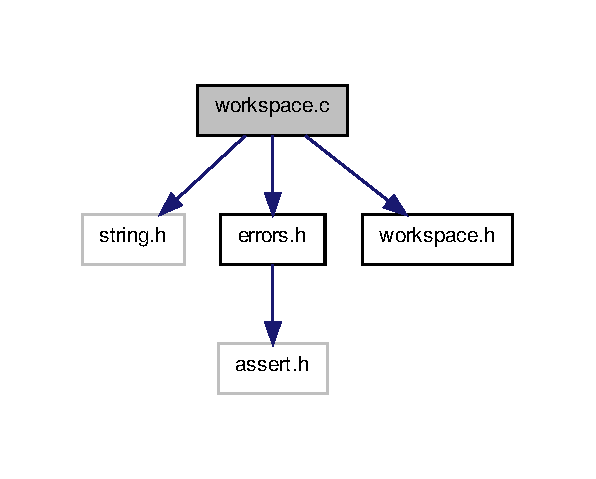
\includegraphics[width=286pt]{workspace_8c__incl}
\end{center}
\end{figure}
\subsection*{Data Structures}
\begin{DoxyCompactItemize}
\item 
struct {\bfseries workspace}
\end{DoxyCompactItemize}
\subsection*{Macros}
\begin{DoxyCompactItemize}
\item 
\#define \hyperlink{workspace_8c_aadf355de53cdc42e6a1081916321251f}{W\+S\+\_\+\+I\+S\+\_\+\+U\+N\+S\+E\+T}(x)~(W\+S\mbox{[}x\mbox{]}.name\mbox{[}0\mbox{]} == '\textbackslash{}0')
\item 
\#define \hyperlink{workspace_8c_a16aaa93198c62a638c59444212f025b8}{W\+S\+\_\+\+U\+N\+S\+E\+T}(x)~W\+S\mbox{[}x\mbox{]}.name\mbox{[}0\mbox{]} = '\textbackslash{}0'
\item 
\#define \hyperlink{workspace_8c_a2414aeb7dbcf5153e807c7f7d51e03b0}{W\+S\+\_\+\+L\+A\+S\+T}~ws\+\_\+last
\item 
\#define \hyperlink{workspace_8c_a0366a64834fcd82dd98ec57fbd4b1f46}{W\+S\+\_\+\+L\+A\+S\+T\+\_\+\+R\+E\+S\+E\+T}~ws\+\_\+last = -\/1
\item 
\#define \hyperlink{workspace_8c_a5bef065d3c4004e76f4226d41111c579}{W\+S\+\_\+\+L\+A\+S\+T\+\_\+\+S\+E\+T}(x)~ws\+\_\+last = ((x) $>$ ws\+\_\+last) ?(x)\+:ws\+\_\+last
\item 
\#define \hyperlink{workspace_8c_a273fa3245073307381a1ea8f71bf5151}{W\+S\+\_\+\+L\+A\+S\+T\+\_\+\+U\+N\+S\+E\+T}(x)~ws\+\_\+last = ((x) == ws\+\_\+last)?(ws\+\_\+last-\/1)\+:ws\+\_\+last
\item 
\#define \hyperlink{workspace_8c_aea36ffeb7e99fc5cbabe90b03f29cc02}{W\+S\+\_\+\+N\+O\+T\+F\+O\+U\+N\+D}~\hyperlink{workspace_8h_aab50c10161a2e913c9bd6c68a301d354}{W\+O\+R\+K\+S\+P\+A\+C\+E\+\_\+\+S\+I\+Z\+E}
\end{DoxyCompactItemize}
\subsection*{Functions}
\begin{DoxyCompactItemize}
\item 
void \hyperlink{workspace_8c_ae04d0019e903cb60b08ed382cb0b0d31}{workspace\+\_\+init} (void)
\begin{DoxyCompactList}\small\item\em Resets all workspace entries to unset. \end{DoxyCompactList}\item 
int \hyperlink{workspace_8c_a536b0f47bc3b9177d1aaca025a05515a}{workspace\+\_\+set} (char $\ast$name, void $\ast$data)
\item 
void \hyperlink{workspace_8c_a97b64b0cd36caba06d3c607cfb0c8dd8}{workspace\+\_\+unset} (char $\ast$name)
\item 
void $\ast$ \hyperlink{workspace_8c_a3af2e8d4387ce8986db09a9eb7328bc1}{workspace\+\_\+get} (char $\ast$name)
\end{DoxyCompactItemize}


\subsection{Detailed Description}
\begin{DoxyDate}{Date}
Apr 25, 2014 
\end{DoxyDate}
\begin{DoxyAuthor}{Author}
Craig Hesling 
\end{DoxyAuthor}


\subsection{Macro Definition Documentation}
\hypertarget{workspace_8c_aadf355de53cdc42e6a1081916321251f}{\index{workspace.\+c@{workspace.\+c}!W\+S\+\_\+\+I\+S\+\_\+\+U\+N\+S\+E\+T@{W\+S\+\_\+\+I\+S\+\_\+\+U\+N\+S\+E\+T}}
\index{W\+S\+\_\+\+I\+S\+\_\+\+U\+N\+S\+E\+T@{W\+S\+\_\+\+I\+S\+\_\+\+U\+N\+S\+E\+T}!workspace.\+c@{workspace.\+c}}
\subsubsection[{W\+S\+\_\+\+I\+S\+\_\+\+U\+N\+S\+E\+T}]{\setlength{\rightskip}{0pt plus 5cm}\#define W\+S\+\_\+\+I\+S\+\_\+\+U\+N\+S\+E\+T(
\begin{DoxyParamCaption}
\item[{}]{x}
\end{DoxyParamCaption}
)~(W\+S\mbox{[}x\mbox{]}.name\mbox{[}0\mbox{]} == '\textbackslash{}0')}}\label{workspace_8c_aadf355de53cdc42e6a1081916321251f}
\hypertarget{workspace_8c_a2414aeb7dbcf5153e807c7f7d51e03b0}{\index{workspace.\+c@{workspace.\+c}!W\+S\+\_\+\+L\+A\+S\+T@{W\+S\+\_\+\+L\+A\+S\+T}}
\index{W\+S\+\_\+\+L\+A\+S\+T@{W\+S\+\_\+\+L\+A\+S\+T}!workspace.\+c@{workspace.\+c}}
\subsubsection[{W\+S\+\_\+\+L\+A\+S\+T}]{\setlength{\rightskip}{0pt plus 5cm}\#define W\+S\+\_\+\+L\+A\+S\+T~ws\+\_\+last}}\label{workspace_8c_a2414aeb7dbcf5153e807c7f7d51e03b0}
\hypertarget{workspace_8c_a0366a64834fcd82dd98ec57fbd4b1f46}{\index{workspace.\+c@{workspace.\+c}!W\+S\+\_\+\+L\+A\+S\+T\+\_\+\+R\+E\+S\+E\+T@{W\+S\+\_\+\+L\+A\+S\+T\+\_\+\+R\+E\+S\+E\+T}}
\index{W\+S\+\_\+\+L\+A\+S\+T\+\_\+\+R\+E\+S\+E\+T@{W\+S\+\_\+\+L\+A\+S\+T\+\_\+\+R\+E\+S\+E\+T}!workspace.\+c@{workspace.\+c}}
\subsubsection[{W\+S\+\_\+\+L\+A\+S\+T\+\_\+\+R\+E\+S\+E\+T}]{\setlength{\rightskip}{0pt plus 5cm}\#define W\+S\+\_\+\+L\+A\+S\+T\+\_\+\+R\+E\+S\+E\+T~ws\+\_\+last = -\/1}}\label{workspace_8c_a0366a64834fcd82dd98ec57fbd4b1f46}
\hypertarget{workspace_8c_a5bef065d3c4004e76f4226d41111c579}{\index{workspace.\+c@{workspace.\+c}!W\+S\+\_\+\+L\+A\+S\+T\+\_\+\+S\+E\+T@{W\+S\+\_\+\+L\+A\+S\+T\+\_\+\+S\+E\+T}}
\index{W\+S\+\_\+\+L\+A\+S\+T\+\_\+\+S\+E\+T@{W\+S\+\_\+\+L\+A\+S\+T\+\_\+\+S\+E\+T}!workspace.\+c@{workspace.\+c}}
\subsubsection[{W\+S\+\_\+\+L\+A\+S\+T\+\_\+\+S\+E\+T}]{\setlength{\rightskip}{0pt plus 5cm}\#define W\+S\+\_\+\+L\+A\+S\+T\+\_\+\+S\+E\+T(
\begin{DoxyParamCaption}
\item[{}]{x}
\end{DoxyParamCaption}
)~ws\+\_\+last = ((x) $>$ ws\+\_\+last) ?(x)\+:ws\+\_\+last}}\label{workspace_8c_a5bef065d3c4004e76f4226d41111c579}
\hypertarget{workspace_8c_a273fa3245073307381a1ea8f71bf5151}{\index{workspace.\+c@{workspace.\+c}!W\+S\+\_\+\+L\+A\+S\+T\+\_\+\+U\+N\+S\+E\+T@{W\+S\+\_\+\+L\+A\+S\+T\+\_\+\+U\+N\+S\+E\+T}}
\index{W\+S\+\_\+\+L\+A\+S\+T\+\_\+\+U\+N\+S\+E\+T@{W\+S\+\_\+\+L\+A\+S\+T\+\_\+\+U\+N\+S\+E\+T}!workspace.\+c@{workspace.\+c}}
\subsubsection[{W\+S\+\_\+\+L\+A\+S\+T\+\_\+\+U\+N\+S\+E\+T}]{\setlength{\rightskip}{0pt plus 5cm}\#define W\+S\+\_\+\+L\+A\+S\+T\+\_\+\+U\+N\+S\+E\+T(
\begin{DoxyParamCaption}
\item[{}]{x}
\end{DoxyParamCaption}
)~ws\+\_\+last = ((x) == ws\+\_\+last)?(ws\+\_\+last-\/1)\+:ws\+\_\+last}}\label{workspace_8c_a273fa3245073307381a1ea8f71bf5151}
\hypertarget{workspace_8c_aea36ffeb7e99fc5cbabe90b03f29cc02}{\index{workspace.\+c@{workspace.\+c}!W\+S\+\_\+\+N\+O\+T\+F\+O\+U\+N\+D@{W\+S\+\_\+\+N\+O\+T\+F\+O\+U\+N\+D}}
\index{W\+S\+\_\+\+N\+O\+T\+F\+O\+U\+N\+D@{W\+S\+\_\+\+N\+O\+T\+F\+O\+U\+N\+D}!workspace.\+c@{workspace.\+c}}
\subsubsection[{W\+S\+\_\+\+N\+O\+T\+F\+O\+U\+N\+D}]{\setlength{\rightskip}{0pt plus 5cm}\#define W\+S\+\_\+\+N\+O\+T\+F\+O\+U\+N\+D~{\bf W\+O\+R\+K\+S\+P\+A\+C\+E\+\_\+\+S\+I\+Z\+E}}}\label{workspace_8c_aea36ffeb7e99fc5cbabe90b03f29cc02}
\hypertarget{workspace_8c_a16aaa93198c62a638c59444212f025b8}{\index{workspace.\+c@{workspace.\+c}!W\+S\+\_\+\+U\+N\+S\+E\+T@{W\+S\+\_\+\+U\+N\+S\+E\+T}}
\index{W\+S\+\_\+\+U\+N\+S\+E\+T@{W\+S\+\_\+\+U\+N\+S\+E\+T}!workspace.\+c@{workspace.\+c}}
\subsubsection[{W\+S\+\_\+\+U\+N\+S\+E\+T}]{\setlength{\rightskip}{0pt plus 5cm}\#define W\+S\+\_\+\+U\+N\+S\+E\+T(
\begin{DoxyParamCaption}
\item[{}]{x}
\end{DoxyParamCaption}
)~W\+S\mbox{[}x\mbox{]}.name\mbox{[}0\mbox{]} = '\textbackslash{}0'}}\label{workspace_8c_a16aaa93198c62a638c59444212f025b8}


\subsection{Function Documentation}
\hypertarget{workspace_8c_a3af2e8d4387ce8986db09a9eb7328bc1}{\index{workspace.\+c@{workspace.\+c}!workspace\+\_\+get@{workspace\+\_\+get}}
\index{workspace\+\_\+get@{workspace\+\_\+get}!workspace.\+c@{workspace.\+c}}
\subsubsection[{workspace\+\_\+get}]{\setlength{\rightskip}{0pt plus 5cm}void$\ast$ workspace\+\_\+get (
\begin{DoxyParamCaption}
\item[{char $\ast$}]{name}
\end{DoxyParamCaption}
)}}\label{workspace_8c_a3af2e8d4387ce8986db09a9eb7328bc1}
\begin{DoxyRefDesc}{Todo}
\item[\hyperlink{todo__todo000006}{Todo}]Create a return value for bad name like \hyperlink{workspace_8h_a536b0f47bc3b9177d1aaca025a05515a}{workspace\+\_\+set} with W\+O\+R\+K\+S\+P\+A\+C\+E\+\_\+\+N\+A\+M\+E \end{DoxyRefDesc}
\hypertarget{workspace_8c_ae04d0019e903cb60b08ed382cb0b0d31}{\index{workspace.\+c@{workspace.\+c}!workspace\+\_\+init@{workspace\+\_\+init}}
\index{workspace\+\_\+init@{workspace\+\_\+init}!workspace.\+c@{workspace.\+c}}
\subsubsection[{workspace\+\_\+init}]{\setlength{\rightskip}{0pt plus 5cm}void workspace\+\_\+init (
\begin{DoxyParamCaption}
\item[{void}]{}
\end{DoxyParamCaption}
)}}\label{workspace_8c_ae04d0019e903cb60b08ed382cb0b0d31}


Resets all workspace entries to unset. 

\begin{DoxyNote}{Note}
Must be run before workspace use. 
\end{DoxyNote}
\hypertarget{workspace_8c_a536b0f47bc3b9177d1aaca025a05515a}{\index{workspace.\+c@{workspace.\+c}!workspace\+\_\+set@{workspace\+\_\+set}}
\index{workspace\+\_\+set@{workspace\+\_\+set}!workspace.\+c@{workspace.\+c}}
\subsubsection[{workspace\+\_\+set}]{\setlength{\rightskip}{0pt plus 5cm}int workspace\+\_\+set (
\begin{DoxyParamCaption}
\item[{char $\ast$}]{name, }
\item[{void $\ast$}]{data}
\end{DoxyParamCaption}
)}}\label{workspace_8c_a536b0f47bc3b9177d1aaca025a05515a}
\hypertarget{workspace_8c_a97b64b0cd36caba06d3c607cfb0c8dd8}{\index{workspace.\+c@{workspace.\+c}!workspace\+\_\+unset@{workspace\+\_\+unset}}
\index{workspace\+\_\+unset@{workspace\+\_\+unset}!workspace.\+c@{workspace.\+c}}
\subsubsection[{workspace\+\_\+unset}]{\setlength{\rightskip}{0pt plus 5cm}void workspace\+\_\+unset (
\begin{DoxyParamCaption}
\item[{char $\ast$}]{name}
\end{DoxyParamCaption}
)}}\label{workspace_8c_a97b64b0cd36caba06d3c607cfb0c8dd8}

\hypertarget{workspace_8h}{}\section{workspace.\+h File Reference}
\label{workspace_8h}\index{workspace.\+h@{workspace.\+h}}
\subsection*{Macros}
\begin{DoxyCompactItemize}
\item 
\#define \hyperlink{workspace_8h_ad871f3f2b1ef4a985234d6d835df58dc}{W\+O\+R\+K\+S\+P\+A\+C\+E\+\_\+\+N\+A\+M\+E\+\_\+\+S\+I\+ZE}~10
\item 
\#define \hyperlink{workspace_8h_aab50c10161a2e913c9bd6c68a301d354}{W\+O\+R\+K\+S\+P\+A\+C\+E\+\_\+\+S\+I\+ZE}~10
\item 
\#define \hyperlink{workspace_8h_a8bd8e9e3cab867671a21a9e3315b59cd}{W\+O\+R\+K\+S\+P\+A\+C\+E\+\_\+\+N\+O\+T\+S\+ET}~((void $\ast$)(long)(-\/1))
\begin{DoxyCompactList}\small\item\em Indicates that a specified name has not been defined. For use in \hyperlink{workspace_8h_a3af2e8d4387ce8986db09a9eb7328bc1}{workspace\+\_\+get}. \end{DoxyCompactList}\item 
\#define \hyperlink{workspace_8h_a147135e1aa927764f2295f2c152476b0}{W\+O\+R\+K\+S\+P\+A\+C\+E\+\_\+\+OK}~0
\begin{DoxyCompactList}\small\item\em Indicates that the \hyperlink{workspace_8h_a536b0f47bc3b9177d1aaca025a05515a}{workspace\+\_\+set} operation was successful. \end{DoxyCompactList}\item 
\#define \hyperlink{workspace_8h_aef9978df27bbcf2ae8de42ec14ccb6fa}{W\+O\+R\+K\+S\+P\+A\+C\+E\+\_\+\+F\+U\+LL}~1
\begin{DoxyCompactList}\small\item\em Indicates that the \hyperlink{workspace_8h_a536b0f47bc3b9177d1aaca025a05515a}{workspace\+\_\+set} operation failed because the the workspace is full. \end{DoxyCompactList}\item 
\#define \hyperlink{workspace_8h_a1ae642ceb45b941c6c17cde25c57b3f1}{W\+O\+R\+K\+S\+P\+A\+C\+E\+\_\+\+N\+A\+ME}~2
\begin{DoxyCompactList}\small\item\em Indicates that the \hyperlink{workspace_8h_a536b0f47bc3b9177d1aaca025a05515a}{workspace\+\_\+set} operation failed because the the name argument is invalid. \end{DoxyCompactList}\end{DoxyCompactItemize}
\subsection*{Functions}
\begin{DoxyCompactItemize}
\item 
void \hyperlink{workspace_8h_ae04d0019e903cb60b08ed382cb0b0d31}{workspace\+\_\+init} (void)
\begin{DoxyCompactList}\small\item\em Resets all workspace entries to unset. \end{DoxyCompactList}\item 
int \hyperlink{workspace_8h_a536b0f47bc3b9177d1aaca025a05515a}{workspace\+\_\+set} (char $\ast$name, void $\ast$data)
\item 
void \hyperlink{workspace_8h_a97b64b0cd36caba06d3c607cfb0c8dd8}{workspace\+\_\+unset} (char $\ast$name)
\item 
void $\ast$ \hyperlink{workspace_8h_a3af2e8d4387ce8986db09a9eb7328bc1}{workspace\+\_\+get} (char $\ast$name)
\end{DoxyCompactItemize}


\subsection{Detailed Description}
\begin{DoxyDate}{Date}
Apr 25, 2014 
\end{DoxyDate}
\begin{DoxyAuthor}{Author}
Craig Hesling 
\end{DoxyAuthor}


\subsection{Macro Definition Documentation}
\mbox{\Hypertarget{workspace_8h_aef9978df27bbcf2ae8de42ec14ccb6fa}\label{workspace_8h_aef9978df27bbcf2ae8de42ec14ccb6fa}} 
\index{workspace.\+h@{workspace.\+h}!W\+O\+R\+K\+S\+P\+A\+C\+E\+\_\+\+F\+U\+LL@{W\+O\+R\+K\+S\+P\+A\+C\+E\+\_\+\+F\+U\+LL}}
\index{W\+O\+R\+K\+S\+P\+A\+C\+E\+\_\+\+F\+U\+LL@{W\+O\+R\+K\+S\+P\+A\+C\+E\+\_\+\+F\+U\+LL}!workspace.\+h@{workspace.\+h}}
\subsubsection{\texorpdfstring{W\+O\+R\+K\+S\+P\+A\+C\+E\+\_\+\+F\+U\+LL}{WORKSPACE\_FULL}}
{\footnotesize\ttfamily \#define W\+O\+R\+K\+S\+P\+A\+C\+E\+\_\+\+F\+U\+LL~1}



Indicates that the \hyperlink{workspace_8h_a536b0f47bc3b9177d1aaca025a05515a}{workspace\+\_\+set} operation failed because the the workspace is full. 

\mbox{\Hypertarget{workspace_8h_a1ae642ceb45b941c6c17cde25c57b3f1}\label{workspace_8h_a1ae642ceb45b941c6c17cde25c57b3f1}} 
\index{workspace.\+h@{workspace.\+h}!W\+O\+R\+K\+S\+P\+A\+C\+E\+\_\+\+N\+A\+ME@{W\+O\+R\+K\+S\+P\+A\+C\+E\+\_\+\+N\+A\+ME}}
\index{W\+O\+R\+K\+S\+P\+A\+C\+E\+\_\+\+N\+A\+ME@{W\+O\+R\+K\+S\+P\+A\+C\+E\+\_\+\+N\+A\+ME}!workspace.\+h@{workspace.\+h}}
\subsubsection{\texorpdfstring{W\+O\+R\+K\+S\+P\+A\+C\+E\+\_\+\+N\+A\+ME}{WORKSPACE\_NAME}}
{\footnotesize\ttfamily \#define W\+O\+R\+K\+S\+P\+A\+C\+E\+\_\+\+N\+A\+ME~2}



Indicates that the \hyperlink{workspace_8h_a536b0f47bc3b9177d1aaca025a05515a}{workspace\+\_\+set} operation failed because the the name argument is invalid. 

\mbox{\Hypertarget{workspace_8h_ad871f3f2b1ef4a985234d6d835df58dc}\label{workspace_8h_ad871f3f2b1ef4a985234d6d835df58dc}} 
\index{workspace.\+h@{workspace.\+h}!W\+O\+R\+K\+S\+P\+A\+C\+E\+\_\+\+N\+A\+M\+E\+\_\+\+S\+I\+ZE@{W\+O\+R\+K\+S\+P\+A\+C\+E\+\_\+\+N\+A\+M\+E\+\_\+\+S\+I\+ZE}}
\index{W\+O\+R\+K\+S\+P\+A\+C\+E\+\_\+\+N\+A\+M\+E\+\_\+\+S\+I\+ZE@{W\+O\+R\+K\+S\+P\+A\+C\+E\+\_\+\+N\+A\+M\+E\+\_\+\+S\+I\+ZE}!workspace.\+h@{workspace.\+h}}
\subsubsection{\texorpdfstring{W\+O\+R\+K\+S\+P\+A\+C\+E\+\_\+\+N\+A\+M\+E\+\_\+\+S\+I\+ZE}{WORKSPACE\_NAME\_SIZE}}
{\footnotesize\ttfamily \#define W\+O\+R\+K\+S\+P\+A\+C\+E\+\_\+\+N\+A\+M\+E\+\_\+\+S\+I\+ZE~10}

\mbox{\Hypertarget{workspace_8h_a8bd8e9e3cab867671a21a9e3315b59cd}\label{workspace_8h_a8bd8e9e3cab867671a21a9e3315b59cd}} 
\index{workspace.\+h@{workspace.\+h}!W\+O\+R\+K\+S\+P\+A\+C\+E\+\_\+\+N\+O\+T\+S\+ET@{W\+O\+R\+K\+S\+P\+A\+C\+E\+\_\+\+N\+O\+T\+S\+ET}}
\index{W\+O\+R\+K\+S\+P\+A\+C\+E\+\_\+\+N\+O\+T\+S\+ET@{W\+O\+R\+K\+S\+P\+A\+C\+E\+\_\+\+N\+O\+T\+S\+ET}!workspace.\+h@{workspace.\+h}}
\subsubsection{\texorpdfstring{W\+O\+R\+K\+S\+P\+A\+C\+E\+\_\+\+N\+O\+T\+S\+ET}{WORKSPACE\_NOTSET}}
{\footnotesize\ttfamily \#define W\+O\+R\+K\+S\+P\+A\+C\+E\+\_\+\+N\+O\+T\+S\+ET~((void $\ast$)(long)(-\/1))}



Indicates that a specified name has not been defined. For use in \hyperlink{workspace_8h_a3af2e8d4387ce8986db09a9eb7328bc1}{workspace\+\_\+get}. 

\mbox{\Hypertarget{workspace_8h_a147135e1aa927764f2295f2c152476b0}\label{workspace_8h_a147135e1aa927764f2295f2c152476b0}} 
\index{workspace.\+h@{workspace.\+h}!W\+O\+R\+K\+S\+P\+A\+C\+E\+\_\+\+OK@{W\+O\+R\+K\+S\+P\+A\+C\+E\+\_\+\+OK}}
\index{W\+O\+R\+K\+S\+P\+A\+C\+E\+\_\+\+OK@{W\+O\+R\+K\+S\+P\+A\+C\+E\+\_\+\+OK}!workspace.\+h@{workspace.\+h}}
\subsubsection{\texorpdfstring{W\+O\+R\+K\+S\+P\+A\+C\+E\+\_\+\+OK}{WORKSPACE\_OK}}
{\footnotesize\ttfamily \#define W\+O\+R\+K\+S\+P\+A\+C\+E\+\_\+\+OK~0}



Indicates that the \hyperlink{workspace_8h_a536b0f47bc3b9177d1aaca025a05515a}{workspace\+\_\+set} operation was successful. 

\mbox{\Hypertarget{workspace_8h_aab50c10161a2e913c9bd6c68a301d354}\label{workspace_8h_aab50c10161a2e913c9bd6c68a301d354}} 
\index{workspace.\+h@{workspace.\+h}!W\+O\+R\+K\+S\+P\+A\+C\+E\+\_\+\+S\+I\+ZE@{W\+O\+R\+K\+S\+P\+A\+C\+E\+\_\+\+S\+I\+ZE}}
\index{W\+O\+R\+K\+S\+P\+A\+C\+E\+\_\+\+S\+I\+ZE@{W\+O\+R\+K\+S\+P\+A\+C\+E\+\_\+\+S\+I\+ZE}!workspace.\+h@{workspace.\+h}}
\subsubsection{\texorpdfstring{W\+O\+R\+K\+S\+P\+A\+C\+E\+\_\+\+S\+I\+ZE}{WORKSPACE\_SIZE}}
{\footnotesize\ttfamily \#define W\+O\+R\+K\+S\+P\+A\+C\+E\+\_\+\+S\+I\+ZE~10}



\subsection{Function Documentation}
\mbox{\Hypertarget{workspace_8h_a3af2e8d4387ce8986db09a9eb7328bc1}\label{workspace_8h_a3af2e8d4387ce8986db09a9eb7328bc1}} 
\index{workspace.\+h@{workspace.\+h}!workspace\+\_\+get@{workspace\+\_\+get}}
\index{workspace\+\_\+get@{workspace\+\_\+get}!workspace.\+h@{workspace.\+h}}
\subsubsection{\texorpdfstring{workspace\+\_\+get()}{workspace\_get()}}
{\footnotesize\ttfamily void$\ast$ workspace\+\_\+get (\begin{DoxyParamCaption}\item[{char $\ast$}]{name }\end{DoxyParamCaption})}

\begin{DoxyRefDesc}{Todo}
\item[\hyperlink{todo__todo000006}{Todo}]Create a return value for bad name like \hyperlink{workspace_8h_a536b0f47bc3b9177d1aaca025a05515a}{workspace\+\_\+set} with W\+O\+R\+K\+S\+P\+A\+C\+E\+\_\+\+N\+A\+ME \end{DoxyRefDesc}
\mbox{\Hypertarget{workspace_8h_ae04d0019e903cb60b08ed382cb0b0d31}\label{workspace_8h_ae04d0019e903cb60b08ed382cb0b0d31}} 
\index{workspace.\+h@{workspace.\+h}!workspace\+\_\+init@{workspace\+\_\+init}}
\index{workspace\+\_\+init@{workspace\+\_\+init}!workspace.\+h@{workspace.\+h}}
\subsubsection{\texorpdfstring{workspace\+\_\+init()}{workspace\_init()}}
{\footnotesize\ttfamily void workspace\+\_\+init (\begin{DoxyParamCaption}\item[{void}]{ }\end{DoxyParamCaption})}



Resets all workspace entries to unset. 

\begin{DoxyNote}{Note}
Must be run before workspace use. 
\end{DoxyNote}
\mbox{\Hypertarget{workspace_8h_a536b0f47bc3b9177d1aaca025a05515a}\label{workspace_8h_a536b0f47bc3b9177d1aaca025a05515a}} 
\index{workspace.\+h@{workspace.\+h}!workspace\+\_\+set@{workspace\+\_\+set}}
\index{workspace\+\_\+set@{workspace\+\_\+set}!workspace.\+h@{workspace.\+h}}
\subsubsection{\texorpdfstring{workspace\+\_\+set()}{workspace\_set()}}
{\footnotesize\ttfamily int workspace\+\_\+set (\begin{DoxyParamCaption}\item[{char $\ast$}]{name,  }\item[{void $\ast$}]{data }\end{DoxyParamCaption})}

\mbox{\Hypertarget{workspace_8h_a97b64b0cd36caba06d3c607cfb0c8dd8}\label{workspace_8h_a97b64b0cd36caba06d3c607cfb0c8dd8}} 
\index{workspace.\+h@{workspace.\+h}!workspace\+\_\+unset@{workspace\+\_\+unset}}
\index{workspace\+\_\+unset@{workspace\+\_\+unset}!workspace.\+h@{workspace.\+h}}
\subsubsection{\texorpdfstring{workspace\+\_\+unset()}{workspace\_unset()}}
{\footnotesize\ttfamily void workspace\+\_\+unset (\begin{DoxyParamCaption}\item[{char $\ast$}]{name }\end{DoxyParamCaption})}


%--- End generated contents ---

% Index
\backmatter
\newpage
\phantomsection
\clearemptydoublepage
\addcontentsline{toc}{chapter}{Index}
\printindex

\end{document}
